\documentclass[german, 12pt, oneside, numbers=noenddot]{scrbook}
\usepackage{geometry}                		
%\usepackage{german}
%\usepackage{ngerman}
\usepackage[german]{babel}
%\usepackage[parfill]{parskip}    			% Activate to begin paragraphs with an empty line rather than an indent
\usepackage{graphicx}						% Use pdf, png, jpg, or epsß with pdflatex; use eps in DVI mode
											% TeX will automatically convert eps --> pdf in pdflatex		

%\usepackage{helvet}						% Kommentar wegnehmen, um in Helvetica zu schreiben
%\renewcommand{\familydefault}{\sfdefault}
%\fontfamily{phv}\selectfont

\usepackage{amssymb}
\usepackage{mathtools} % includes amsmath

\usepackage[utf8]{inputenc}
\usepackage[T1]{fontenc}

\usepackage{lscape}

%\usepackage{arydshln} attention: not compatible with longtable
\usepackage{tabularx}
\usepackage{longtable} % table over multiple pages
\usepackage{multirow}
\usepackage{subfig}
\usepackage{pdfpages}
\usepackage{framed}

\usepackage{forloop}								
\usepackage{listings}
\usepackage{fancyvrb}
\usepackage{color} 
\usepackage{colortbl}
\usepackage{courier}
\usepackage{pifont}

\usepackage[pdftex]{hyperref}
\usepackage{url}

\usepackage{float} % für \begin{figure}[H]
\usepackage{fancyhdr}
\usepackage{lipsum}

\usepackage{multicol} % für mehrspaltige Texte

\usepackage{scrhack}


%	%%%%%%%%%%%%%%%%%%%%%%%%%%%%%%%%%%%%%%%%%%%%%%%%%%%%%%%%
% 	Vermeiden der KOMA Script Fehlermeldung:
%      'Class scrbook Error: undefined old font command `\rm''	
%	%%%%%%%%%%%%%%%%%%%%%%%%%%%%%%%%%%%%%%%%%%%%%%%%%%%%%%%%

\makeatletter
\DeclareOldFontCommand{\rm}{\normalfont\rmfamily}{\mathrm}
\DeclareOldFontCommand{\sf}{\normalfont\sffamily}{\mathsf}
\DeclareOldFontCommand{\tt}{\normalfont\ttfamily}{\mathtt}
\DeclareOldFontCommand{\bf}{\normalfont\bfseries}{\mathbf}
\DeclareOldFontCommand{\it}{\normalfont\itshape}{\mathit}
\DeclareOldFontCommand{\sl}{\normalfont\slshape}{\@nomath\sl}
\DeclareOldFontCommand{\sc}{\normalfont\scshape}{\@nomath\sc}
\makeatother



%	%%%%%%%%%%%%%%%%%%%%%%%%%%%%%%%%%%%%%%%%%%%%%%%%%%%%%%%%
% 	Dokumentabmessungen	
%	%%%%%%%%%%%%%%%%%%%%%%%%%%%%%%%%%%%%%%%%%%%%%%%%%%%%%%%%

\geometry {a4paper, bottom=30mm, left=20mm, right=30mm, top=25mm}


%	%%%%%%%%%%%%%%%%%%%%%%%%%%%%%%%%%%%%%%%%%%%%%%%%%%%%%%%%
% 	Kopfzeile
%	%%%%%%%%%%%%%%%%%%%%%%%%%%%%%%%%%%%%%%%%%%%%%%%%%%%%%%%%

\pagestyle{fancyplain}
\fancyhf{}

% Kopfzeile links: Kapitel rechts: HTL Logo
\lhead{\fancyplain{}{\nouppercase\leftmark}}
\rhead{\fancyplain{}{
\includegraphics[width=2cm]{./media/images/htl_moedling_logo.jpg}}}

%\cfoot{\fancyplain{\thepage}{}}
%\rfoot{\fancyplain{}{\thepage}} %-----------------------


% Auskommentieren der folgenden Zeile setzt das HTL Logo in die
% Mitte der Kopfzeile auf jeder ersten Haupt-Kapitelseite

%\chead{\fancyplain{
\includegraphics[width=1.5cm]{./media/images/htl_moedling_logo.jpg}}{}}


%	%%%%%%%%%%%%%%%%%%%%%%%%%%%%%%%%%%%%%%%%%%%%%%%%%%%%%%%%
% 	Farbdefinitionen	
%	%%%%%%%%%%%%%%%%%%%%%%%%%%%%%%%%%%%%%%%%%%%%%%%%%%%%%%%%

\definecolor{grey}{RGB}{127,127,127}
\definecolor{lightgrey}{RGB}{180,180,180}
\definecolor{dkgreen}{rgb}{0,0.6,0}  
\definecolor{gray}{rgb}{0.5,0.5,0.5} 
\definecolor{mauve}{rgb}{0.58,0,0.82}

\definecolor{cssId}{rgb}		{0,0,0.6 }%{0.75, 0.00, 0.00 }
\definecolor{cssAttribute}{rgb}	{0.58,0,0.82 }%{0.00, 0.00, 0.75 }
\definecolor{cssClass}{rgb}		{0,0,0.6 }%{0.00, 0.75, 0.00 }
\definecolor{cssComment}{rgb}	{0,0.6,0 }%{0.00, 0.75, 0.00 }
\definecolor{cssString}{rgb}	{0.6,0,0 }%{0.00, 0.75, 0.00 }



%	%%%%%%%%%%%%%%%%%%%%%%%%%%%%%%%%%%%%%%%%%%%%%%%%%%%%%%%%
% 	Diverse Befehle		
%	%%%%%%%%%%%%%%%%%%%%%%%%%%%%%%%%%%%%%%%%%%%%%%%%%%%%%%%%

%	Quelltext im Textfluss
\def\inlinecode#1{\texttt{\color{gray}{#1}}}


%	Paragraph mit Zeilenumbruch nachher
\def\htlParagraph#1{\paragraph*{#1}$\;$ \\}

%   Short Version of \today
\newcommand{\leadingzero}[1]{\ifnum #1<10 0\the#1\else\the#1\fi}
\newcommand{\todayshort}{\leadingzero{\day}.\leadingzero{\month}.\the\year}

%	%%%%%%%%%%%%%%%%%%%%%%%%%%%%%%%%%%%%%%%%%%%%%%%%%%%%%%%%
% 	Code Formatierung		
%	%%%%%%%%%%%%%%%%%%%%%%%%%%%%%%%%%%%%%%%%%%%%%%%%%%%%%%%%
\lstset{literate=%
{Ö}{{\"O}}1 
{Ä}{{\"A}}1 
{Ü}{{\"U}}1 
{ß}{{\ss}}2 
{ü}{{\"u}}1 
{ä}{{\"a}}1 
{ö}{{\"o}}1
}
 
\lstset{ % 
%  language=Octave,                			% the language of the code 
 	basicstyle=\ttfamily\footnotesize, 		% the size of the fonts that are used for the code 
	numbers=left,                   		% where to put the line-numbers 
	numberstyle=\tiny\color{gray},  		% the style that is used for the line-numbers 
	stepnumber=1,                   		% the step between two line-numbers. If it's 1, each line  
                                  			% will be numbered 
	numbersep=5pt,                  		% how far the line-numbers are from the code 
	backgroundcolor=\color{white},    	  	% choose the background color. You must add \usepackage{color}
	showspaces=false,               		% show spaces adding particular underscores 
	showstringspaces=false,      	   		% underline spaces within strings
	showtabs=false,                 		% show tabs within strings adding particular underscores
%	frame=single,                   		% adds a frame around the code
	frame=l,
	rulecolor=\color{dkgreen},        		% if not set, the frame-color may be changed on line-breaks within not-black text (e.g. comments (green here))
	tabsize=2,                      		% sets default tabsize to 2 spaces
	captionpos=b,                   		% sets the caption-position to bottom
	breaklines=true,                		% sets automatic line breaking
	breakatwhitespace=false,        		% sets if automatic breaks should only happen at whitespace
%	title=\lstname,                   		% show the filename of files included with \lstinputlisting;
          	                        		% also try caption instead of title
	keywordstyle=\color{blue},          	% keyword style
	commentstyle=\color{dkgreen},       	% comment style
	stringstyle=\color{mauve},    	     	% string literal style
	escapeinside={\%*}{*)},            		% if you want to add LaTeX within your code
	morekeywords={*,...},              		% if you want to add more keywords to the set
	deletekeywords={...}             	 	% if you want to delete keywords from the given language
}

%	%%%%%%%%%%%%%%%%%%%%%%%%%%%%%%%%%%%%%%%%%%%%%%%%%%%%%%%%
% 	CSS		
\lstdefinelanguage{CSS}{
		alsoletter={\\,/,*,:,-,\#,.},
		identifierstyle=\idstyle,
        keywords={accelerator:, azimuth:, background:, background-attachment:, background-color:, background-image:, background-position:, background-position-x:, background-position-y:, background-repeat:, behavior:, border:, border-bottom:, border-bottom-color:, border-bottom-style:, border-bottom-width:, border-collapse:, border-color:, border-left:, border-left-color:, border-left-style:, border-left-width:, border-right:, border-right-color:, border-right-style:, border-right-width:, border-spacing:, border-style:, border-top:, border-top-color:, border-top-style:, border-top-width:, border-width:, bottom   :, caption-side:, clear:, clip:, color:, content:, counter-increment:, counter-reset:, cue:, cue-after:, cue-before:, cursor:, direction:, display:, elevation:, empty-cells :, filter:, float:, font:, font-family:, font-size:, font-size-adjust:, font-stretch:, font-style:, font-variant:, font-weight:, height:, ime-mode:, include-source:, layer-background-color:, layer-background-image:, layout-flow:, layout-grid:, layout-grid-char:, layout-grid-char-spacing:, layout-grid-line:, layout-grid-mode:, layout-grid-type:, left:, letter-spacing:, line-break:, line-height:, list-style:, list-style-image:, list-style-position:, list-style-type:, margin:, margin-bottom:, margin-left:, margin-right:, margin-top:, marker-offset:, marks:, max-height:, max-width:, min-height:, min-width:, -moz-binding:, -moz-border-radius:, -moz-border-radius-topleft:, -moz-border-radius-topright:, -moz-border-radius-bottomright:, -moz-border-radius-bottomleft:, -moz-border-top-colors:, -moz-border-right-colors:, -moz-border-bottom-colors:, -moz-border-left-colors:, -moz-opacity:, -moz-outline:, -moz-outline-color:, -moz-outline-style:, -moz-outline-width:, -moz-user-focus:, -moz-user-input:, -moz-user-modify:, -moz-user-select:, orphans:, outline:, outline-color:, outline-style:, outline-width:, overflow:, overflow-X:, overflow-Y:, padding:, padding-bottom:, padding-left:, padding-right:, padding-top:, page:, page-break-after:, page-break-before:, page-break-inside:, pause:, pause-after:, pause-before:, pitch:, pitch-range:, play-during:, position:, quotes:, -replace:, richness:, right:, ruby-align:, ruby-overhang:, ruby-position:, -set-link-source:, size:, speak:, speak-header:, speak-numeral:, speak-punctuation:, speech-rate:, stress:, scrollbar-arrow-color:, scrollbar-base-color:, scrollbar-dark-shadow-color:, scrollbar-face-color:, scrollbar-highlight-color:, scrollbar-shadow-color:, scrollbar-3d-light-color:, scrollbar-track-color :, table-layout:, text-align:, text-align-last:, text-decoration:, text-indent:, text-justify:, text-overflow:, text-shadow:, text-transform:, text-autospace:, text-kashida-space:, text-underline-position:, top:, unicode-bidi:, -use-link-source:, vertical-align:, visibility:, voice-family:, volume :, white-space:, widows:, width:, word-break:, word-spacing:, word-wrap:, writing-mode},
        keywordstyle=\color{cssAttribute},%\bfseries,
        ndkeywords={@import, @media, @page, @font-face, @charset, @namespace, a, html, body, title, pre, h1, h2, h3, h4, h5, h6, ul, ol, li, p, br, blockquote, dl, dt, dd, div, img, strong, em, cite, tt, i, b, table, tr, td, th, frame, form, option, input, button, nav, section, article, aside, footer, hr, sup, sub, del, ins, small, span},
        ndkeywordstyle=\color{cssId},%,\bfseries,
%        identifierstyle=\color{black},
%        sensitive=false,
%        comment=[l]{//},
        morecomment=[s]{/*}{*/},
        commentstyle=\color{cssComment}\ttfamily,
        stringstyle=\color{cssString}\ttfamily,
        morestring=[b]',
        morestring=[b]"
}

\makeatletter
\newcommand*\idstyle[1]{%
         \expandafter\id@style\the\lst@token{#1}\relax%
 }

 \def\id@style#1#2\relax{%
           	\ifnum\pdfstrcmp{#1}{\#}=0%
                \small\ttfamily\color{cssId} \the\lst@token%
            \else%
		      	\ifnum\pdfstrcmp{#1}{.}=0%
    	            \small\ttfamily\color{cssClass} \the\lst@token%
        		\else%
					\ifnum\pdfstrcmp{#1}{:}=0%
    	            	\small\ttfamily\color{cssAttribute} \the\lst@token%
    	         	\else%
		     	 		%\edef\tempa{\uccode#1}%
              			\edef\tempa{\lccode`#1}%
              			\edef\tempb{`#1}%
              			\ifnum\tempa=\tempb%
                			\small\ttfamily\color{mauve} \the\lst@token%
              			\else%
                 	 		\the\lst@token%
    	         		\fi%
	           		\fi%
	            \fi%
            \fi%
 }
\makeatother



%	%%%%%%%%%%%%%%%%%%%%%%%%%%%%%%%%%%%%%%%%%%%%%%%%%%%%%%%%
% 	JavaScript	
\lstdefinelanguage{JavaScript}{
        keywords={typeof, new, true, false, catch, function, return, null, catch, switch, var, if, in, while, do, else, case, break},
		alsoletter={\{,\}\\,/,*,:,-,\#,.},
 %       keywordstyle=\color{blue}\bfseries,
        ndkeywords={class, export, boolean, throw, implements, import, this},
%        ndkeywordstyle=\color{darkgray}\bfseries,
%        identifierstyle=\color{black},
%        sensitive=false,
        comment=[l]{//},
        morecomment=[s]{/*}{*/},
%        commentstyle=\color{purple}\ttfamily,
%        stringstyle=\color{red}\ttfamily,
        morestring=[b]',
        morestring=[b]"
}



%	%%%%%%%%%%%%%%%%%%%%%%%%%%%%%%%%%%%%%%%%%%%%%%%%%%%%%%%%
% 	TypoScript	
\lstdefinelanguage{TypoScript}{
        keywords={typeof, new, true, false, catch, function, return, null, catch, switch, var, if, in, while, do, else, case, break},
		alsoletter={\{,\}\\,/,*,:,-,\#,.},
 %       keywordstyle=\color{blue}\bfseries,
        ndkeywords={class, export, boolean, throw, implements, import, this},
%        ndkeywordstyle=\color{darkgray}\bfseries,
%        identifierstyle=\color{black},
%        sensitive=false,
        comment=[l]{//},
        morecomment=[s]{/*}{*/},
%        commentstyle=\color{purple}\ttfamily,
%        stringstyle=\color{red}\ttfamily,
        morestring=[b]',
        morestring=[b]"
}
	

\usepackage[onehalfspacing]{setspace}
\usepackage{csquotes}
\usepackage{graphicx}
\usepackage{uarial} % Load uarial package for Arial font

% C#
\usepackage{listings}

% Fußnotenpackage
\usepackage{fancyhdr}
\usepackage{lastpage}

% to_donotes
\usepackage{todonotes}

% highlighting
\usepackage{xcolor, soul}

% german
%\usepackage[ngerman]{babel}

% ende
\newcommand{\newglossaryentryfast}[3]{%
    \newglossaryentry{#1}{%
        name={#2},
        description={#3},
    }
}

\lstdefinelanguage{CSharp}
{
    language=[Sharp]C,
    keywordstyle=\color{blue},
    commentstyle=\color{green!50!black},
    stringstyle=\color{red},
    morekeywords={var,get,set}
}

% Definieren eines neuen Befehls für die Fußzeile mit einem Parameter für den Namen
%\newcommand{\myfooter}[1]{
% \fancyfoot[C]{HTBLuVA-Mödling \hfill #1 \hfill Seite \thepage\ von \pageref{LastPage}}
%}

% Define a new page style 'customfooter' with the footer
\fancypagestyle{customfooter}{
  \fancyfoot[C]{HTBLuVA-Mödling \hfill \authorname \hfill Seite \thepage\ von \pageref{LastPage}}
}

% Command to set the author name for the footer
\newcommand{\setauthorname}[1]{\def\authorname{#1}}

% Default page style without the footer
\pagestyle{empty}

\newcommand{\bettergls}[2]{%
  \gls{#1}\footnote[#2]{\glsentrydesc{#1}}%
}


\usepackage[sort=use]{glossaries}
\makenoidxglossaries
\newglossaryentryfast{multiplayer}{Multiplayer}{Beschreibt den Videospiel Modus bei dem mehrere Menschen mit oder gegeneinander spielen}

\newglossaryentryfast{UI}{User Interface}{Beschreibt die Schnittstelle zwischen Mensch und Computer}

\newglossaryentryfast{singleplayer}{Singleplayer}{Beschreibt...}

\newglossaryentryfast{theme}{Theme}{Beschreibt...}

\newglossaryentryfast{canvas}{Canvas}{Beschreibung...}

\newglossaryentryfast{gameObject}{Game-Objekt}{Beschreibung...}

\newglossaryentryfast{skybox}{Skybox}{Beschreibt}

\newglossaryentryfast{code-behind}{Code-behind}{Ist...}

\newglossaryentryfast{statemachine}{State Machine}{...}

\newglossaryentryfast{jumprun}{Jump'n'Run}{Ist ...}

\newglossaryentryfast{boxcollider}{Box-Collider}{Ist...}
%\glsaddallunused % if glossar is acting up

\usepackage[ natbib=true, style=numeric,sorting=none]{biblatex}
\addbibresource{media/literatur.bib}

% Initialen der Autoren
\def\authorInitialsA{LS} % Lukas Schachinger
\def\authorInitialsB{UM} % Usta Martin

% Die Initialen werden verwendet um anzuzeigen wer welches Kapitel
% erstellt hat.h

% Die Befehle \authorA - \authorB werden in den Kapitelüberschriften angefügt
\def\authorA{\textmd{\textsuperscript{\authorInitialsA}}}
\def\authorB{\textmd{\textsuperscript{\authorInitialsB}}}

% Titel der Arbeit:
\def\htlArbeitsthema{Unity Game Design und Development}	

%\setlength{\headheight}{23.5071pt}
\setlength{\headheight}{23.7771pt}
\addtolength{\topmargin}{-6.5071pt}

% noindent
\setlength\parindent{0pt}

\begin{document}
\setauthorname{}
\pagestyle{customfooter}


\pagenumbering{arabic}	
		
% !TEX root = ../Vorlage_DA.tex

%	########################################################
% 							Deckblatt
%	########################################################


\titlehead{%
\begin{tabular}{@{}lcr@{}}
\raisebox{-0.5\height}{
\includegraphics[width=0.15\linewidth]{media/images/htl_moedling.png}} &
\begin{minipage}[c]{0.7\linewidth}
\begin{center}
{\bfseries\sffamily\large HÖHERE TECHNISCHE BUNDES - LEHR- UND\\[0.2em]
VERSUCHSANSTALT MÖDLING}\\[1ex]
{\normalsize Höhere Lehranstalt für Elektronik und Technische Informatik\\
Kolleg für Informatik}
{\textcolor{gray}{bzw. Aufbaulehrgang für Informatik}}
\end{center}
\end{minipage} &
\raisebox{-0.5\height}{
\includegraphics[width=0.15\linewidth]{media/images/htl-bildung-mit-zukunft}}
\end{tabular} \\ \\
\rule{1.05\linewidth}{0.4pt}
}

\title{\htlArbeitsthema}
\subtitle{ {\Large Diplomarbeit}\\[1em]Schulautonomer Schwerpunkt\\ Programmieren und Software Engineering}

\author{\\[1em] 
\emph{ausgeführt im Schuljahr 2022/2023 von:} \\[1em] 
Lukas Schachinger, 6AAIFT\\[1ex] 
Martin Usta, 6AAIFT\\[2em]
\emph{Betreuer:} \\[1em]
 Dipl.-Ing. Niklas Hack
}
\date{\today}

\begin{titlepage}	
\maketitle
\end{titlepage}

\chapter*{Eidesstattliche Erklärung}
\addcontentsline{toc}{chapter}{Eidesstattliche Erklärung}

Ich/Wir erkläre/n an Eides statt, dass ich/wir die vorliegende Diplomarbeit selbstständig und ohne fremde Hilfe verfasst, andere als angegebene Quellen und Hilfsmittel nicht direkt benutzt und die benutzten Quellen wörtlich und inhaltlich entnommenen Stellen als solche erkenntlich gemacht habe/n.
\vspace{3cm}

\begin{tabularx}{\textwidth}{l p{1cm} l p{1cm} X}


Mödling, \todayshort & & Lukas Schachinger & & \hrulefill \\
\emph{Ort, Datum} & & \emph{Verfasser} & & \emph{Unterschrift} \vspace{2cm}\\ 

Mödling, \todayshort & & Martin Usta & & \hrulefill \\
\emph{Ort, Datum} & & \emph{Verfasser} & & \emph{Unterschrift} \vspace{2cm}\\ 

\end{tabularx}

\chapter*{Dokumentation}
\addcontentsline{toc}{chapter}{Dokumentation}

\renewcommand{\arraystretch}{2} % Anpassen der Zeilenhöhe

\begin{tabular}{|m{0.3\textwidth}|m{0.7\textwidth}|}
\hline
Namen der Verfasser/innen & Lukas Schachinger, Martin Usta \\
\hline
Jahrgang & 5AAIFT / 6AAIFT \\
\hline
Thema der Diplomarbeit & Das Thema der Diplomarbeit ist Unity Game Design und Development. Es wird mithilfe der Dokumentation und eines spielbaren Prototyps gezeigt, wie man ein Spiel entwickelt. 
In der Dokumentation werden die Vorgehensweisen und die Programme, welche verwendetet werden beschrieben. \\
\hline
Kooperationspartner & / \\
\hline
\end{tabular}

\vspace{10pt}

\noindent
\begin{tabular}{|m{0.3\textwidth}|m{0.7\textwidth}|}
\hline
Aufgabenstellung & Teilaufgabe von Lukas Schachinger: \newline \newline Programmierung der physikalischen Grundfunktionen und Implementierung und Design einer grafischen Benutzeroberfläche \newline \newline Teilaufgabe von Martin Usta: \newline \newline Aufbau der 3D Spielewelt und Design der verschiedenen Level. Programmierung und Design der aktiven Spielfiguren. Implementierung der Musik und Soundeffekte der Spielumgebung.\\
\hline
\end{tabular}

\pagebreak

\noindent
\begin{tabular}{|m{0.3\textwidth}|m{0.7\textwidth}|}
\hline
Realisierung & Die Spielobjekte werden mithilfe von Blender designet und modelliert. \newline \newline Der Prototyp wird in Unity realisiert. Die fertigen Assets werden in Unity integriert und dann in das Spiel eingebaut. \newline \newline In C\# werden die Skripte geschrieben und dann an die Spielobjekte gebunden. \\
\hline
\end{tabular}

\vspace{10pt}

\noindent
\begin{tabular}{|m{0.3\textwidth}|m{0.7\textwidth}|}
\hline
Ergebnisse & Das Ergebnis wird ein spielbarer Prototyp sowie eine umfassende Dokumentation zum Thema Spieleentwicklung. Es soll mithilfe der Dokumentation erkennbar sein wie der Prototyp geplant und entwickelt wurde.  \\
\hline
\end{tabular}

\pagebreak

\noindent
\begin{tabular}{|m{0.3\textwidth}|m{0.7\textwidth}|}
\hline
Typische Grafik, Foto etc. (mit Erläuterung) & \\
\hline
\end{tabular}

\vspace{10pt}

\noindent
\begin{tabular}{|m{0.3\textwidth}|m{0.7\textwidth}|}
\hline
Teilnahme an Wettbewerben, Auszeichnungen & Keine \\
\hline
\end{tabular}

\vspace{10pt}

\noindent
\begin{tabular}{|m{0.3\textwidth}|m{0.7\textwidth}|}
\hline
Möglichkeiten der Einsichtnahme in die Arbeit & Im Archiv der Abteilung Elektronik und Technische Informatik der HTL Mödling \\
\hline
\end{tabular}

\vspace{10pt}

\noindent
\begin{tabular}{|m{0.325\textwidth}|m{0.325\textwidth}|m{0.325\textwidth}|}
\hline
Approbation (Datum / Unterschrift) & {\tiny Prüfer/Prüferin} \newline \newline & {\tiny Direktor/Direktorin} \newline {\tiny Abteilungsvorstand/Abteilungsvorständin} \newline \newline \\
\hline
\end{tabular}

\pagebreak

%here english ----------------------------------------------------------------

\noindent
\begin{tabular}{|m{0.3\textwidth}|m{0.7\textwidth}|}
\hline
Authors & Lukas Schachinger, Martin Usta \\
\hline
Academic Year & 5AAIFT / 6AAIFT \\
\hline
Topic & The topic of the diploma thesis is Unity Game Design and Development. It demonstrates the process of developing a game through documentation and a playable prototype. The documentation describes the methodologies and programs used. \\
\hline
Collaboration Partners & / \\
\hline
\end{tabular}

\vspace{10pt}

\noindent
\begin{tabular}{|m{0.3\textwidth}|m{0.7\textwidth}|}
\hline
Assignment & Subtask by Lukas Schachinger: \newline \newline Programming of the physics functions and implementation and design of a graphical user interface \newline \newline Subtask by Martin Usta: \newline \newline Construction of the 3D game world and design of various levels. Programming and design of active game characters. Implementation of music and sound effects in the game environment.\\
\hline
\end{tabular}

\pagebreak

\noindent
\begin{tabular}{|m{0.3\textwidth}|m{0.7\textwidth}|}
\hline
Implementation & The game objects are designed and modeled using Blender. \newline \newline The prototype is implemented in Unity. The finished assets are integrated into Unity and then incorporated into the game. \newline \newline The scripts are written in C\# and then bound to the game objects. \\
\hline
\end{tabular}

\vspace{10pt}

\noindent
\begin{tabular}{|m{0.3\textwidth}|m{0.7\textwidth}|}
\hline
Results & The result is a playable prototype and a detailed documentation on game development. The documentation should demonstrate how the prototype was planned and developed.  \\
\hline
\end{tabular}

\pagebreak

\noindent
\begin{tabular}{|m{0.3\textwidth}|m{0.7\textwidth}|}
\hline
Typical Graphics, Photos, etc. (with explanation) & \\
\hline
\end{tabular}

\vspace{10pt}

\noindent
\begin{tabular}{|m{0.3\textwidth}|m{0.7\textwidth}|}
\hline
Participation in Competitions, Awards & None \\
\hline
\end{tabular}

\vspace{10pt}

\noindent
\begin{tabular}{|m{0.3\textwidth}|m{0.7\textwidth}|}
\hline
Accessibility of \newline Diploma Thesis & Stored in the archive of the secondary technical college of Moedling, department of electronics and computer engineering \\
\hline
\end{tabular}

\vspace{10pt}

\noindent
\begin{tabular}{|m{0.325\textwidth}|m{0.325\textwidth}|m{0.325\textwidth}|}
\hline
Approval (Date / Signature) & {\tiny Examiner \newline \newline} & {\tiny Head of College / Department \newline \newline} \\
\hline
\end{tabular}

	
\tableofcontents

\pagebreak
\setauthorname{Lukas Schachinger \& Martin Usta}
\chapter{Pflichtenheft}
\section{Zielbestimmung}
\subsection{Musskriterien}

Es soll eine spielbare Demo erstellt werden. Dabei wird dem Spieler ein Charakter zur Verfügung gestellt, mit dem er sich in einer Spielwelt bewegen kann. Diese Spielwelt besteht aus verschiedenen selbst entworfenen Leveln. Es soll eine benutzerfreundliche Benutzeroberfläche geben, die aktuelle Spielinformationen anzeigt.

Zusätzlich wird eine Dokumentation erstellt, in der beschrieben wird, wie der Prototyp entwickelt wurde und welche Programme dabei verwendet wurden.

Musskriterien:
\begin{itemize}
  \item Spiele-Demo
  \begin{itemize}
    \item Spieler-Charakter
    \item Spielewelt
    \item Level-Design
  \end{itemize}
  \item Evaluierung von Programmen zur Spieleentwicklung
  \begin{itemize}
    \item Design: Blender, Material Design (selbstgestaltet/Download aus dem Internet)
    \item Game Engine: Unity
    \item Musik: (Musik-Software)
  \end{itemize}
\end{itemize}

\subsection{Wunschkriterien}
(TODO: 
Detaillierte Beschreibung der optionalen DA-Teile.)

\begin{itemize}
  \item Multiplayer
  \item Verbesserte künstliche Intelligenz (AI)
\end{itemize}

\subsection{Abgrenzungskriterien}
(TODO: 
Was ist nicht Teil der Arbeit.) %todo: mehr...

\begin{itemize}
  \item Kein vollständiges Spiel
  \item Kein VR-Spiel
\end{itemize}

\section{Projektumfeldanalyse}
Diese Arbeit baut nicht auf bestehenden Projekten auf.

\chapter{Projektplan}
\section{Gesamtprojektplan}

\newcolumntype{C}[1]{>{\centering\arraybackslash}p{#1}}

\noindent
\begin{tabular}{|C{3cm}|C{3cm}|C{3cm}|C{3cm}|C{3cm}|}
\hline
\multicolumn{5}{|c|}{\cellcolor{green!20} Projekt} \\
\hline
\cellcolor{green!20}Analyse des Umfelds/Projektplanung & & & & \\
\hline
& \cellcolor{green!20} Erstellung des Grundgerüsts für den Prototyp & & & \\
\hline
& & \cellcolor{green!20} Fertigstellung der UI & & \\
\hline
& & & \cellcolor{green!20} Fertigstellung des Prototyps & \\
\hline
& & & & \cellcolor{green!20} Diplomarbeit Fertigstellen \\
\hline
\end{tabular}


\vspace{10pt}

\noindent
\begin{tabular}{|C{2.43cm}|C{2.43cm}|C{2.43cm}|C{2.43cm}|C{2.43cm}|C{2.43cm}|C{2.43cm}|}
    Projektstart & Meilenstein 1 Ende & Meilenstein 2 Ende & Meilenstein 3 Ende & Meilenstein 4 Ende & Meilenstein 5 Ende \\
    01.09.2022 & 30.11.2022 & 18.12.2022 & 28.02.2023 & 31.05.2023 & 01.09.2023 \\
\end{tabular}


\pagebreak

\section{Meilensteine}
\subsection{Analyse des Umfelds / Projektplanung}
Zeitraum: 01.09.2022 – 30.11.2022\\\\
Tätigkeiten:
\begin{itemize}
    \item Recherche der Programme
    \item Recherche der Spiel-Engines
    \item Umfeldanalyse Unity gegen Unreal Engine
    \item Umfeldanalyse der unterschiedlichen Modellierprogramme
    \item Kategorisierung der Projektschwerpunkte
    \item Zeiteinteilung der Projektschwerpunkte
    \item Einrichtung des Projektmanagementtools 
\end{itemize}

\subsection{Erstellung des Grundgerüsts für den Prototyps}
Zeitraum: 30.11.2022 – 18.12.2022\\\\
Tätigkeiten:
\begin{itemize}
    \item Erstellung der Low-Poly Assets
    \item Design und Aufbau des ersten Levels 
    \item Implementierung der Charaktersteuerung
    \item Implementierung der beweglichen Plattformen
    \item Design und Integration der ersten Spielfiguren
\end{itemize}
\pagebreak

\subsection{Fertigstellung des UI}
Zeitraum 18.12.2022 – 28.02.2023\\\\
Tätigkeiten:
\begin{itemize}
    \item Planung des UI für eine optimale User Experience
    \item Aufbau und Erstellung einer Menuführung
    \item Erstellung einer Statistikoberfläche
\end{itemize}

\subsection{Fertigstellen des Prototyps}
Zeitraum 28.02.2023 – 31.05.2023\\\\
Tätigkeiten:
\begin{itemize}
    \item Bugs fixen
    \item Implementierung der High-Poly Assets
    \item Fertigstellung der Designaufgaben
    \item Fertigstellung der Programmieraufgaben
\end{itemize}

\subsection{Diplomarbeit fertigstellen}
Zeitraum 31.05.2023 – 01.09.2023\\\\
Tätigkeiten:
\begin{itemize}
    \item Fertigstellung der Dokumentation
\end{itemize}


\pagebreak

\section{Analyse des Umfelds / Projektplanung}
\begin{tabular}{|m{0.7\textwidth}|m{0.3\textwidth}|}
\hline
\multicolumn{2}{|c|}{\textbf{Analyse des Umfelds / Projektplanung von 01.09.2022 bis 30.11.2022}} \\
\hline
Tätigkeit & Hauptverantwortliche/r \\
\hline
Recherche der Programme & Schachinger, Usta \\
\hline
Recherche der Spiel-Engines & Schachinger \\
\hline
Umfeldanalyse Unity gegen Unreal Engine & Schachinger \\
\hline
Umfeldanalyse der unterschiedlichen Modellierprogramme & Usta \\
\hline
Kategorisierung der Projektschwerpunkte & Schachinger, Usta \\
\hline
Zeiteinteilung der Projektschwerpunkte & Schachinger, Usta \\
\hline
Einrichtung des Projektmanagementtools & Usta \\
\hline
\end{tabular}

\section{Erstellung des Grundgerüsts für den Prototyps}
\begin{tabular}{|m{0.7\textwidth}|m{0.3\textwidth}|}
\hline
\multicolumn{2}{|c|}{\textbf{Erstellung des Grundgerüsts für den Prototyps von 30.11.2022 bis 18.12.2022}} \\
\hline
Tätigkeit & Hauptverantwortliche/r \\
\hline
Erstellung der Low-Poly Assets & Usta \\
\hline
Design und Aufbau des ersten Levels & Usta \\
\hline
Implementierung der Charaktersteuerung & Usta \\
\hline
Implementierung der beweglichen Plattformen & Schachinger \\
\hline
Design und Integration der ersten Spielfiguren & Usta \\
\hline
\end{tabular}

\section{Fertigstellung des UI}
\begin{tabular}{|m{0.7\textwidth}|m{0.3\textwidth}|}
\hline
\multicolumn{2}{|c|}{\textbf{Fertigstellung des UI von 18.12.2022 bis 28.02.2023}} \\
\hline
Tätigkeit & Hauptverantwortliche/r \\
\hline
Planung des UI für eine optimale User Experience & Schachinger, Usta \\
\hline
Aufbau und Erstellung einer Menuführung & Schachinger \\
\hline
Erstellung einer Statistikoberfläche & Schachinger \\
\hline
\end{tabular}

\section{Fertigstellen des Prototyps}
\begin{tabular}{|m{0.7\textwidth}|m{0.3\textwidth}|}
\hline
\multicolumn{2}{|c|}{\textbf{Fertigstellung des Prototyps von 28.02.2023 bis 31.05.2023}} \\
\hline
Tätigkeit & Hauptverantwortliche/r \\
\hline
Bugs fixen & Schachinger, Usta \\
\hline
Implementierung der High-Poly Assets & Usta \\
\hline
Fertigstellung der Designaufgaben & Usta \\
\hline
Fertigstellung der Programmieraufgaben & Schachinger \\
\hline
\end{tabular}

\section{Diplomarbeit fertigstellen}
\begin{tabular}{|m{0.7\textwidth}|m{0.3\textwidth}|}
\hline
\multicolumn{2}{|c|}{\textbf{Diplomarbeit fertigstellen von 31.05.2023 bis 01.09.2023}} \\
\hline
Tätigkeit & Hauptverantwortliche/r \\
\hline
Fertigstellung der Dokumentation & Schachinger, Usta\\
\hline
\end{tabular}

\pagebreak

\section{Arbeitsplan}
\subsection{Planung}
\subsubsection{Pflichtenheft}
\begin{tabular}{|m{0.3\textwidth}|m{0.7\textwidth}|}
\hline
\textbf{Name} & \textbf{Tätigkeit / Verantwortung} \\
\hline
Schachinger Lukas & Autor, hauptverantwortlich \\
\hline
Usta Martin & Autor \\
\hline
\end{tabular}

\subsubsection{Systemspezifikation}
\begin{tabular}{|m{0.3\textwidth}|m{0.7\textwidth}|}
\hline
\textbf{Name} & \textbf{Tätigkeit / Verantwortung} \\
\hline
Schachinger Lukas & Autor, hauptverantwortlich \\
\hline
Usta Martin & Autor \\
\hline
\end{tabular}

\subsubsection{Projekt – und Arbeitsplan}
\begin{tabular}{|m{0.3\textwidth}|m{0.7\textwidth}|}
\hline
\textbf{Name} & \textbf{Tätigkeit / Verantwortung} \\
\hline
Schachinger Lukas & Autor, hauptverantwortlich \\
\hline
Usta Martin & Autor \\
\hline
\end{tabular}

\chapter{Kurzfassung}

Diese Arbeit bietet eine umfassende Einführung in die Spieleentwicklung und den Prozess des Aufbaus eines Computerspiels mithilfe der Unity-Engine. Ziel ist es, zu zeigen, wie ein Spiel von Grund auf entwickelt wird, dabei sowohl die Herausforderungen als auch die Erfolge während der Planungs- und Umsetzungsphase zu beschreiben und darzustellen. Dabei wird ein Beispielprojekt für Unity Game Design und Development erstellt, das eine Vielzahl von Spielmechaniken von einfachen bis hin zu komplexen Funktionen enthält. Die Dokumentation bietet eine detaillierte Beschreibung dieser Mechaniken und geht darüber hinaus auf wichtige Aspekte der Spieleentwicklung ein, einschließlich der wirtschaftlichen Begründung für die Entwicklung von Spielen.

\chapter{Abstract}

This diploma thesis is an introduction to game development. This documentation shows the process of developing a 3D game with the Unity Engine. The thesis will describe the creation of a computer game. It will highlight the potential challenges that might be faced when building a videogame and ways to overcome those. Furthermore, a prototype will be developed alongside the thesis using Unity, showing various functions and design elements which are described in the documentation. The document includes a detailed description of the prototype and explores important aspects of game development, including the economic reasons behind creating a computer game.
\setauthorname{Lukas Schachinger}
\chapter{Einleitung}

Die Einleitung dieser Diplomarbeit, befässt sich zuerst mit der Problemstellung und dann der wirtschaftlichen Begründung für die Entwicklung eines Computerspieles in dem Jahr 2023. Alle Zahlen und Statistiken wurden aus den zugehörigen Seiten von der Webseite Statistika\cite{statistika} genommen.

\section{Problemstellung}
Haben Sie sich schon einmal gefragt, wie man ein Computerspiel von Grund auf entwickelt?
\\ In dieser Diplomarbeit erforschen wir den Prozess der Spieleentwicklung mit Hilfe der Unity-Engine und betrachten detailliert den Entwicklungsprozess eines Spiels. Von der Idee bis zur Fertigstellung des Spiels teilen wir unsere eigenen Erfahrungen und Herausforderungen während der Entwicklung. Dadurch erhalten Sie einen Einblick in die verschiedenen Aspekte und Entscheidungen, die bei der Erschaffung eines Computerspiels berücksichtigt werden müssen.

\pagebreak

\section{Wirtschaftliche Begründung für die Entwicklung eines Spiels}
Der Gaming-Markt ist ein Milliardengeschäft. Allein in der \bettergls{dachRegion}{1} wird im Jahr 2023 ein Umsatz von rund 11,10 Milliarden Euro erwartet. Die Gaming-Branche bietet also ein enormes wirtschaftliches Potenzial.

\subsection{Die zunehmende Digitalisierung des Marktes}
Die Digitalisierung hat den Vertrieb von Spielen revolutioniert. Der Verkauf physischer Kopien geht zurück, während der digitale Vertrieb immer wichtiger wird. Dies ermöglicht eine breitere Verbreitung der Spiele und eine schnellere Verbindung mit den Spielern in der D-A-CH-Region.

\subsection{Die hohe Nutzerzahl als Umsatztreiber}
Prognosen zufolge werden im Jahr 2027 rund 42,77 Millionen Nutzer im Markt Videospiele in der D-A-CH-Region aktiv sein. Diese große Nutzerbasis bietet ein enormes Potenzial für Umsatzgenerierung. In-Game-Käufe, Abonnementmodelle und Werbung sind zusätzliche Einnahmequellen, von denen eine solche Nutzerbasis profitieren kann.

\subsection{Technologische Fortschritte}
Dank fortschreitender Technologie sind immer anspruchsvollere Spielerlebnisse möglich. Technologien wie Virtual Reality (VR) und Augmented Reality (AR) eröffnen völlig neue Möglichkeiten für die Spieleentwicklung und schaffen einzigartige Spielerlebnisse, die die Nutzer in der D-A-CH-Region begeistern.

\subsection{Chancen in einem wachsenden Markt}
Die Entwicklung eines eigenen Spiels bietet nicht nur hohe Umsatzpotenziale, sondern auch die Chance, teil einer dynamischen und innovativen Industrie zu sein. Die Gaming-Branche bietet Raum für Kreativität und ermöglicht es Ihnen, Ihre eigene Visionen und Ideen in ein erfolgreiches und unterhaltsames Produkt umzusetzen.

\pagebreak

\section{Vergleich zwischen Gaming und Video-Streaming-Services in der D-A-CH-Region}

\subsection{Umsatz}

Der Gaming-Markt generiert in Bezug auf Umsatz größere Zahlen als der Markt für Video-Streaming-Services. Im Jahr 2023 wird der Umsatz im Markt Video-Streaming-Services (\bettergls{SVoD}{1}) voraussichtlich rund 4,28 Milliarden Euro betragen, während der Umsatz im Markt Videospiele etwa 11,10 Milliarden Euro erreichen wird.

\subsection{Umsatzwachstum}

Das jährliche Umsatzwachstum im Markt Video-Streaming-Services (SVoD) wird für das Jahr 2027 auf 9,65\%  prognostiziert, während das jährliche Umsatzwachstum im Markt Videospiele bei 7,42\% liegt. Beide Märkte verzeichnen solides Wachstum, wobei der Video-Streaming-Services-Markt ein etwas höheres Wachstum aufweist.

\subsection{Nutzerzahl}

Die Anzahl der Nutzer spielt eine Rolle bei der Betrachtung der beiden Märkte. Prognosen zufolge werden im Jahr 2027 etwa 49,94 Millionen Nutzer Video-Streaming-Services (SVoD) nutzen, während im Markt Videospiele 42,77 Millionen Nutzer erwartet werden. Der Video-Streaming-Services-Markt hat eine größere Nutzerbasis, aber der Unterschied ist nicht signifikant.

\subsection{Durchschnittlicher Erlös pro Nutzer (ARPU)}

Der durchschnittliche Erlös pro Nutzer (ARPU) liegt im Jahr 2023 bei rund 105,70 Euro im Markt Video-Streaming-Services (SVoD) und bei 281,60 Euro im Markt Videospiele. Im Gaming-Markt können also pro Nutzer höhere Umsätze erzielt werden.

\section{Attraktive Chancen für die Entwicklung eines eigenen Spiels}

Trotz des Wachstums und Potenzials beider Märkte bietet die Gaming-Branche aufgrund ihrer höheren Umsätze und der Möglichkeit, ein breites Publikum anzusprechen, attraktive Chancen für die Entwicklung eines eigenen Spiels in der D-A-CH-Region.

\chapter{Umfeldanalysen}
\section{Umfeldanalyse der Game Engines}
In der folgenden Umfeldanalyse werden drei verschiedene Game Engines miteinander verglichen. Anhand der Auswahlkriterien: \textit{Programmierung, Relevanz und Marktanteil} und \textit{Dokumentation und Lektüre} wird entschieden, welche Game Engine für die Diplomarbeit am besten geeignet ist.

\subsection{Allgemeine Auswahlkriterien}
\begin{itemize}
  \item \textbf{Relevanz und Marktanteil:}\\\\ In dem Vergleichspunkt Relevanz und Marktanteil wird gezeigt, für welche Arten von Spielen die Game Engine benutzt wurde. Es soll außerdem dargestellt werden, wie stark die Game Engine auf dem Markt vertreten ist.
  \item \textbf{Programmierung:}\\\\ Die Programmierung beschreibt, wie und mit welchen Programmiersprachen in der Game Engine umgegangen wird. Es wird unterschieden zwischen dem Schreiben von Spielskripten und den visuellen Skripten.
  \item \textbf{Dokumentation und Lektüre:}\\\\ Der Vergleichspunkt Dokumentation und Lektüre beschreibt, wie viele und welche Dokumentationen verfügbar sind.
\end{itemize}

\pagebreak

\subsection{Unity}
\subsubsection{Relevanz und Marktanteil}
Unter allen Game Engines ist Unity die bekannteste. Es ist die meistgenutzte Game Engine für Indie- und Handy-Spielentwickler. Unity unterstützt über 20 verschiedene Plattformen wie zum Beispiel iOS, Android, Windows, usw.

\subsubsection{Programmierung}
Bei Unity kann zwischen verschiedenen Code-Editoren gewählt werden, um mit C\# oder JavaScript zu programmieren und Skripte zu schreiben. Es gibt keine Möglichkeit visuell zu skripten.

\subsubsection{Dokumentation und Lektüre (Community)}
Unity bietet eine sehr gut beschriebene Online-Dokumentation. Zudem gibt es viele Tutorials auf YouTube und anderen Plattformen. Der Community-Support ist umfangreich und leicht zugänglich. Zusätzlich gibt es eine Vielzahl von Büchern und Kursen, die sich speziell mit Unity beschäftigen.

\pagebreak

\subsection{Unreal Engine}
\subsubsection{Relevanz und Marktanteil}
Unreal Engine ist nach Unity die zweitbekannteste Game Engine. Hauptsächlich werden PC- und Konsolenspiele mit Unreal Engine entwickelt. Während sich Unity mehr auf 2D spezialisiert, liegt die Stärke von Unreal Engine in der Entwicklung von 3D-Spielen. In der AAA-Industrie liegt Unreal weit vor Unity. Spiele wie Fortnite, Bioshock, Sea of Thieves, Star Wars: Jedi Fallen Order und viele andere nutzen diese Engine.

\subsubsection{Programmierung}
Während in Unity hauptsächlich in C\# programmiert wird, wird in Unreal Engine die Programmiersprache C++ verwendet. Eine andere Option für die Programmierung in dieser Engine ist das interne visuelle Skripten. Dieses nennt sich \textit{Blueprints} und ist eine einfache Alternative zum Programmieren. Die Logik hinter dem visuellen Skripten ist für Personen, die mit Programmieren nichts zu tun haben, leichter zu verstehen. Dadurch ermöglicht Unreal Engine viel mehr Menschen, eigene Spiele zu bauen.

\subsubsection{Dokumentation und Lektüre}
Unreal Engine bietet eine umfangreiche Online-Dokumentation. Es gibt eine große Auswahl an Tutorials, aber es kann schwieriger sein, diese zu erlernen, da C++ eine schwierigere Programmiersprache ist als C\#. Es gibt auch viele Bücher und Kurse, die sich mit der Spielentwicklung mit Unreal Engine befassen. Epic Games, ein großer Unterstützer dieser Engine, hostet oft Live-Tutorials auf Twitch, bei denen viele Funktionen und Methoden vorgestellt werden.

\pagebreak

\subsection{Godot}
\subsubsection{Relevanz und Marktanteil}
Godot ist eine leistungsstarke Open-Source-Game-Engine, die vor allem für 2D-Spiele verwendet wird. Obwohl sie nicht so weit verbreitet ist wie Unity oder Unreal Engine, hat sie eine aktive und wachsende Community.

\subsubsection{Programmierung}
Godot verwendet seine eigene Skriptsprache namens GDScript, die einfach zu erlernen und zu verwenden ist. Es bietet auch eine visuelle Skriptumgebung mit dem Godot Editor.

\subsubsection{Dokumentation und Lektüre}
Godot bietet eine umfangreiche Online-Dokumentation und viele Tutorials. Da es jedoch eine weniger bekannte Engine ist, kann es schwieriger sein, Unterstützung und Ressourcen zu finden als bei Unity oder Unreal Engine. Dennoch gibt es eine aktive Community, die hilfreiche Beiträge und Tutorials bereitstellt.

\pagebreak

\subsection{Entscheidung}
\subsubsection{Relevanz und Marktanteil}
Im Punkt Relevanz und Marktanteil liegen Unity und Unreal Engine eindeutig vorne. Der Hauptgrund dafür ist, dass Godot relativ neu auf dem Markt ist und noch nicht so etabliert ist wie die anderen beiden Game Engines.

\subsubsection{Programmierung}
Im Punkt Programmierung ging es uns darum, dass wir uns mit der Programmiersprache gut auskennen. Da uns C\# besser liegt als C++ und wir bereits Erfahrung mit Unity gemacht haben, liegt Unity in diesem Punkt eindeutig vorne.

\subsubsection{Dokumentation und Lektüre}
Alle drei Game Engines haben eine umfangreiche Online-Dokumentation und viele Tutorials. Es kann schwieriger sein, für Godot Online-Hilfe zu bestimmten Themen zu finden, da diese Game Engine weniger bekannt ist. Daher lag auch bei diesem Punkt die Entscheidung zwischen Unity und Unreal Engine.

\subsubsection{Die endgültige Entscheidung}
Die endgültige Entscheidung fiel auf Unity. Einerseits aufgrund unseres Vorwissens über diese Game Engine und die Programmiersprache. Andererseits aufgrund der ausführlichen Online-Dokumentation und der weit verbreiteten Community.

\setauthorname{Martin Usta}
\pagebreak

\section{Umfeldanalyse Design Programm}
Bei dieser Umfeldanalyse geht es um die Vergleiche zwischen Blender, Maya und ZBrush. Dabei werden die technischen Eigenschaften der unterschiedlichen Softwareprodukte gegenübergestellt und verglichen. Das Ziel ist dabei, die bestmögliche Software für unsere Anforderungen zu finden.

\subsection{Auswahlkriterien}
Zudem ist es wichtig für unser Projekt möglichst schlichte und doch effiziente Lösungen zu haben. Die Entscheidung für das Programm wird in dieser Umfeldanalyse durch bestimmte Auswahlkriterien erleichtert. Die Auswahlkriterien, welche bei der Entscheidung helfen sind: 

\paragraph{Verfügbarkeit}
Bei der Verfügbarkeit wird erläutert, wie man eigentlich zu einem Modellierprogramm kommt. Was sind die Aufwände, um eine Lizenz für diese Programme zu bekommen. Andernfalls gibt es Programme, welche sogar kostenfrei sind.

\paragraph{Nutzen}
Der Nutzen ist dann gewährleistet, wenn das Programm die Funktionen bietet, welche benötigt werden, um eine 3D- Figur zu erstellen. Dabei ist es wichtig, dass viele Aufgabenbereiche für die 3D-Modeliereung abgedeckt werden.

\paragraph{Handhabung}
Die Handhabung ist dann zufriedenstellend, wenn der Endverbraucher wenig Zwischenschritte machen muss wie möglich. Zudem muss das Userinterface Benutzerfreundlich und leicht zu bedienen sein.

\paragraph{Dokumentation \& Lektüre}
Bei den Dokumentationen ist es wichtig, das viel davon online über dieses Produkt gibt. Dies kann helfen, um auftauchende Probleme zu beseitigen. Das kann sowohl eine online Dokumentation sein als auch ein Fachbuch über das bestimmte Produkt.

\pagebreak

\subsection{Umfeldanalyse: Blender}
Blender gibt es schon sehr lange und ist das Produkt, welches am häufigsten verwendet wird. Der Grund dafür ist, das Blender eine open-source Anwendung ist. Das bedeutet das man für Blender keine Lizenz braucht um zu Arbeiten. Außerdem ist die Spannweite von Tools und Features enorm.

\subsubsection{Auswahlkriterien}
\begin{itemize}
    \item Verfügbarkeit
    \item Nutzung
    \item Handhabung
    \item Dokumentation \& Lektüre
\end{itemize}

\paragraph{Verfügbarkeit}
Wie schon beschrieben ist Blender eine open-source Anwendung. Dies bezüglich fallen für den Endkonsumenten keine kosten für Blender. Außerdem kann jede Funktion von Blender verwenden werden ohne das eine Zahlung erforderlich ist.

\paragraph{Nutzung}
Blender hat eine weite Auswahl von Tools und Features. Dabei liegen die Schwerpunkte in Blender beim Modellieren und Animieren. Aber auch die Texturbearbeitung für das 3D-Modell ist möglich und sehr gut ausgereift.

\paragraph{Handhabung}
Die Handhabung ist ihn Blender am Anfang sehr überfordernd. Falls man aber schon länger mit Blender arbeitet sollte das auch kein Problem mehr sein.

\paragraph{Dokumentation \& Lektüre}
Gerade für Blender ist eine Dokumentation sehr wichtig. Dadurch das Blender ein open-source Programm ist, wird es auch von vielen Menschen verwendet. Das hilft sehr da dementsprechend viele Tutorials und Guidelines gibt, wo man sich entsprechend orientieren kann. Außerdem gibt es Bücher über Blender wovon die Meisten sehr nützlich sind.

\pagebreak

\subsection{Umfeldanalyse Maya}
Maya ist das Produkt, welches am häufigsten in der Industrie verwendet wird. Im Gegensatz zu Blender ist Maya keine open-source Anwendung. Dadurch ist man verpflichtet sich eine Maya Lizenz über finanzielle Mittel zu erwerben. Dieses Produkt läuft stabiler als Blender und ist deshalb in der Produktion sehr beliebt.

\subsubsection{Auswahlkriterien}
\begin{itemize}
    \item Verfügbarkeit
    \item Nutzung
    \item Handhabung
    \item Dokumentation \& Lektüre
\end{itemize}

\paragraph{Verfügbarkeit}
Maya kann man sich online auf der Autodesk Website erwerben. Gerade die Einzellizenz preislich sehr weit oben. Die Lizenz dauert ein Jahr und muss je nach Abo Modell erneuert werden. Aber man kann sich auch eine zeitgebundene Demoversion zum Testen holen.

\paragraph{Nutzung}
In diesem Programm kann man genauso wie in Blender modellieren und animieren. Maya ist zwar nicht so umfangreich wie Blender aber der Nutzen wird durch die Zahlreichen Funktionen trotzdem erfüllt. Durch das schlichte Design und die übersichtlichen Tools ist das Programm sehr beliebt bei den größeren Produzenten.

\paragraph{Handhabung}
Die Handhabung in dieser Anwendung ist sehr angenehm. Das Userinterface ist sehr gut angeordnet und extra für ein angenehmen Workflow designt worden. Außerdem muss man nicht wie bei anderen Produkten extra schritte machen damit es funktioniert.

\paragraph{Dokumentation \& Lektüre}
Es gibt für dieses Programm online Dokumentation und Bücher. Diese Dokumentationen sind sehr gut beschrieben und ist aktuell.

\pagebreak

\subsection{ZBrush}
Bei ZBrush handelt es sich ebenfalls um ein Produkt zum 3D-Modelieren. ZBrush wird von vielen Hobbyartisten verwendet. Auch in der Industrie findet ZBrush seine Verwendung. ZBrush verwendet eine eigene Technik, welche dazu führt, dass das 3D-Objekt leichter zu bearbeiten ist.

\subsubsection{Auswahlkriterien}
\begin{itemize}
    \item Verfügbarkeit
    \item Nutzung
    \item Handhabung
    \item Dokumentation \& Lektüre
\end{itemize}

\paragraph{Verfügbarkeit}
ZBrush kann auf deren Website erworben werden. Im Gegensatz zu Maya ist eine Einzellizenz von ZBrush günstig. Dieses Abo kann man jeden Monat kündigen. Zudem bietet ZBrush eine Demoversion an.

\paragraph{Nutzung}
Bei ZBrush wird der Fokus sehr auf das Modellieren gesetzt. ZBrush hat eine zahlreiche Ansammlung an Bearbeitungstools, mit dem das 3D-Modell zurecht geformt werden kann. Mit diesem Programm kann man nicht animieren.

\paragraph{Handhabung}
Die Bedienung dieses Programm ist nicht Anfänger freundlich. Die Anzahl der Tools kann für den Anfänger sehr überfordert sein. Weiteres unterscheidet sich das Layout im Gegensatz zu den anderen Programmen wie Blender oder Maya sehr.

\paragraph{Dokumentation \& Lektüre}
Es gibt für dieses Programm online Dokumentation und Bücher. Diese Dokumentationen sind sehr gut beschrieben und ist aktuell.

\pagebreak

\subsection{Analyse}
\subsubsection{Verfügbarkeit}
Im Punkt Verfügbarkeit kann man erkennen das Blender mit Abstand das bessere Produkt ist. Aufgrund das Blender eine Open-Source Anwendung ist, ist kein finanzieller Aufwand nötig.

\subsubsection{Nutzung}
Bei der Nutzung geht es uns darum ob alle nötigen Funktionen, die wir für die Spieleentwicklung brauchen auch vorhanden sind. Aus der Analyse kann man klar erkennen das, sowohl Blender als auch Mayer unsere Anforderungen bei weiten decken. Dadurch das ZBrush keine integrierte Animationsengine hat fällt das Programm weg. Dadurch das unseres Team mehr Erfahrung mit Blender hat, entscheiden wir uns auch bei diesem Punkt für Blender.

\subsubsection{Handhabung}
In der Handhabung haben die Programme ZBrush und Mayer besser abgeschnitten als Blender. Das schlichte Design von Mayer und die Workarounds mit Mayer sind wesentlich angenehmer. Zudem läuft Mayer stabiler als Blender.

\subsubsection{Dokumentation und Lektüre}
Da alle genannten Programme sehr häufig in der Industrie verwendet werden, ist es sehr schwierig zu sagen, welchen Programm die beste Dokumentation hat. Bei allen Programmen findet man, sowohl analog als auch in digitaler Form eine sehr umfangreiche Dokumentation.

\subsection{Die Entscheidung}
Die Entscheidung fiel auf Blender. Das Lag daran, das Blender eine freizugängliche Software ist. Zudem konnte unser Team schon umfangreiche Erfahrungen mit diesem Programm machen. Somit mussten wir uns nicht in einem neuen Programm einlernen.


%good till here;
\pagebreak
\setauthorname{Lukas Schachinger}
\chapter{Unity}

\section{Einführung}
Unity (auch bekannt als Unity3D) ist eine Game Engine und IDE zum kreieren von Interaktionsmedien, meißt Video Spielen. \Cite[][A history of the unity game engine]{haas2014history} \\ %todo: ide gls %todo: change all citations

Die Game Engine wurde in Kopenhagen in 2005 veröffentlicht und ist bekannt für Spiele wie zum Beispiel: Among Us, Monument Valley, Pokemon Go oder dem Shooter Escape from Tarkov. Die Game Engine wurde mit C++ geschrieben, ermöglicht den Nutzern mittels der zugänglicheren Programmiersprache C\# zu arbeiten. Außerdem bietet die Game Engine die Möglichkeit mit einem Visuellen Editor die Level zu gestalten.

\subsection{Game Objects und Komponenten}
Jedes Game-Object, oder auch Spiel Objekt in Deutsch, kann eine Vielzahl von Komponenten annehmen. Die nächsten Unterkapitel beschreiben verschiedene solcher Komponenten

\subsubsection{Das Mesh}
\glqq A mesh consists of triangles arranged in 3D space to create the impression of a solid object. \grqq \Cite[][Anatomy of a Mesh]{unitydoc}\\
Ein sogenanntes Mesh definiert das physikalische Objekt. Wie in dem Unity Artikel \verb+Anatomy of a Mesh+ beschrieben ist, besteht das Mesh eines Objektes aus, im 3 Dimensionalen Raum positionierten, Dreiecken die ein solides Objekt darstellen sollen.\\
\noindent
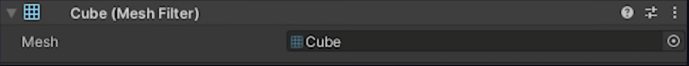
\includegraphics[width=1\linewidth]{chapters/14/Images/Mesh2.png}

\pagebreak

\subsubsection{Der Mesh Renderer}
Der Mesh Renderer ist dafür verantwortlich Materalien und Lichteffekte wie Reflextionen bei einem Objekt darzustellen.\\
\noindent
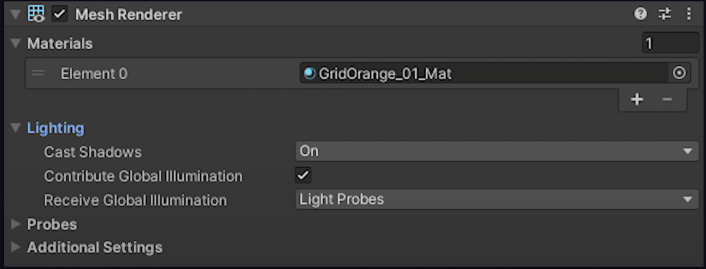
\includegraphics[width=0.7\linewidth]{chapters/14/Images/MeshRenderer.png}

\subsubsection{Die Physics Komponenten}
\glqq Adding a Rigidbody component to an object will put its motion under the control of Unity's physics engine. Even without adding any code, a Rigidbody object will be pulled downward by gravity and will react to collisions with incoming objects if the right Collider component is also present. \grqq \cite[][Rigidbody]{unitydocRigidbody} \\
\noindent
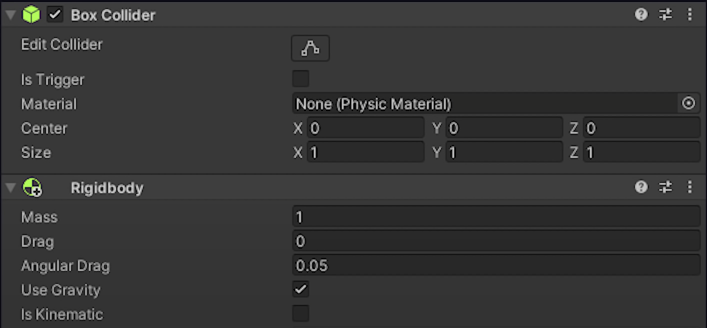
\includegraphics[width=0.7\linewidth]{chapters/14/Images/Physics.png}


\pagebreak
\setauthorname{Martin Usta}
\subsection{Skybox}\
Eine Skybox ist der Hintergrund unsere Spielewelt. Dabei is Skybox ist ein Würfel, indem sich unsere Spielewelt befindet. Die inneren Seiten des Würfels bilden unseren gesamten Hintergrund.
Zu beachten ist das die Würfelseiten die richtige Textur bekommen. Jede Seite hat seine eigene Koordinate für die vergebene Textur:\\\\

\begin{minipage}{0.4\textwidth}
    \begin{itemize}
        \item +Z für vorne 
        \item -Z für hinten 
        \item +X für links 
        \item -X für rechts
        \item +Y für oben
        \item -Y für unten
    \end{itemize}
  \end{minipage}
  \hfill
  \begin{minipage}{0.6\textwidth}
    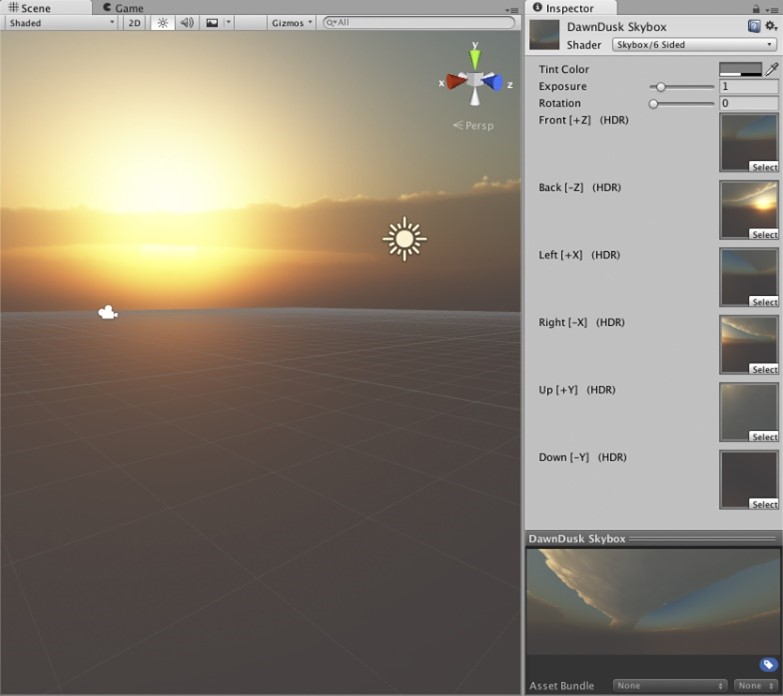
\includegraphics[width=\linewidth]{chapters/14/Images/Skybox.png}
  \end{minipage}

\pagebreak
\subsection{Animation}

Beim Animieren geht es darum, dem Nutzer eine scheinbare Bewegung des Spielobjekts zu vermitteln. Dabei werden die beweglichen Abläufe eines Spielobjekts erstellt und aufgenommen. Hierbei werden die Koordinaten bestimmter Körperelemente in Keyframes festgehalten. Diese können dann auf einer Zeitachse platziert werden. Dadurch wird ein Keyframe mit den gespeicherten Koordinaten zum entsprechenden Zeitpunkt aufgerufen, um eine Bewegung zu simulieren.
\pagebreak
\setauthorname{Martin Usta}
\chapter{Blender}

\subsection{Einführung}
Blender ist ein umfangreiches Programm für die Erstellung von 3D-Objekten. Diese Software kann man auch zum Animieren, Zeichnen, Video Editieren oder Ähnlichem benutzen. 
In dieser Diplomarbeit wird der Fokus auf den 3D-Viewport und auf die Animation gesetzt. Das sind die wichtigsten Funktionen für die weiter Bearbeitung in Unity. 

\subsection{3D-Viewport}
Im 3D Viewport kann man das 3D-Objekt bearbeiten. Für diese Bearbeitung hat die Software folgende Tools: 

\begin{itemize}
    \item \textbf{Objekt Mode}:
    \indent Das Objekt als gesamtes kann bewegt und bearbeitet werden. 
    \item \textbf{Edit Mode}:
    \indent Einzelne Kanten, Punkte und Oberflächen können von einem Objekt verändert werden. 
    \item \textbf{Sculpting Mode}:
    \indent Bei diesem Mode kann das Objekt dynamisch verändert werden.
    \item \textbf{Vertex Paint}:
    \indent Einzelne Ecken, Punkte und Oberflächen können in eine separate Gruppe zusammen gegliedert werden
    \item \textbf{Weight Paint}: 
    \indent Weight Paint ist dafür da, um zu bestimmen, wie abhängig ein Objekt zu einen Animationsskelet ist. 
    \item \textbf{Texture Paint}:
    \indent Diese Funktion dient zur Bemalung des Objektes.
\end{itemize}

\pagebreak

\subsection{Objekt Mode}

Im Objekt Mode können die Objekte verändert werden.
Dabei kann man, die Größe, die Länge und die Breite geändert werden.
Außerdem kann das Objekt rotiert und die Position im 3-dimensionalen Raum verändert werden. 
Es können zudem weitere Objekte hinzugefügt werden.
\begin{figure}[H]
    \centering
    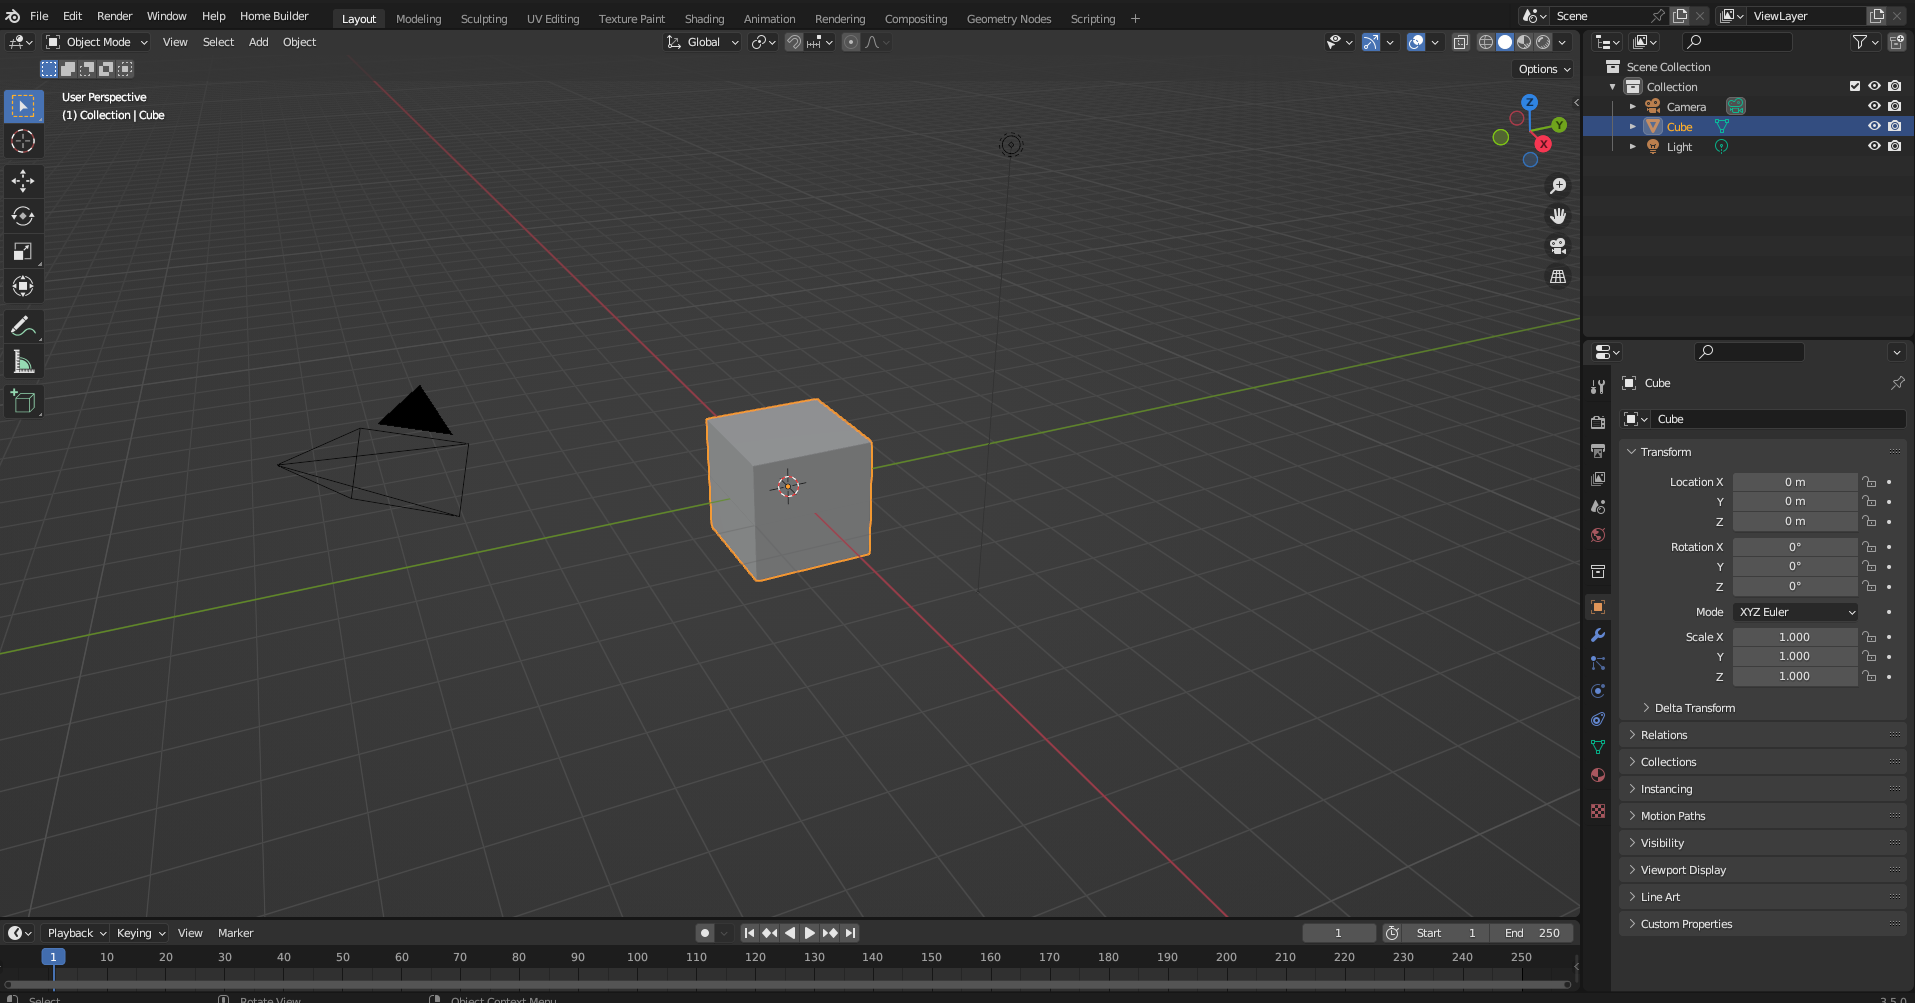
\includegraphics[width=0.8\textwidth]{chapters/13/images/3D-Viewport.png}
    \caption{Ein selectierter Würfel im Objekt Mode von Blender.}
    \label{UST-8}
\end{figure}


\subsection{Edit Mode}
Dieser Modus bietet eine Reihe von Tools, um die gewünschte Form des Objekts zu erzeugen.
Diese Tools sind:


\begin{itemize}
    \item \textbf{Extrudieren}:
    \indent Das Extrudieren wird verwendet , um eine Fläche höher oder tiefer zu ziehen und somit als neuer Würfel zu dem Objekt hinzuzufügen.
    \begin{figure}[H]
        \centering
        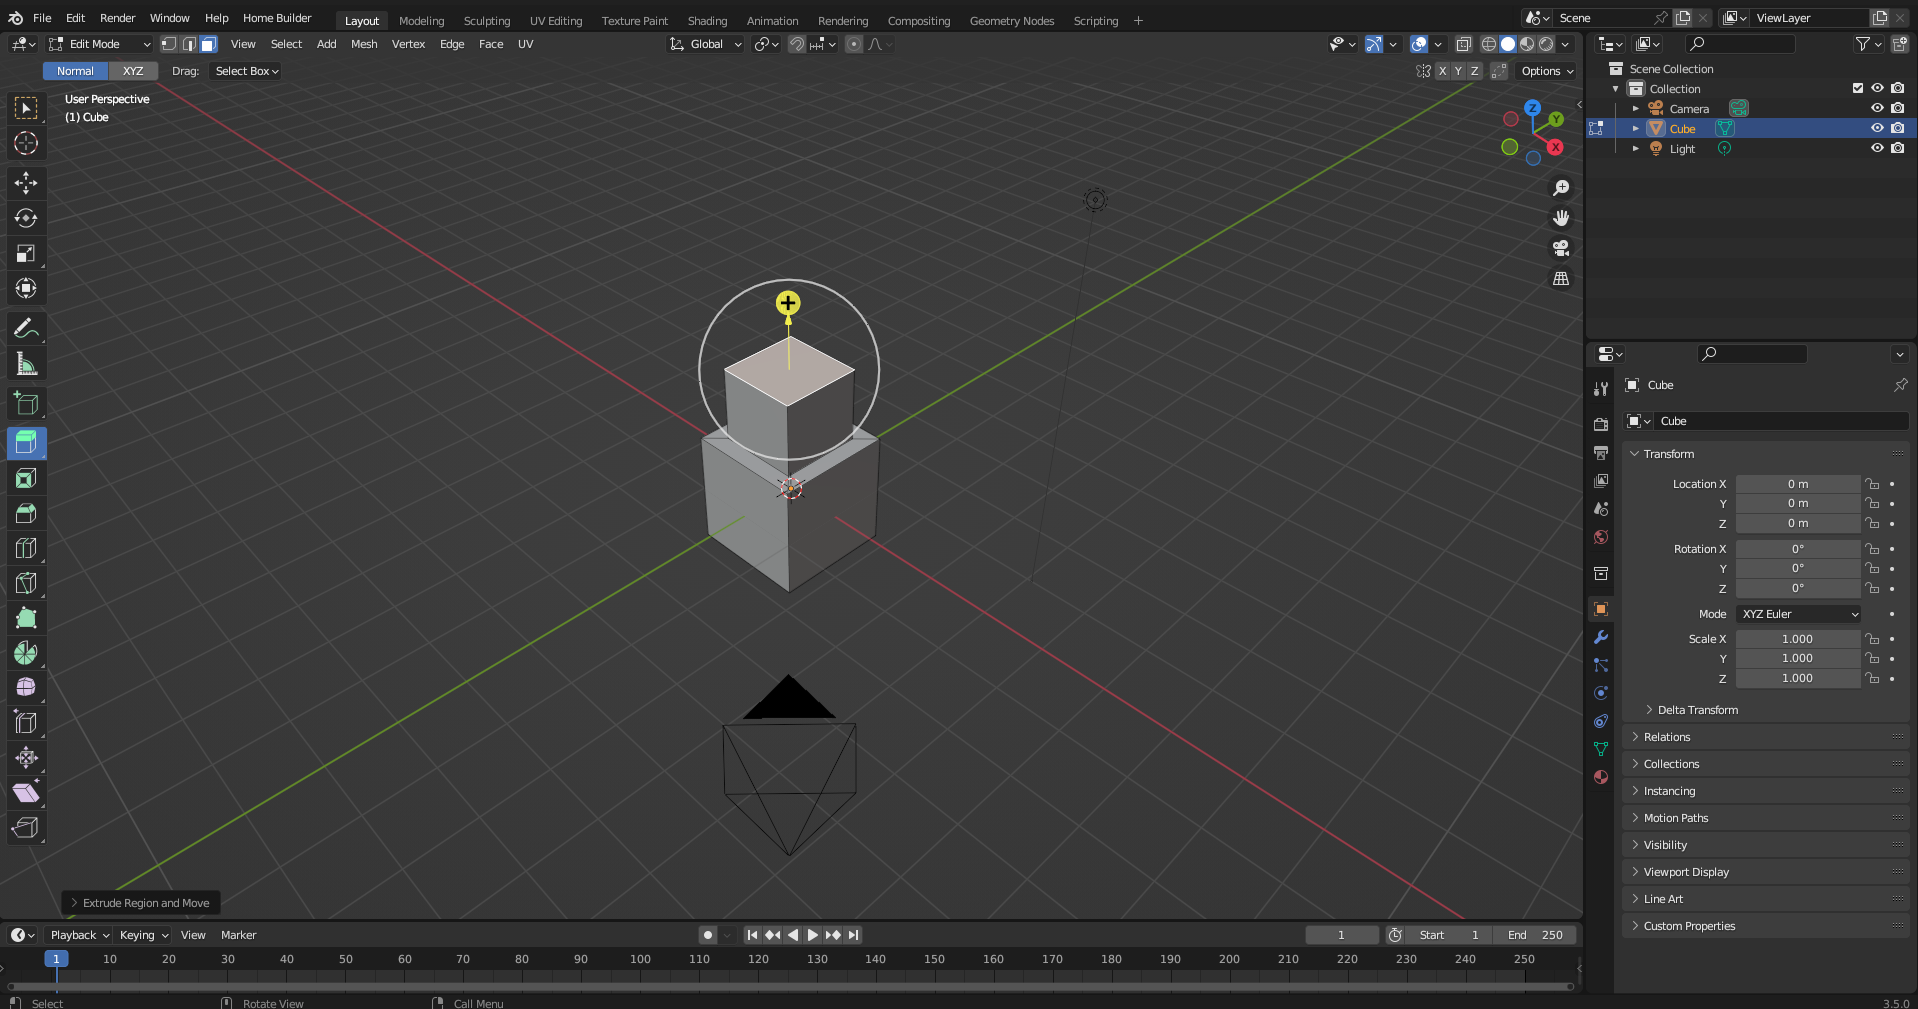
\includegraphics[width=0.8\textwidth]{chapters/13/images/ExtrudeTool.png}
        \caption{Eine Extration von einer Würfelfläche.}
        \label{UST-9}
    \end{figure}
    
    \item \textbf{Inset Faces}:
    \indent Das Inset Faces Tool ermöglicht das Erstellen von neuen Flächen innerhalb einer ausgewählten Fläche, was beispielsweise für die Erstellung von Löchern oder symmetrischen Auswuchtungen benötigt wird.
    \begin{figure}[H]
        \centering
        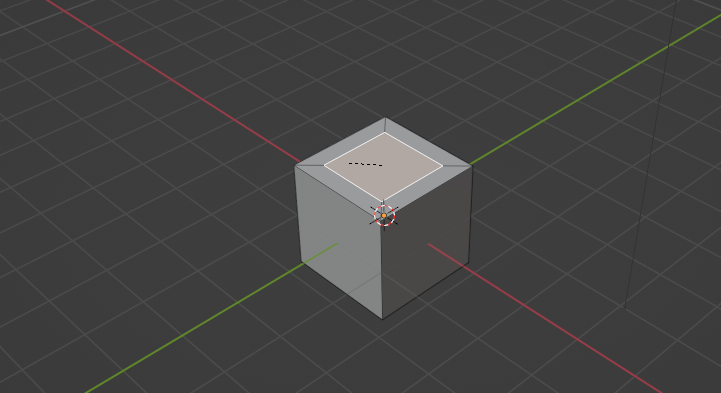
\includegraphics[width=0.8\textwidth]{chapters/13/images/InsetFace.png}
        \caption{Die Funktion Inset Faces erstellt eine neue Fläche auf einer ausgewählten Fläche.}
        \label{UST-10}
    \end{figure}
    
    \item \textbf{Loop Cut}:
    \indent Mit dem Loop Cut Tool können zusätzliche Kanten um das Objekt erstellt werden. Hiermit werden symmetrisch zum Objekt neue Kanten erstellt.
    \begin{figure}[H]
        \centering
        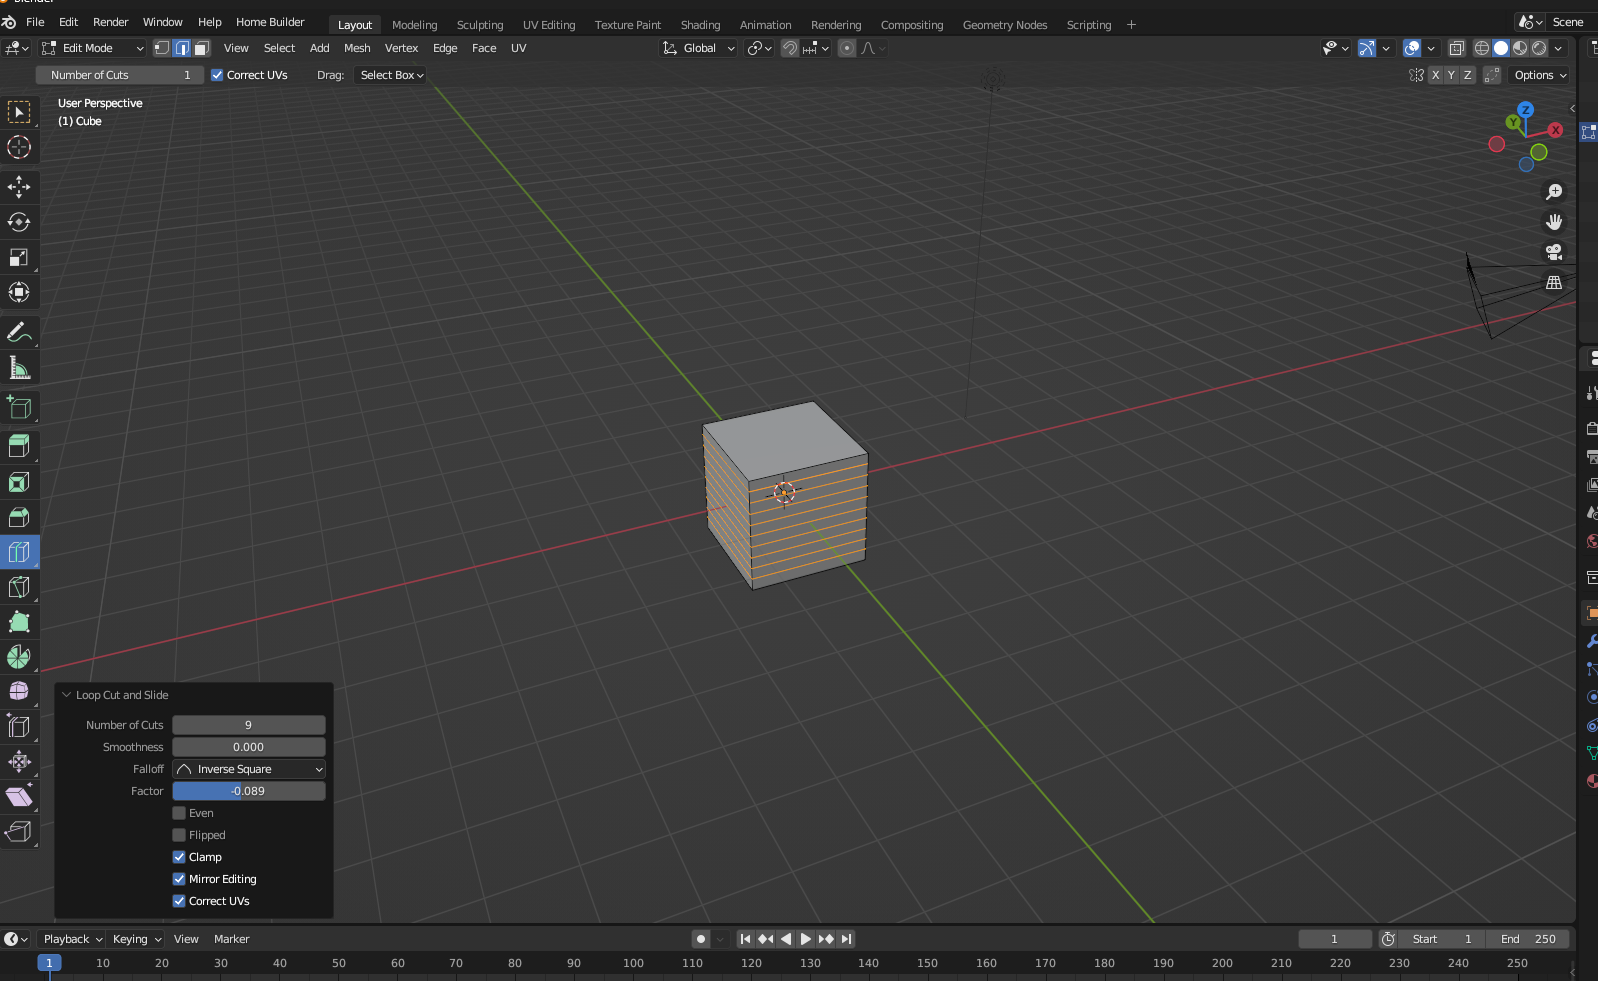
\includegraphics[width=0.8\textwidth]{chapters/13/images/Loopcut.png}
        \caption{Die Anwendung des Loopcut Tools wird auf einen Würfel verwendet.}
        \label{UST-11}
    \end{figure}
    \item \textbf{Messer}:
    \indent Das Messer Tool ermöglicht, Kanten mit der Freihand hinzuzufügen. Das wird benötigt, um Kanten an nicht symmetrischen Stellen zu erzeugen.
    \begin{figure}[H]
        \centering
        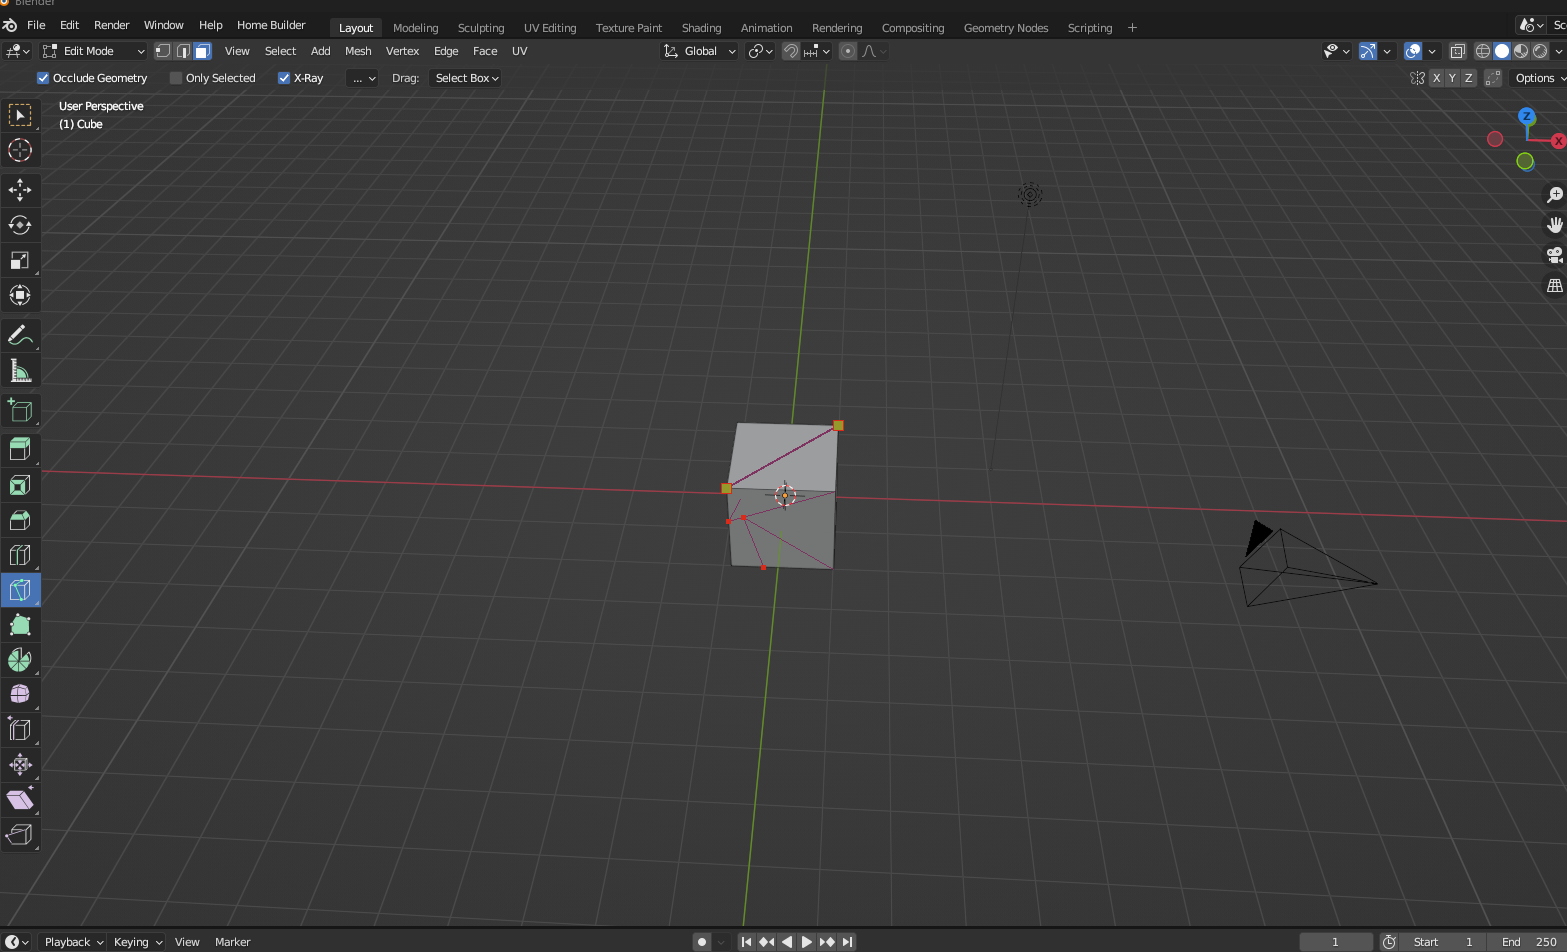
\includegraphics[width=0.8\textwidth]{chapters/13/images/KniveTool.png}
        \caption{Die Anwendung des Knive Tools wird auf einen Würfel verwendet.}
        \label{UST-12}
    \end{figure}
    \item \textbf{Poly Builder}: 
    \indent Schließlich bietet das Poly Builder Tool die Möglichkeit, einzelne Kanten zu markieren und die Länge zu verändern, um das Objekt nach Belieben zu verändern.
    \begin{figure}[H]
        \centering
        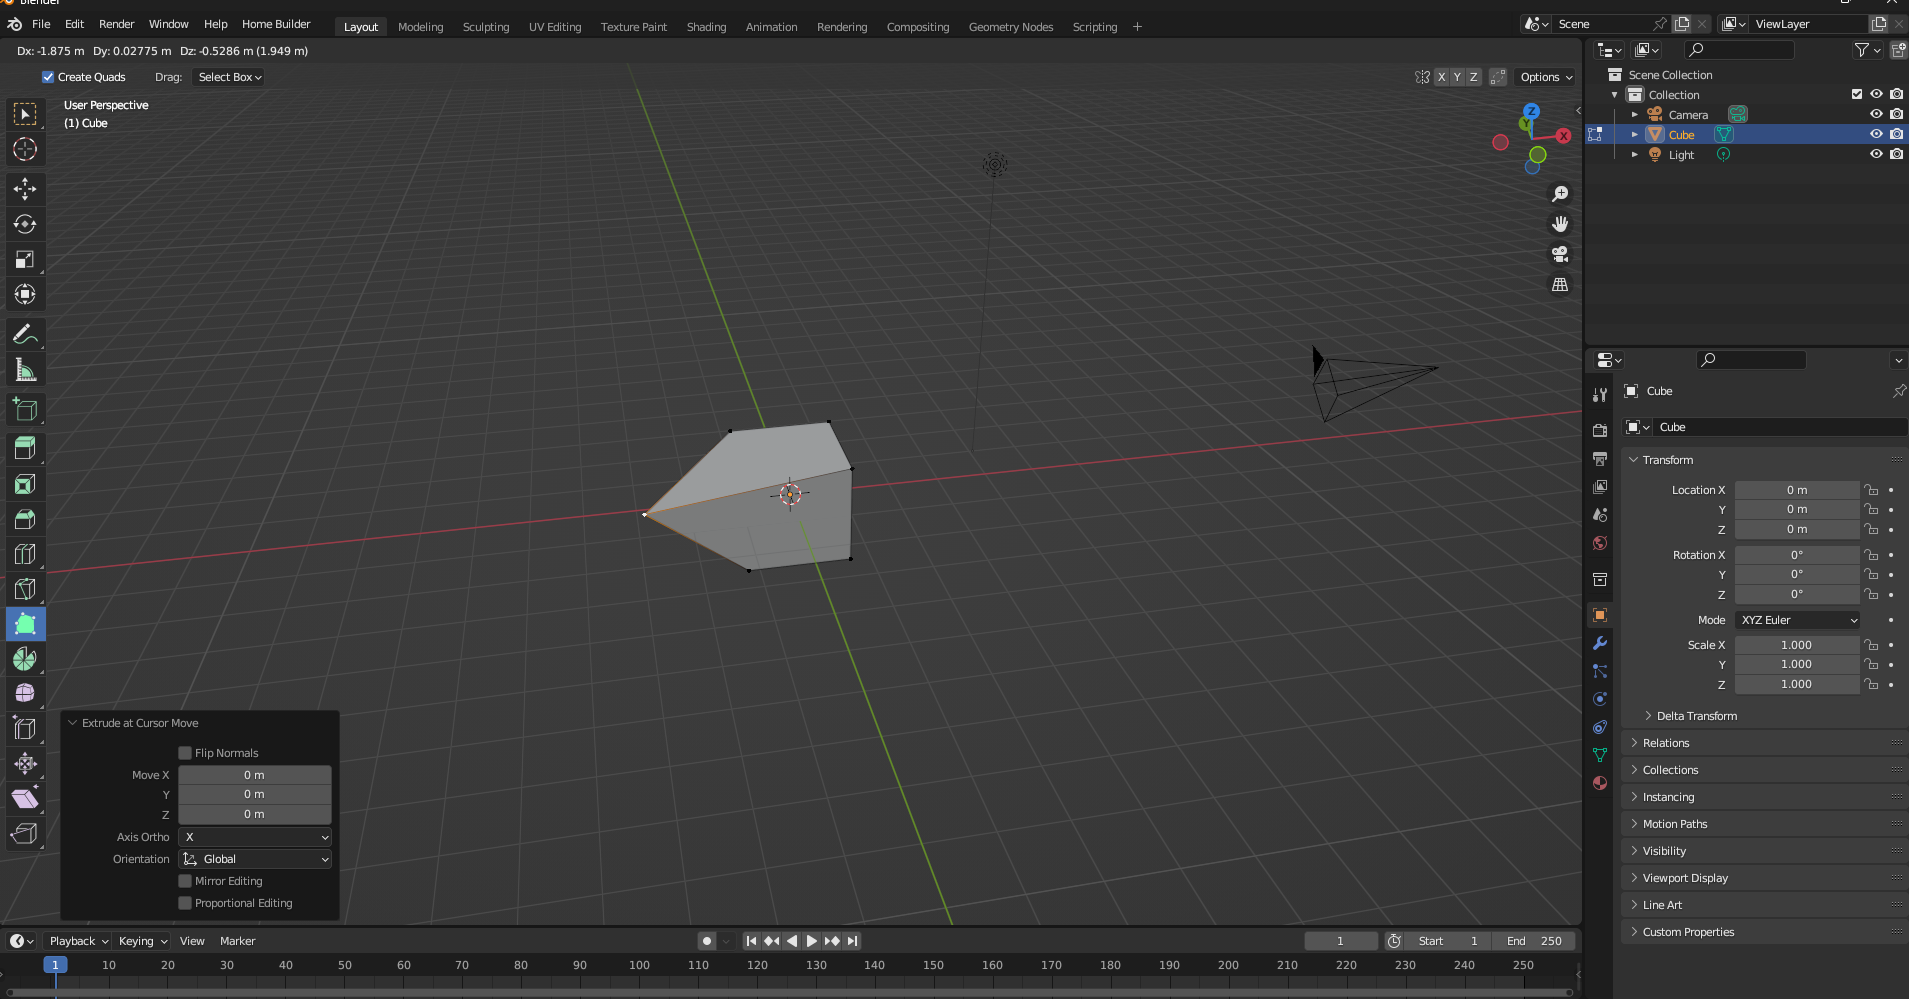
\includegraphics[width=0.8\textwidth]{chapters/13/images/PolyBuild.png}
        \caption{Die Anwendung des Poly Build Tools wird auf einen Würfel verwendet.}
        \label{UST-13}
    \end{figure}
\end{itemize}
%https://docs.blender.org/manual/en/latest/editors/3dview/modes.html

\subsection{Sculping Mode}
Der Sculping Mode hat verschiedene Tools um das Objekt dynamisch zu verändern. In diesem Tool kann die \bettergls{topology}{1} bearbeitet werden. Hier kann die Anzahl der Polygone wie im Edit Mode dynamisch verändert werden. Die Arbeitsweise in diesem Tool ist wie folgt.\\\\
Zuerst werden grobe Details des Objekt erzeugt wie zum Beispiel die Grundform des Objekt.\\\\
\begin{figure}[H]
    \centering
    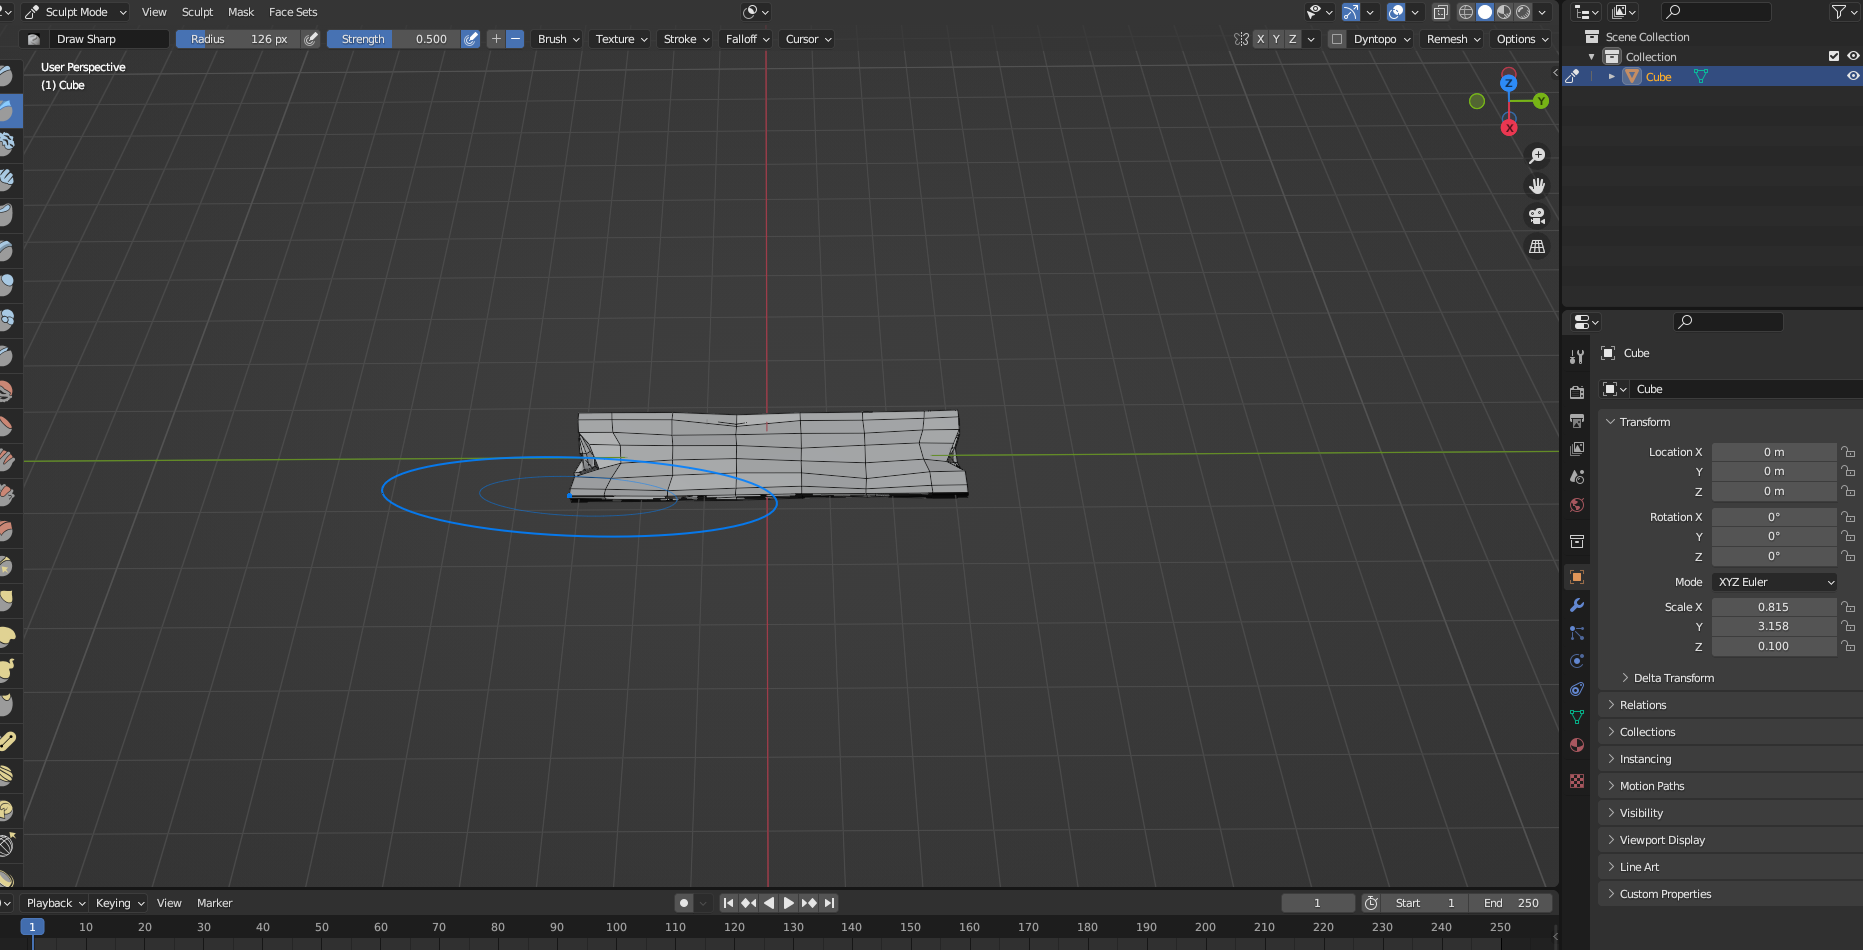
\includegraphics[width=0.8\textwidth]{chapters/13/images/HolzBrett.png}
    \caption{Die Bearbeitung der Grundform eines Spielobjekts®.}
    \label{UST-14}
\end{figure}
\noindent Danach wird die Anzahl der Polygone erhöht um feinere Details hinzuzufügen. Dieser Workflow dient dazu so immer auf einer Detailstufe zu bleiben.
\begin{figure}[H]
    \centering
    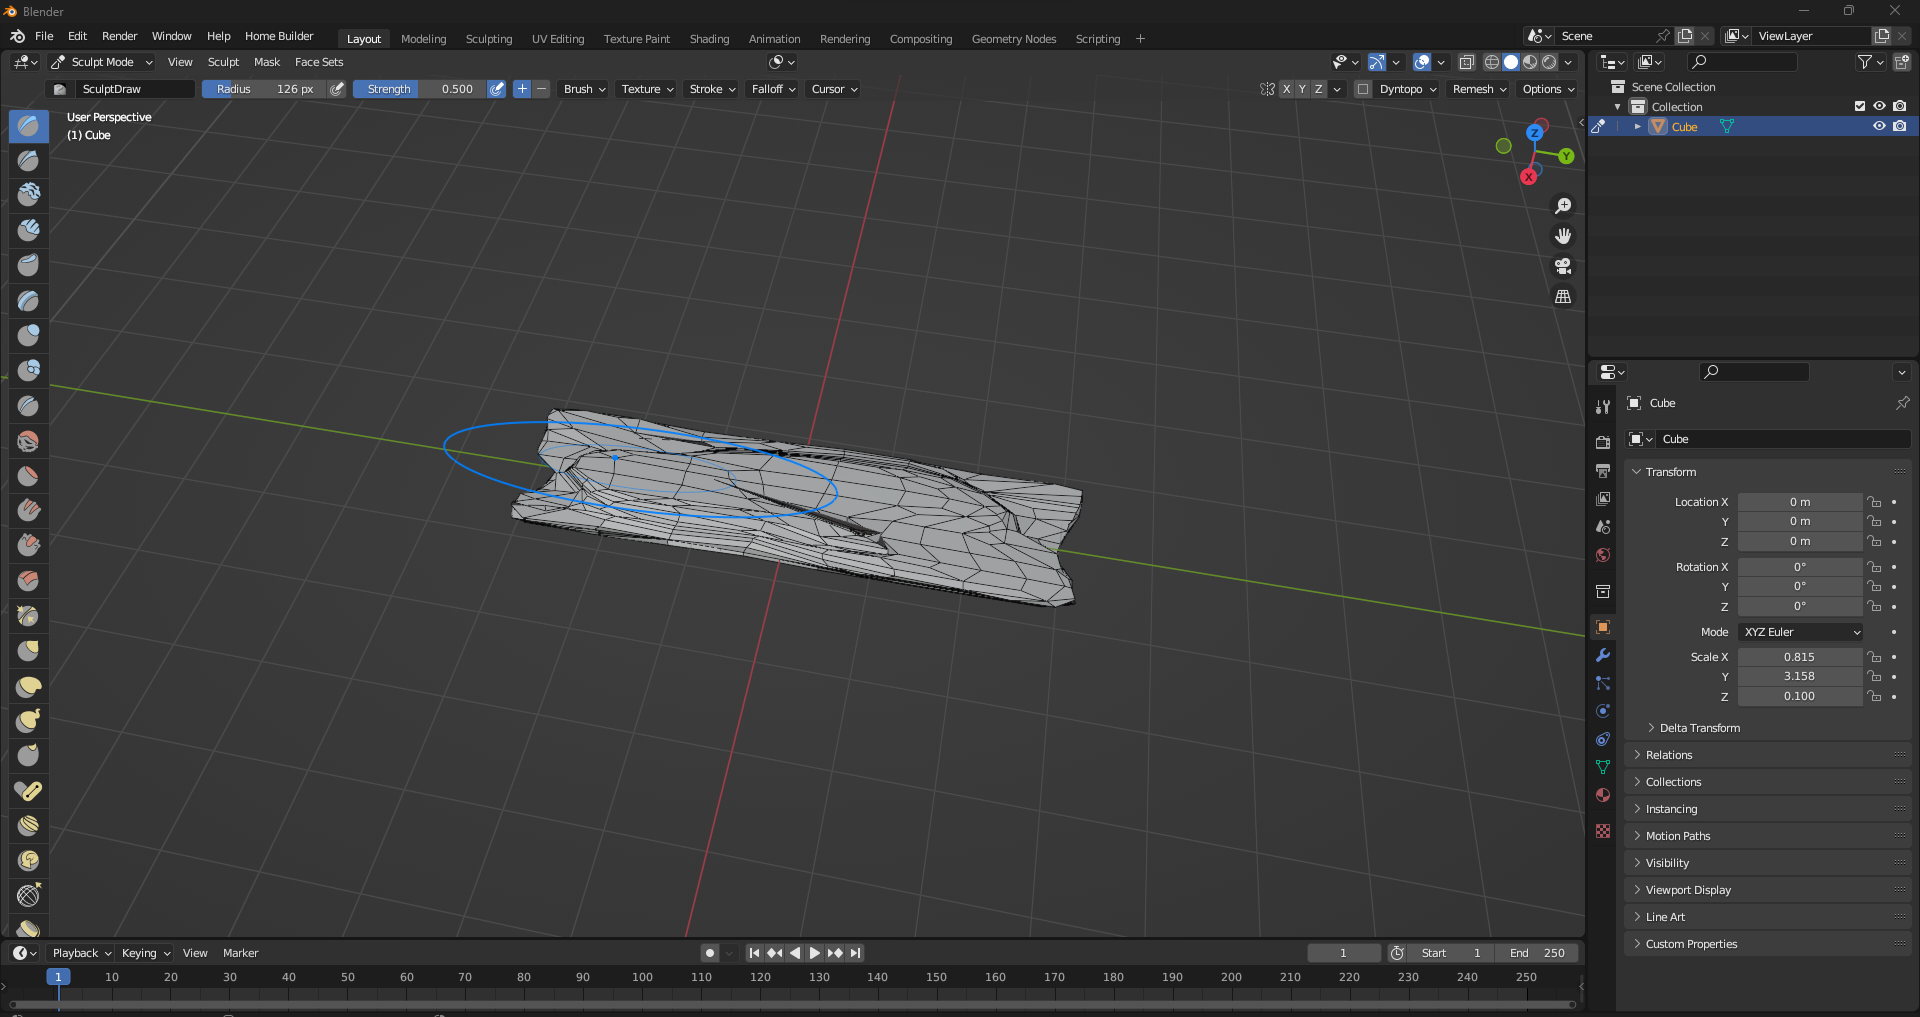
\includegraphics[width=0.8\textwidth]{chapters/13/images/HolzBrett1.png}
    \caption{Die Bearbeitung gröberer Details mit einer höheren Polygonanzahl.}
    \label{UST-15}
\end{figure}
\noindent Dieser Ablauf wird 2 bis 3 mal wiederholt um ein schönes detailiertes Objekt zu erstellen.
\begin{figure}[H]
    \centering
    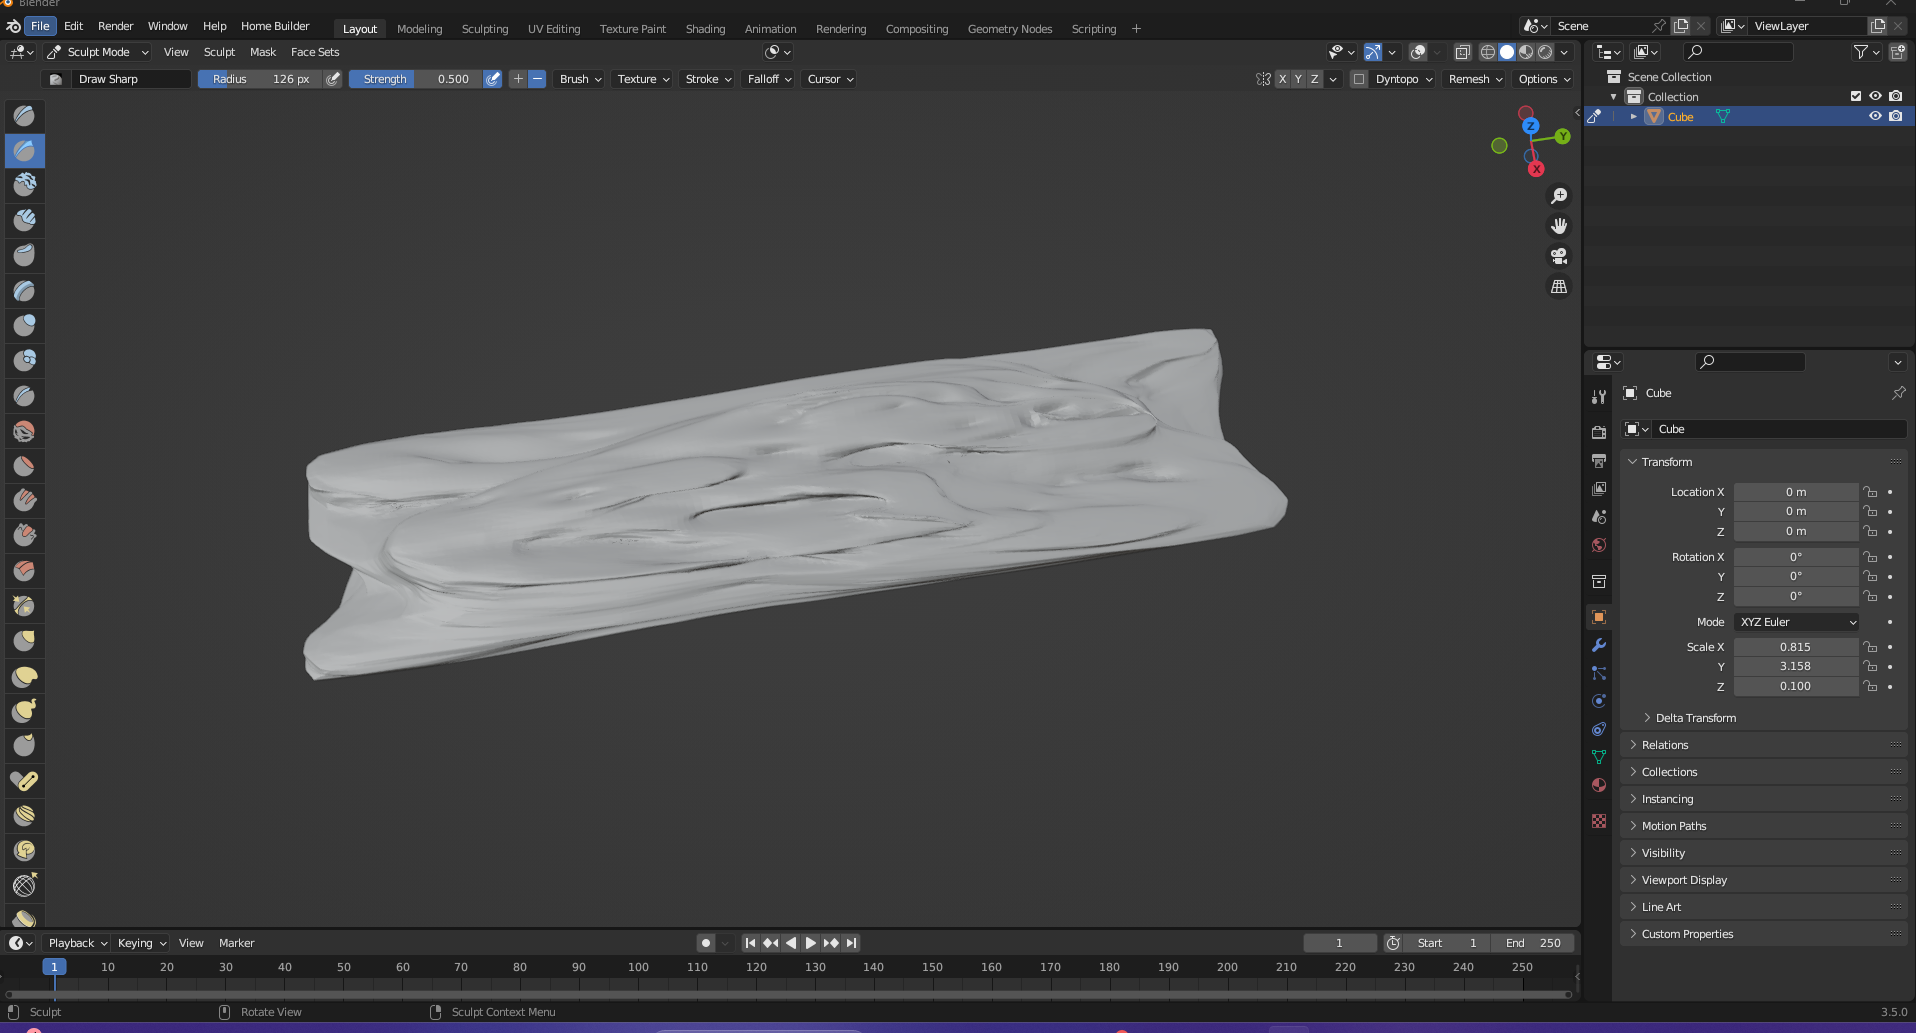
\includegraphics[width=0.8\textwidth]{chapters/13/images/HolzBrett2.png}
    \caption{Die Bearbeitung feinere Details auf das Objekt.}
    \label{UST-16}
\end{figure}
\noindent Wichtig ist darauf zu achten, dass je mehr Polygone das Objekt besitzt desto mehr muss die Cpu rechnen. Das kann zum weiteren, zur schlechteren Performance im Spiel verusachen. Der letzte Schritt ist dann wieder das Runterskalieren der Objekte. Dieser Schritt ist wichtig um unnötige Polygone nicht zu laden. Wichtig dabei ist, dass die Details bebehalten werden.Um das zu gewährleisten, werden Bereiche des Obejekt runter skaliert. In der Folgenden Abbildung kann man erkennen, dass die orange Fläche keine Details enthält und somit runterskaliert wurde.

\begin{figure}[H]
    \centering
    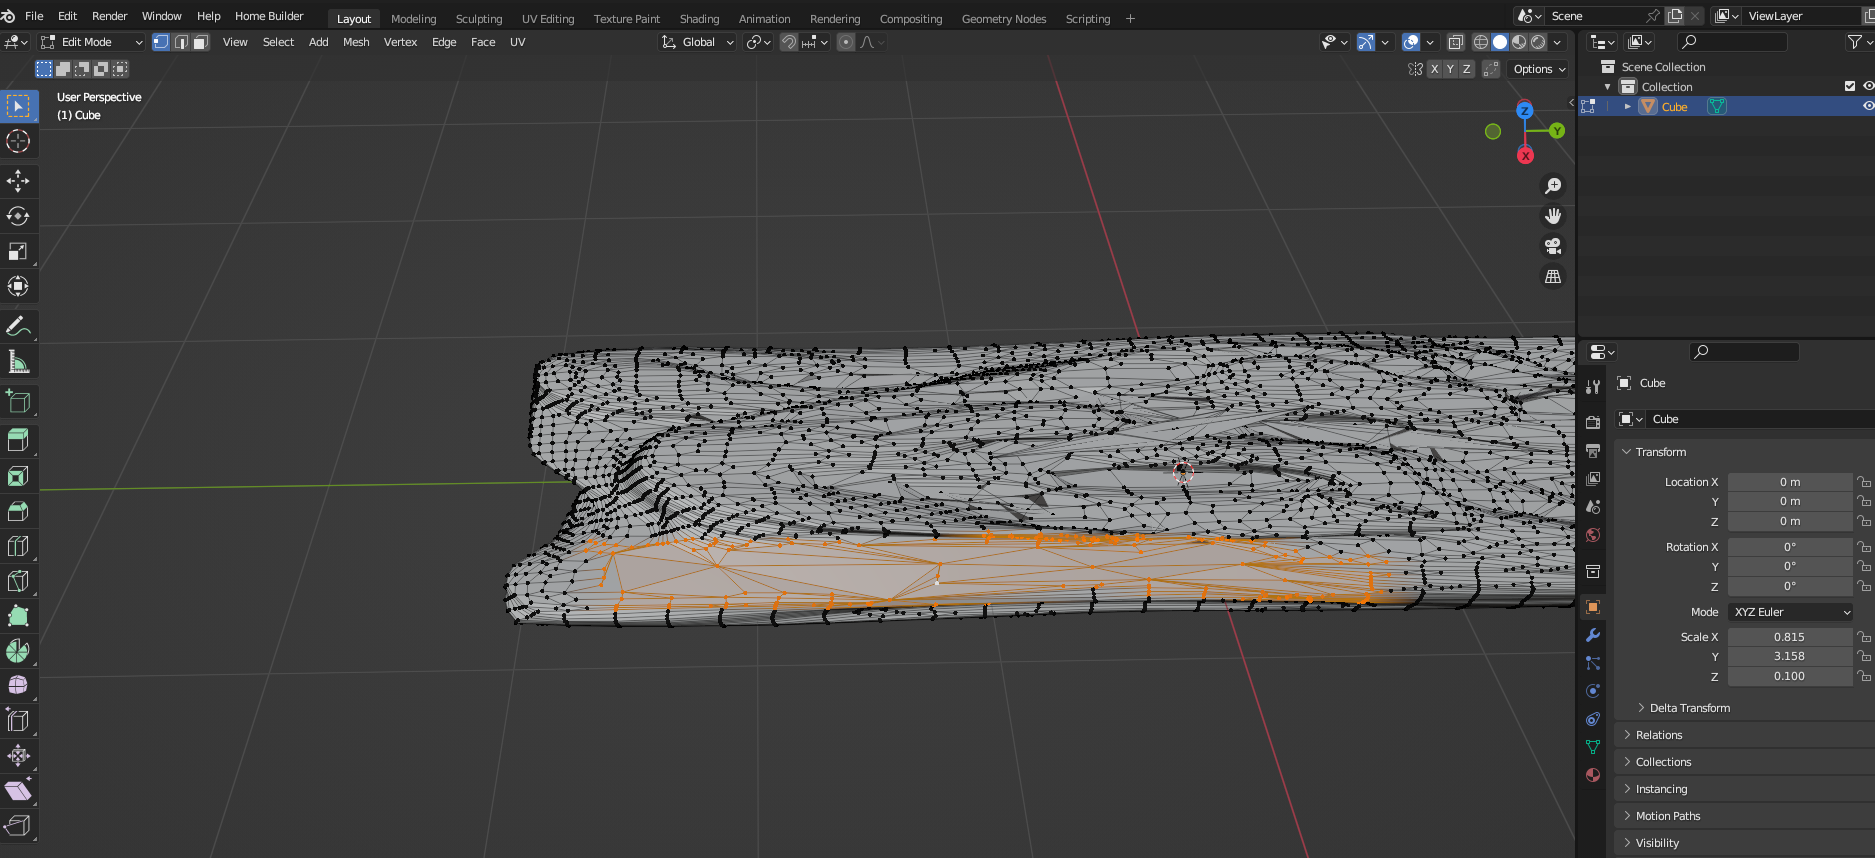
\includegraphics[width=0.8\textwidth]{chapters/13/images/HolzBrett3.png}
    \caption{Die runterskalierung einer bestimmten Fläche auf dem Objekt.}
    \label{UST-17}
\end{figure}


\pagebreak
\setauthorname{Martin Usta}
\chapter{Spieleperformance}


\subsection{Einführung}
In jedem Spiel ist es wichtig, dass das Spiel ohne Performanceverluste funktioniert. Die Performance wird von der Spielewelt und ihren Spielobjekten beeinträchtigt. Bei der Spielentwicklung muss sehr oft abgewogen werden ob bestimmte Details ins Spiel implementiert sein müssen. Denn jedes noch so kleine Detail braucht Rechenleistung. In der Spieleentwicklung werden nur selten Spielobjekte wegen des Leistungsverlustes entfernt. Meistens werden diese für das Spiel optimiert.Bei der Spieleentwicklung kann man die Performance anhand von zwei Faktoren optimieren. Ein Faktor betrifft dabei die Spiel-Engine, während der andere Faktor das Modellierungsprogramm betrifft.. %todo: fix text grammar

\subsection{Spielobjekt Optimierung im Grafikprogramm}
Bei den Grafikprogrammen kann vieles gemacht werden um das Spielobjekt performance effizienter zumachen. Wenn ein Gameobjekt erstellt wird, besteht dieses aus Seiten und Flächen. Diese werden auch Polygone genannt. Die Polygon Anzahl bestimmt den Detailgrad des Spielobjekts, das heißt je mehr Polygone das Objekt besitzt desto detailreicher ist es. Wenn ein Objekt viele Polygone besitzt, kann es sein das die Performance im Spiel darunter leidet. Denn sobald sich ein Polygon in der Darstellungsdistanz befindet, wird es berechnet. Um die Anzahl der Polygone niedrig zu halten, werden die Details als "Objekt-Images" gezeichnet. \\\\ %todo: change the ****
Bei dem ersten Prototypen entstand das Problem, dass mehrere Spielobjekte zu viele Polygone hatten. Somit mussten wir die meisten Objekte in unseren Prototypen neu bearbeiten. Dieser Vorgang wird auch als 'Mapping' bezeichnet. %todo: fix the ""
\pagebreak
\subsection{Objekt Mapping}

Bei einem Objekt-Image handelt es sich um ein Bild, welches über das Objekt gelegt wird. Für dieses Verfahren muss erst das Objekt für das Bild \verb+unwrapped+ werden. Dieser Vorgang zerlegt das Objekt in sogenannten Maps.\\\\
In der nächsten Abbildung wird auf der linken Seite eine \verb+unwrapped+ Map von einem Stein gezeigt, der in unseren Prototypen implementiert wird. Auf der rechten Seite ist das 3D-Objekt abgebildet.


\begin{figure}[H]
    \centering
    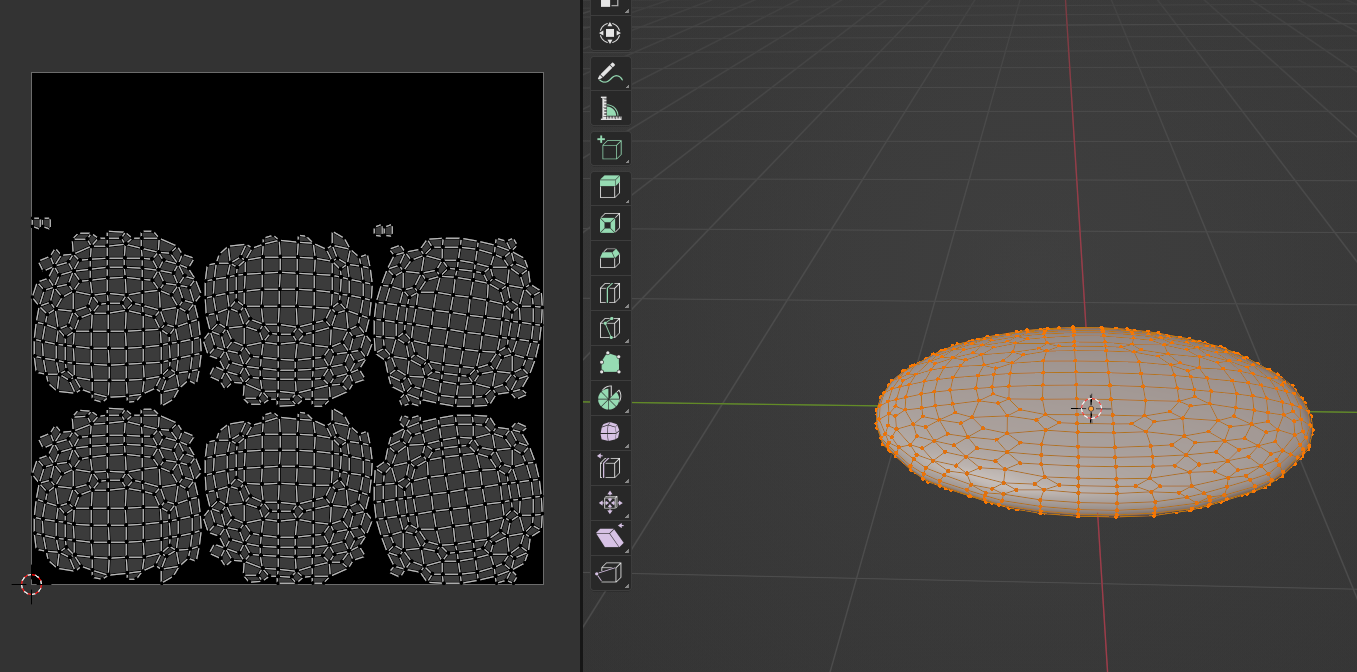
\includegraphics[width=0.8\textwidth]{chapters/11/Images/StoneAndUnwrap.png}
    \caption{Eine Abbildung einer unwrapped map und des Objektes.}
    \label{htl01}
\end{figure}

\noindent Nun könnte man ein Bild unter das entfaltete Mapping legen und damit weiterarbeiten. Auf diesem Bild können nun sämtliche Details eingezeichnet werden. Sobald die Details eingezeichnet wurden, wird das Bild "gebacken". Im folgenden Bild sieht man das Objektbild eines Steins: %todo: maybe rewrite this

\begin{figure}[H]
    \centering
    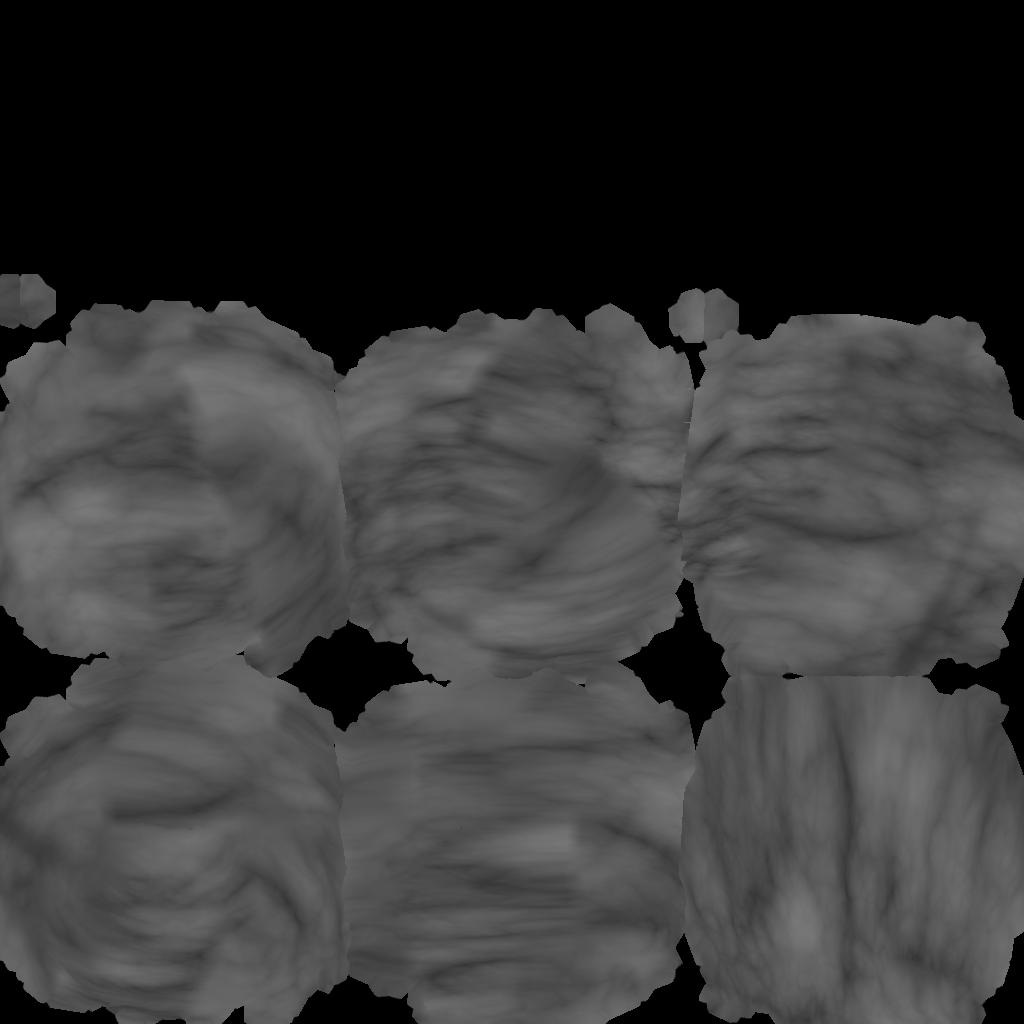
\includegraphics[width=0.4\textwidth]{chapters/11/Images/SteinColor.png}
    \caption{Eine Abbildung einer Colormap des Objektes.}
    \label{htl01}
\end{figure}

\subsection{Normal Maps}

Normal-Maps sind Images, die die Eigenschaft besitzen Höhen und Tiefen eines Objektes aufzunehmen. Diese werden auch verwendet, um dem Objekt eine simulierte Höhe und Tiefe zu geben. Bei dem folgendem Bild wird eine Normal-Map von einem Stein gezeigt.

\begin{figure}[H]
    \centering
    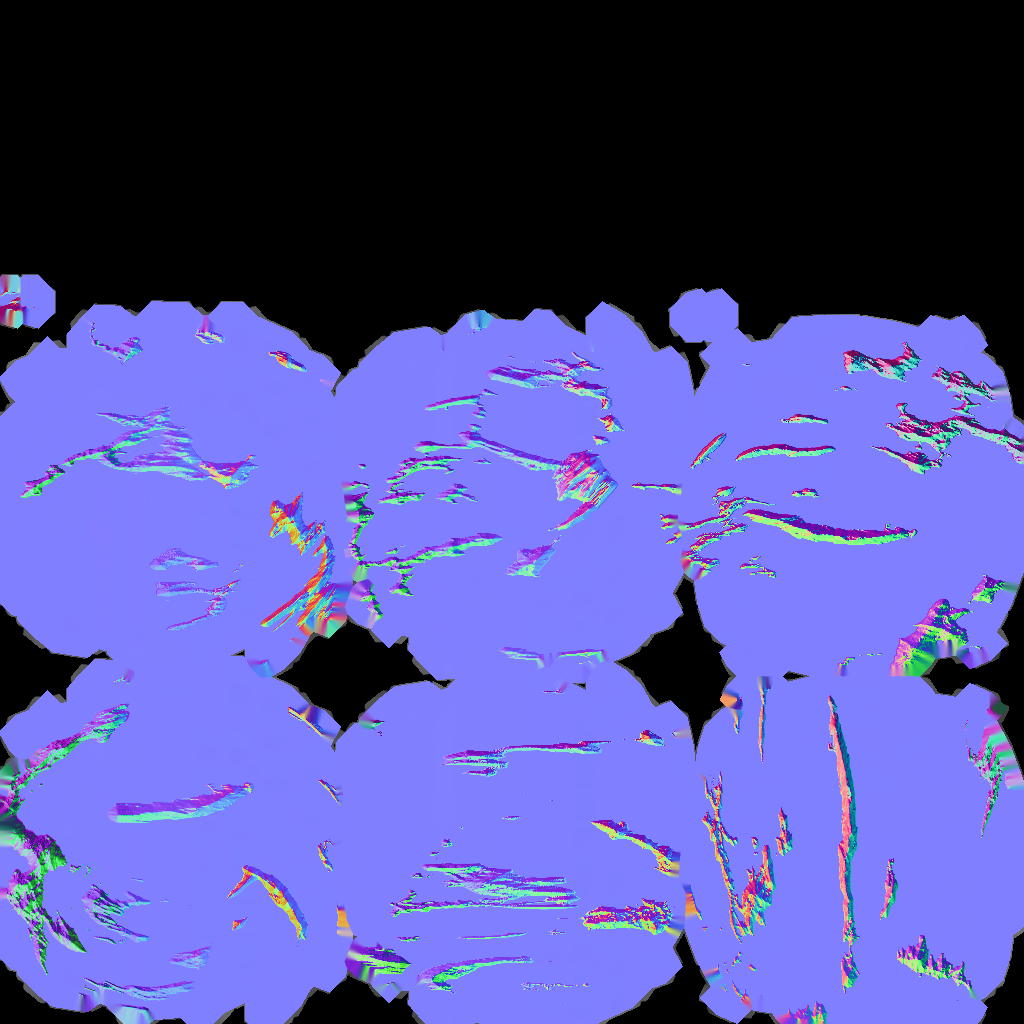
\includegraphics[width=0.4\textwidth]{chapters/11/Images/SteinNormal.png}
    \caption{Eine Abbildung einer Normalmap des Objektes.}
    \label{htl01}
\end{figure}
%todo: abbildung ist highlightet weil ich das geändert habe und das man nachher aufpassen muss dass die nummer stimmt
\noindent Bei der Normal-Map von der \hl{Abbildung 7.3} ist deutlich zu erkennen, dass der blaue Bereich die flache Fläche darstellt, während die farblichen Striche hingegen Kratzer zeigen, welche der Stein beinhaltet.

\subsection{Maps Kombinieren}

Als letzten Schritt müssen alle Maps kombiniert werden. Diese werden in dem Grafikprogramm übereinandergelegt.\\\\
Das Endresultat zeigt den Stein mit einer geringe Polygonanzahl aber mit einer großen Vielfalt an Details. In der nächsten Abbildung wird das Endresultat des Steines gezeigt.

\begin{figure}[H]
    \centering
    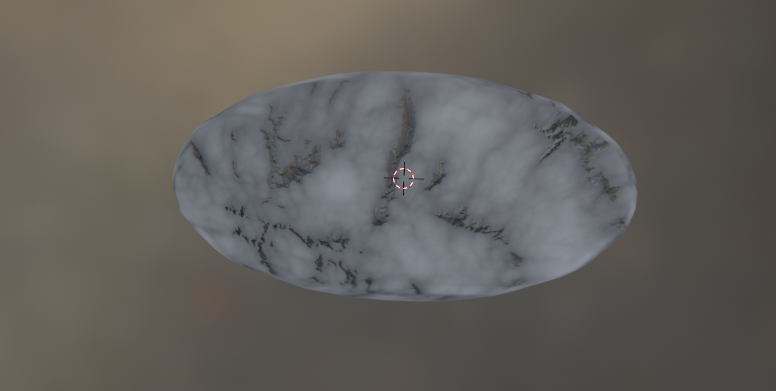
\includegraphics[width=0.6\textwidth]{chapters/11/Images/SteinCombi.png}
    \caption{Eine Abbildung des fertigen Objektes.}
    \label{htl01}
\end{figure}

Um das Objekt in Unity zu implementieren, werden alle Maps in Unity gebraucht. Es ist auch wichtig zu bedenken, dass Unity ein anderes Koordinatensystem hat als Blender. Somit muss beim Export die richtige Richtung angegeben werden. Sonst kann es passieren, dass das Objekt in Unity in eine andere Richtung zeigt.

\begin{figure}[H]
    \centering
    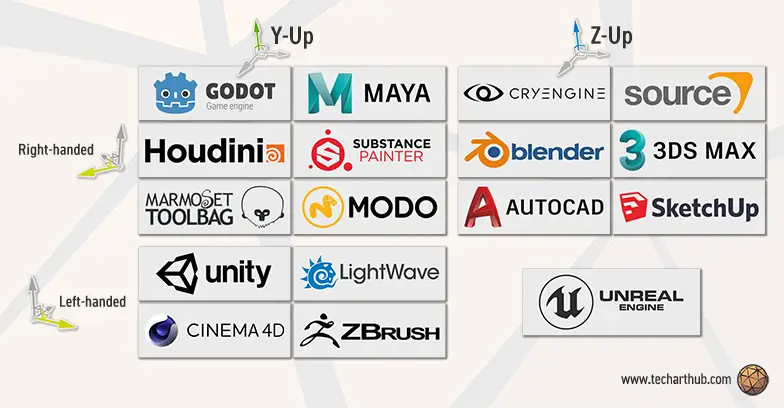
\includegraphics[width=0.6\textwidth]{chapters/11/Images/Koordinaten.png}
    \caption{Eine Abbildung unterschiedlicher Programme und deren Koordinatensystemen}
    \label{htl01}
\end{figure}

\pagebreak
\pagebreak
\setauthorname{Martin Usta}
\chapter{Spieledesign} % todo: maybe fix überschrifteneinheitlichkeit
\section{Spieledesign} % todo: spieledesign/spieldesign 

Das Spieldesign umfasst mehrere Gebiete der Spielentwicklung. Die verschiedenen Gebiete des Spieldesign sind:

\begin{itemize} % todo: überschriften überarbeiten?
    \item Level Design - Umgebungsdesign 
    \item Theme Auswahl 
    \item Spiel Schwierigkeit 
    \item Musik
\end{itemize}

Bei diesen Gebieten der Spielentwicklung ist es wichtig, dass sie das selbe Theme verfolgen und zueinander passen. Falls die Gebiete des \hl{Spiels-design} nicht zueinander passen, so wird das \hl{Spiele-Erlebnis} für den \hl{Endkonsumenten schlecht}. 

\subsection{Leveldesign - Umgebungsdesign}
Das Leveldesign besteht aus zwei voneinander abhängigen Gebieten. \hl{Das betrifft das Level und die Umgebung die es betrifft.} Dabei geht es beim Leveldesign um: Spielfiguren, Plattformen, Levelaufbau, Levelphysik etc. 
Das Umgebungsdesign befasst sich mit der Umgebung des Spiels wie zum Beispiel: Himmel(Skybox), Berge, Flüssigkeiten, Sonneneinstrahlung, etc. 
Beide Aspekte entscheiden wie realistisch das Spiel auf den Spieler wirkt. Es ist nicht zum Empfehlen den Grafikstyle zwischen den Properties und der Umgebung zu mischen.

Ein Level besteht immer aus statischen Objekte und dynamischen Objekte. %todo: maybe insert citation?

\pagebreak

\subsection{Statische Objekte} %todo: footnote einheitlich machen
Statische Objekte sind Spielelemente die keine Interaktionsmöglichkeit für den Spieler bieten. Sie dienen meisten als Prop\footnote[1]{ist ein Spielobjekt} welches als nicht bewegliches Levelobjekt zählt. \\\\
Ein statisches Objekt könnte zum Beispiel ein Bücherregal in einem Level sein. Dieses bietet dem Spieler keine Interaktionsmöglichkeiten sondern dient nur der Ästhetik des Raumes. \\

\hl{
    Ein weiteres Beispiel wären Häuser die im Spiel implementiert sind, diese sind meist als ortgebundenes Objekt in der Welt, welches nur den Sinn hat, als Location für das nexte Spielevent zu dienen. Auch Objekte die nur den Sinn haben die Welt lebhafter zu gestalten wie Bäume, Fässer, Steine usw. dienen nur also Dekoelement. Diese dienen nur als optische Bereicherung für das Level. 
}

\subsection{Dynamische Objekte}
Dynamische Objekte haben im Gegensatz zu statischen Objekten eine \hl{Programmierung || maybe passt 'Funktion' besser} im Hintergrund. Diese Objekte haben einen aktiven Einfluss auf das Spielgeschehen. Zudem können sie mit dem spielbaren Charakter interagieren. Hier muss aber wieder differenziert werden zwischen Umgebungsobjekt und NPC(non playable character).\\\\ % todo: footnote for npc + bibliotek eintrag
Ein Umgebungsobjekt wäre zum Beispiel eine Platform die sich bewegt. Diese hat einen aktiven Einfluss auf den Spieler. Meistens werden dynamische Umgebungsobjekte als Herausforderung dem Spieler entgegengestellt. Ein Beispiel wäre eine Falle, die den Spieler blockiert bis dieser einen versteckten Schalter findet. \hl{
    Die Anwendung für Umgebungsobjekte sind grenzenlos. %todo: maybe useless sentence
}\\\\
Ein NPC(non playable character) zählt zwar auch als dynamische Objekt aber hat einen anderen Nutzen als das Umgebungsobjekt.Ein NPC muss nicht ein Gegner sein dieser kann den Spielbaren Charakter helfen. Eine Rolle wäre die eines Questgebers, dieser kann den Spieler ein Aufgabe geben, die dieser erfüllen muss um weiter im Spiel voranzuschreiten. Eine andere Tätigkeit ist ,dass der Spieler von einem NPC blockiert werden kann oder sogar den Spieler angreift um ihn zu besiegen.

\pagebreak

\section{Die Spielewelt}
In einem Spiel gibt es immer eine Spielewelt in der die Geschichte erzählt wird. Diese kann aus mehreren kleinen Leveln bestehen oder nur einem großen Level. In der Gamingbranche wird solches auch als Openworld bezeichnet.


\subsection {Sektionale Level}
Ein sektionalen Level besteht aus mehreren Level und Szenen. er große Vorteil ist, dass Assets in einem anderen Level wiederverwertet werden können. weiteres ist,dass die Level unaphängig voneinander sind. Somit können größere Storysprünge gemacht werden. Der Nachteil dabei ist, dass der Storyfluss unter anderem gestört wird falls die Sprünge zwischen den Level zu groß sind. 

\subsubsection{Spielobjekte in sektionalen Leveln}
In eine sektionalen Level sind die Spielobjekte nicht an die anderen Level gebunden. Somit können die Assets je nach Level komplett unterschiedlich sein. Nehmen wir das beispiel von dem Klassiker Super Mario 64. Hierbei ist ein Level sommerlich gestaltet und das nächste im Winterdesign. Zudem können dann im weiteren Spielverlauf Spielobjekte wiederverwendet werden. Die wiederverwendet Objekte werden nur wenig verändert, damit diese zum Leveltheme passen. Was auch Interessannt ist, die Tatsache auch Gegenerische Spielfiguren nur leicht verändert werden um deren Stärke zu Demostrieren. Zum Beispiel der Videospiel Klassiker Chicken Invaders. Bei diesem Spiel habe die Gegnerischen Spielfiguren das gleiche Model nur die Farbe der tragenen T-Shirts verändert sich. Zum Beispiel haltet ein Huhn mit einen Roten T-Shirt weniger aus als Eins mit Blauen usw. Hier bei wird eindeutig nur die Farbe geändert und somit viel Zeit ersparrt für das Designen neuer Gegner. 

\section{Openworld}
Die Openworld ist eine Spielewelt, die keinen Level wechsel besitzt. Somit spielt die gesamte Geschicht in einem Level. Das Level bei einer Openworld ist um das Vielfache größer als eine sektionales Level. Im Gegensatz zum sektionale Spieledesign besteht die Openworld aus zusammengesetzten Level.   


\subsection{Spielobjekte in einer Openworld}
In einer Openworld sind die die Spieleobjekte vom Designaspekt abhängig. Die Objekte einer Openworld sollten die ganze Zeit zusammenpassen, sonst wirkt es unpassend und das Spielerlebnis wird gestört. Wenn wir uns die Openworld von GTA 5, 2013 anschauen sieht man, dass diese sehr durchdacht. In der Stadt sind Wolkenkratzer, Autobahne, Geschäfte usw. Im Gegensatz wenn man in den Wald geht, da sind Tiere, Holzfällerhütten, Bäume usw. Wichtig ist, dass der Übergang zwischen den unterschiedlichen Gebieten schön übergehen. 

\todo{die letzten zwei absätze lies dir durch ab hier hab ich nicht weitergelesen}

\subsection{Kamera und Sichten}
In einer Spielewelt gibt es immer eine Kamera, die das Spielgeschehen den User auch anzeigt. Diese kann sowohl statisch auf eine Szene im Spiel plaziert sein, als auch auf die Spielfigur selbst. Zum Beispiel wäre es bei einem Schachspiel essentiell das sich die Kamera nicht bewegt und die Linze auf das Spielbrett zeigt. Indesem fall währe die Sicht die Adlereperspektive auch Dropdown genannt. Hier zeigt die Kamera von Oben nach Unten.Dann gibt es noch unterschiede zwischen den sichten wie die Spielfigur gezeigt wird. Da wären folgende:

\begin{itemize}
    \item \textbf{First Person:}
    \noindent Die firtsperson Sicht zeigt die Sicht aus der Spielfigur
    \item \textbf{Third Person:}
    \noindent Die thirdperson Sicht zeigt sowohl die Spielfigur als auch alles runterum. 
\end{itemize}

\subsection{Theme Auswahl}
Das Theme bestimmt welche Atmosphäre das Spiel haben soll. Bei dem Theme ist es wichtig das es mit dem Gameplay abgestimmt ist. Es gibt viele Arten von Themes von Horror bis zum Abenteuer ist alles dabei. Nach der Theme Auswahl kann die Planung für die  Game Assets beginnen. Zudem entscheidet das Theme weitere Spieldesign Aspekte: wie die Musik, die Spielmechaniken und die  Story. Wir haben uns für ein Fantasie Theme entschieden. Das heißt das die Grafik sehr bunt gestaltet ist und einen nicht realistischen Grafikstil. Bei einen Fantasie Theme ist die Auswahl der Gestaltung des Levels sehr umfangreich. 


\subsection{Spiel Schwierigkeit}

Bei der Spieleentwicklung ist es wichtig die Schwierigkeit des Spieles zu bestimmen. Schwierigkeit bestimmt den Flow des Spielverlaufs. Die Schwierigkeit sollte je nach Zielgruppe abgestimmt werden. Für die Spieler ist es wichtig, dass das man gefordert wird. Das gibt den User das Gefühl etwas erreicht zu haben. Zudem sollte das Spiel nicht zu schwer sein, damit der Spieler nicht frustriert wird. 

%https://www.nuclino.com/articles/level-design#:~:text=What%20is%20level%20design%3F,player%20and%20keep%20them%20engaged.

\pagebreak
\setauthorname{Martin Usta}
\chapter {Story und Theme}

\subsection{Einführung}
In diesem Kaptitel geht es um die Überlegung und Planung des Themes und der Story.Die Story auch übersetzt Geschichte genannt ist die Handlung die während des Spiel geschehen erzählt wird. Das Theme stärkt das Spiel geschehen, indem visuelle und audiodive Spielelemente die Story kräftigt. Bei der Theme Auswahl ist es wichtig, dass diese von der Story bestimmt wird. Das heißt wenn die Story fröhlich ist wird das Theme bunter sein, aber wenn die Story eine taurige Geschichte erzählt, wird das Theme düsterer. 

\subsection{Die Story}
Die Story soll den Spieler während des Aufenthalts in der Spielewelt unterhalten. Die Story kann sowohl fiktiv sein oder realistisch. Ein gutes Beispiel für ein Spiel mit einer realistischen Story ist Assasin Screed. Dieses Spiel erzählt viel über die vergangenheit. Da zählt dazu wie Davinci seine ersten Erfindungen greirt bis zu dem Unabhängigkeitstag von Amerika. Doch die meisten Spiele befinden sich in einer fiktiven Welt. Das hat den Grund, weil viele Menschen gerne etwas neues sehen wollen. Es ist wie ein neues Buch lesen mit einer komplett neuen Handlung. Weiteres sollte die Story auch mit dem Entwicklerteam abgesprochen werden. Der Grund dafür ist, dass die Theme gestaltung sonst sehr unpassend zur ist. 



\subsection{Story telling}

Beim Story telling geht es darum wie die Geschichte in einem Spiel den Spieler nahe gebracht wird. Es gibt viele Ansätze aber es gibt zwei Hauptstrategien, die die heutige Spieleindustrie verwendet. Das eine wäre die environmental Storytelling und indexcial Storytelling. In dem Artikel \citetitle{Fernadez1} vom \citeauthor{Fernadez1} im Jahr \citeyear{Fernadez1} wird beschrieben die Vor- und Nachteile beider Methoden.Hierbei schrieb der Author \citeauthor{Fernadez1} über das Besprochene in dem Diskurs von der  \citefield{Fernadez1}{journaltitle}.Dabei werden manche Aussagen folgender Entwickler zetiert und Analysiert (Carson, 2000; Pearce, 2007; Rouse, 2010; Smith and Worch, 2010). .In diesem Kapitel werde ich genauer erläutern was genau diese Methoden machen und wann welche eingesetzt wird. 

\subsection*{Environmental Storytelling}
Bei environmental Storytelling, wird die Geschichte von der Umwelt erzählt.Der Spieler nimmt daher die Rolle eines Besuchers ein beziehungsweise einen passiven Aktör in der Handlung. Jedes Ereignis, welches passiert, ist vordefiniert und wird sich nicht ändern. Dabei Spielen die Entscheidungen, welcher der Spieler macht keine Rolle. Der Vorteil an dieser Methode ist, dass sich der Spieler komplett auf die Handlung des Spiels konzentireren kann.Dabei folgt der Spieler einen linearen Weg der Story. Der Nachteil dabei ist, dass sowohl die Story, das Story telling und das Theme miteinander perfekt synagieren müssen. Zudem gibt environmental Storytelling keine Informationen wie das Spiel funktioniert. Somit muss sich der Spieler selber mit der Steurung befassen. Es sollte nie die Spielewelt mit der echten Welt interagieren.

\subsection{Indexcial Storytelling}
Bei indexcial Storytelling wird die Geschichte von Aktionen und Reaktionen des Spielers bestimmt. Hierbei verändert sich die Welt aufgrund des Spielers. in diesem Verfahren ist der Spieler ein aktiven Glied in der Story. Ein Beispiel welches \Citeauthor{Fernadez1} erwähnte wäre ein Taktik Shooter wobei der Spieler entscheiden kann ober alle Gegner besiegt oder keinen erledigt um an das Ziel zukommen. Hier hat eindeutig der Spieler mehr Freiraumum um das Spielgeschehen.\\\\
Aber auch die Story kann komplett anderst erzählt werden als in der environmental Storytelling. Auch ein gutes Beispiel vom dem Artikel \citetitle{Fernadez1} war Portal. Hier wurde die Geschichte was vor dem Zervall des Labors von einen Verrückten wissenschaftler auf die Wände gezeichnet. Sowas nennt man auch Story bites. Dabei wird die Story von Ereignis zu Ereignis erzählt und immer nur in kleinen Stücken.
\begin{figure}[H]
    \centering
    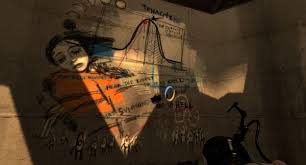
\includegraphics[width=0.6\textwidth]{chapters/15/images/Portal.png}
    \caption{Eine Grafik von dem beschrieben Portal Grafitti.}
    \label{UST-6}
\end{figure}
Im Gegensatz zu environmental Stortelling darf das indexcial Storytelling mit dem Spieler agieren. Das bedeutet, dass das Spiel ihm helfen kann weiter zukommen in dem es den Spieler Tipps gibt. Die Steuerung kann auch durch ein Tutorial im Spiel erklärt werden.Aber auch durch Schilder oder Bücher die im Spiel verteilt sind können Storyinhalte besitzen.Ein gutes Beispiel wäre Super Mario 64 in dem der Spieler am Anfang ein Schild sieht, worin die Story als auch die Spielsteuerung erklährt wird. Wichtig ist, bei der Methode das es nicht das Spielerlebnis durch zu viele Interaktionen mit dem Spieler verschlechtert. 

\subsection{Spannung einer Handlung}
Die Handlung eines Spiel sollte immer spannend gehalten werden. Aber der den Spieler nie überfordern. Wenn der Spieler überfordert ist, ist dieser genervt und wie vielleicht nicht mehr das Spiel spielen. Aber die Story sollte auch nicht zu langweilig sein um das Spielerlebnis zu trüben. Zudem sollte die Handlung eines Spiel wie einen Film gleichen. Damit ist gemeint, das es am Anfang einen Aufbau der Story gibt. Danach bleibt die Steigung anhaltend bis am Schluss wo jeder Plot aufgelöst wird. Dieses verfahren wird in fast jeden literarischen Werk verwendet, ob es Film, ein Buch oder sogar ein Theater Stück. Dieses Schema ist beliebt da es Spannung erzeugt und den Endverbraucher (Spieler, Leser, Zuschauer) and die Geschichte klammert. 

\subsection{Spannung Gameplay}
Auch das \bettergls{gameplay}{1} muss eine gewisse Spannung habung. Wenn das Spiel zu leicht ist fühlt sich der Spieler unterfordert. Aber wenn das Spiel zu schwer ist er frustriert.\\\\
Wichtig ist das der \bettergls{flow}{2} optimal zum Spiel passt. Gehen davon aus es ist ein Spiel für jüngere verbraucher dann darf das Spiel nicht zu schwer sein da die Erfahrung mit Spielen einfach zu wenig vorhanden ist. Aber wenn Zielgruppe Personen sind die sich mit Videospielen gut auskennen, dann sollten sie auch Herausgefordert werden. Damit sie nicht während des Spielens aufgrund des zu leichten Gameplay keine lust mehr bekommen das Spiel zu spielen. Wichtig ist aber, dass der Flow während des Spielverlaufs ändert. Am Anfang sollte das Spiel einfach gehalten sein. Damit der User einen leichten Start in das Spiel bekommt. Wenn sich der Spieler an die \bettergls{gamemechaniken}{3} gewöhnt hat, muss der Spieler mehr gefordert werden damit sein Interesse bleibt. Zudem fuhlt sich das Spiel eintönig and wenn immer die gleiche Herausforderung entgegen kommt. In der folgenden Abbildung aus dem Buch \citetitle{GameDesign} kann man erkennen der Flow sich während des Spiels veränder soll.

\begin{figure}[H]
    \centering
    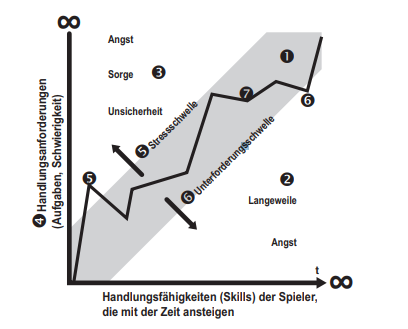
\includegraphics[width=0.8\textwidth]{chapters/15/images/GameFlow.png}
    \caption{Eine Grafik die den Flow verlauf des Spiels zeigt.}
    \label{UST-4}
\end{figure}


\subsection{Theme}
Das Theme ist dafür zuständig um die visuellen und audiodiven Reize des Spielers zu begeistern. Eine gute Story macht es nicht automatisch zu einem guten Spiel. Das Theme muss zur Story passen. In einem fröhlichen Spiel sind die Farben meist bunt und die Hintergrund-Musik sehr fröhlich und aufmundert. Nicht wie bei einer düsteren beziehungsweise trarigen Story, da werden ehe dunklere Farben und eine langsame umklammertende Musik verwendet. Das Theme muss den Spieler stimmig für die Story machen.

\subsection{Spielidee für den Prototypen}
Für den Prototypen habe wir (Martin Usta und Lukas Schachinger) uns entschieden das wir einen \bettergls{platformer}{4} machen. Dieser Sollte beinhalten Sammelobjekte in Form von Münzen. Aber auch schwierige Passage wo der Spieler sich gefordert fühlt. Der Spielbare Charakter sollte aufjeden fall dynamische Animationen besitzen. Zudem sollten auch Gegner in diesem Spiel vorkommen um den Spieler zuhindern das Ende zu erreichen. Die Inspiration für diese Art vom Spiel, war das damalige Kult Spiel \verb+Kao the Kangaro Round 2+ welches im Jahr 2004 im November erschiene ist.\\\\

\subsection{Storyline für den Prototypen}
Unser Hautprotagonist "generischer Name" ist eingeschlaffen und findet sich in eine Traumwelt als Eule wieder. Dieser versucht alles um dieser Welt zu entkommen. Doch diese Aufgabe ist schwieriger als er es vermuten mag. Um dieses Ziel zu beweltigen muss dieser Fallen ausweichen, Rätsel lösen und Gegener die ihm in den Weg stellen ausschalten. Dafür setzt er seine Eulenfähigkeiten ein. Ob in das gelingen wird ist nur eine Frage der Zeit. Aber er weiß er muss so schnell wie möglich aufstehen um sein Kind vom Kindergarten abzuholen. %todo: generischer name?

\begin{figure}[H]
    \centering
    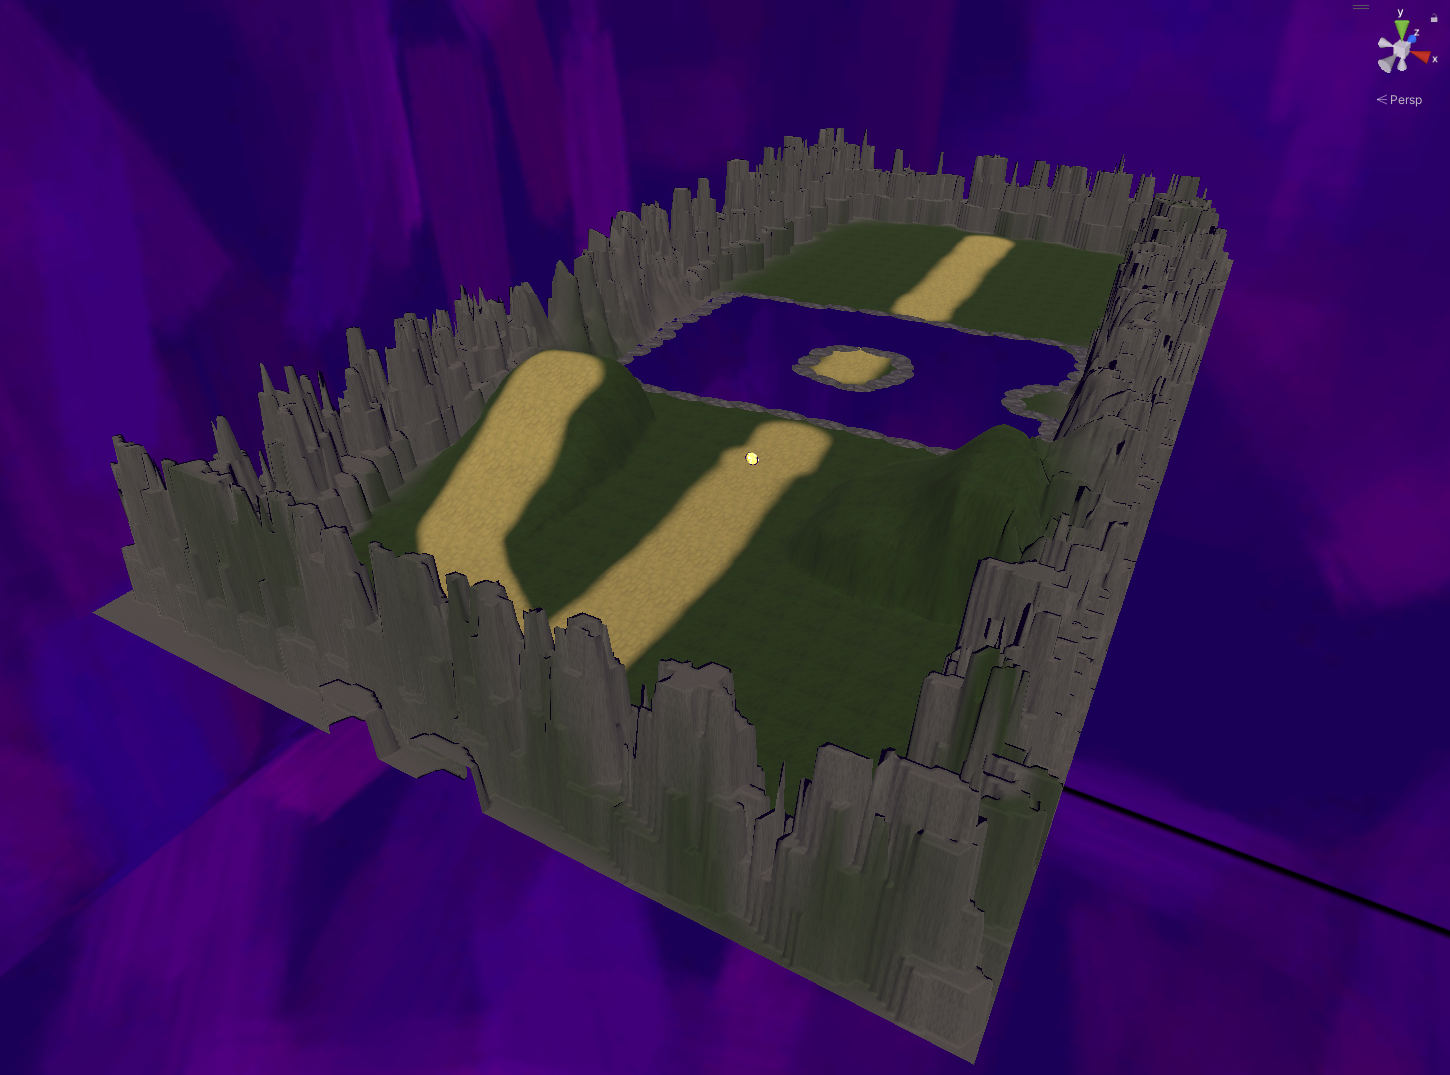
\includegraphics[width=0.8\textwidth]{chapters/15/images/Dreamworld.png}
    \caption{Eine Grafik des ersten Konzepts unsere Traumwelt.}
    \label{UST-7}
\end{figure}



\setauthorname{Lukas Schachinger}

\chapter{User Interface (UI) und Interaktion}

\begin{quote}
\emph{\glqq Im Interface begegnet der Spieler dem Spiel. [...] Die Schnittstelle zwischen Mensch und Computer/Konsole etc.\grqq}~\cite[][Game Design und Produktion: Grundlagen, Anwendungen und Beispiele; p.~161]{GameDesign} \\ 
\end{quote}

Das \bettergls{UI}{1} im Spieldesign ist fast der wichtigste Teil der Spielentwicklung, wenn man das Design des eigentlichen Spieles außen vornimmt. Ohne eine gute Menüführung und ein gut entworfenes User Interface ist es schwer, dass Spielerinnen und Spieler das Spiel verstehen und spielen können. 

\begin{figure}[H]
  \centering
  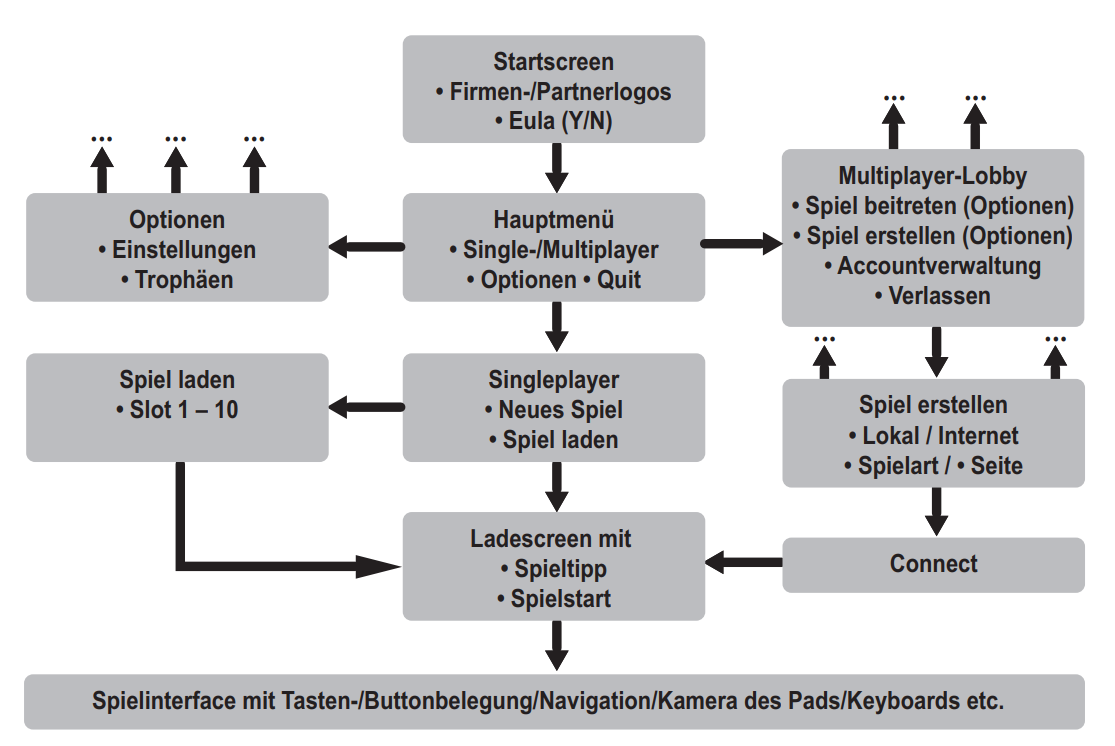
\includegraphics[width=0.6\textwidth]{chapters/03/images/Spielinterface.png}
  \caption{Ein Beispiel eines Dialogbaumes von einem Computerspiel.}
  \label{htl01}
\end{figure}

Der abgebildete Dialogbaum zeigt die verschiedenen Menüs und Screens die ein Computerspiel haben kann. Diese unterscheiden sich in den unterschiedlichen Arten von Spielen. Bei einem \bettergls{multiplayer}{2}-Spiel soll die Möglichkeit geboten werden, ein Spiel zu erstellen oder einem beizutreten. Während es bei einem \bettergls{singleplayer}{3} wichtig ist, Spielstände speichern und laden zu können.

\pagebreak

Das User Interface des Prototyps unterteilt sich in drei verschiedene Aspekte:

\begin{itemize}
    \item Hauptmenü
    \item User Interface während des Spieles
    \item Pausemenü
\end{itemize}

\noindent
Bei der Entscheidung, welche Komplexität das User Interface des Prototyps haben soll, fiel die Wahl auf ein simples Design. 
Das User Interface soll einerseits die Schlichtheit des eigentlichen Spieles wiederspiegeln und andererseits alle für das Spiel wichtigen Informationen darstellen.

\section{Gestaltung des Hauptmenüs}

Im Folgenden wird das Gestalten der Benutzeroberfläche für das Hauptmenü erläutert. 
Das Hauptmenü in der Spielentwicklung ist vergleichbar mit einem Türvorleger vor einer Haustür. Es soll das Willkommenschild für das eigentliche Spiel sein. 
Mithilfe dieses ersten Eindrucks ist es möglich zu erkennen, um welche Art von Spiel es sich handelt. Das \bettergls{theme}{1} des Spieles spiegelt sich in dem Design des Hintergrundes und in der Schriftart des Hauptmenüs wieder. Die Komplexität steht bei vielen Spielen in direkter Korrelation mit der Anzahl an Einstellungen in dem Hauptmenü.

\pagebreak

\subsection{Das Hauptmenü des Prototyps}

Das Hauptmenü des Prototyps besteht aus mehreren Komponenten. Die Hauptkomponente ist ein \bettergls{canvas}{1}. Diesem untergeordnet ist ein Bild, ein \bettergls{gameObject}{2} für das Hauptmenü und ein Game-Objekt für das Optionsmenü. Diese beiden Spiel-Objekte sind die eigentlichen Menüs, die dementsprechen ein- und ausgeblendet werden. Die Knöpfe, die der User betätigen kann, sind den Game-Objek<ten für das Hauptmenü und dem Optionsmenü untergeordnet. 

\subsubsection{Der Hintergrund}
Der Hintergrund des Hauptmenüs ist ein PNG von der \bettergls{skybox}{3} des Spiels. 
\subsubsection{Die Buttons}
Die Abbildungen \ref{htl02a} und \ref{htl02b} zeigen das Hauptmenü (links) und das Optionsmenü (rechts) des Prototyps. In dem Hauptmenü gibt es drei verschiedene Buttons: Play, Options and Quit. Play startet den Spielablauf, Options öffnet das Optionsmenü und Quit schließt das Spiel. In dem Optionsmenü befindet sich die Lautstärkenregelung. Der \glqq Back\grqq \space Button dient dazu zurück in das Hauptmenü zu kommen, befindet sich an letzter Stelle des Optionsmenüs.

\begin{figure}[H]
    \centering
    \begin{minipage}{0.4\textwidth}
        \centering
        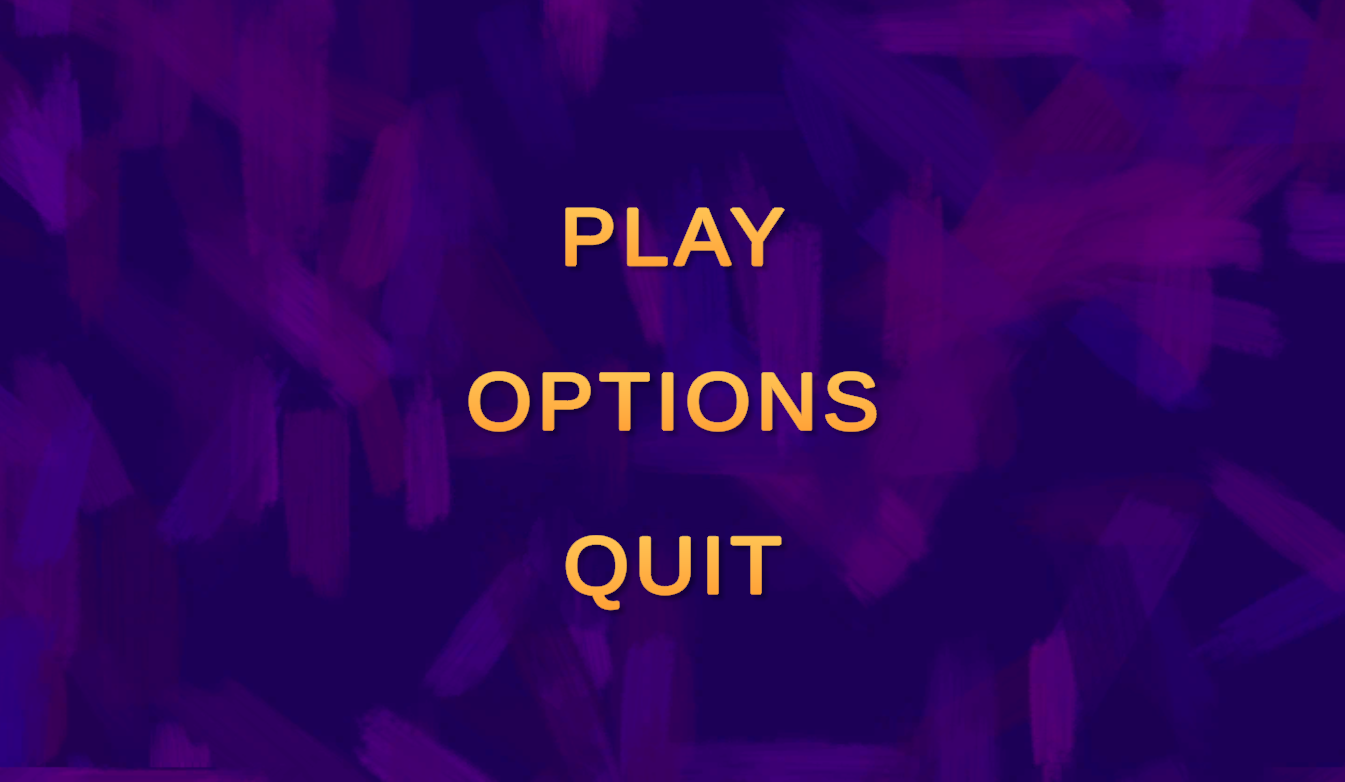
\includegraphics[width=\linewidth]{chapters/03/images/MainMenu.png}
        \caption{Das Hauptmenü des Prototyps.}
        \label{htl02a}
    \end{minipage}%
    \hspace{1cm}% Adjust the space here as needed
    \begin{minipage}{0.4\textwidth}
        \centering
        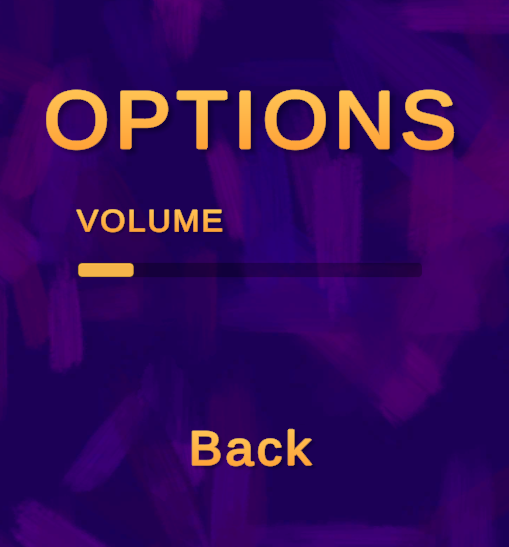
\includegraphics[width=\linewidth]{chapters/03/images/OptionsMainMenu.png}
        \caption{Das Optionsmenü des Prototyps.}
        \label{htl02b}
    \end{minipage}
\end{figure}

\section{Code behind des Menüs}

Der \bettergls{code-behind}{1} des Menüs ist sehr simpel gehalten und auch einfach zu verstehen.

% C#
\begin{lstlisting}[language=CSharp,caption={Main Menu Klasse.},label=code:mainmenu]
public class MainMenu : MonoBehaviour
{
    public void PlayGame()
    {
        var activeScene = SceneManager.GetActiveScene();
        SceneManager.LoadScene(activeScene.buildIndex + 1);
    }

    public void QuitGame()
    {
        Debug.Log("Quit");
        Application.Quit();
    }
}
\end{lstlisting}
Der SceneManager ist ein einfacher Weg mittels einer Art von \bettergls{statemachine}{2} eine Menüführung aufzubauen. In der nächsten Abbildung wird die Build-Reihenfolge der Scenes dargestellt.

\begin{center}
    \begin{figure}[h]
        \centering
        \includegraphics*[width=1\textwidth]{chapters/03/images/SceneManager.png}
        \caption{Der SceneManager in den Build Settings.}
        \label{htl04}
    \end{figure}
\end{center}

\noindent
Mittels der Code Zeile: 
% C#
\begin{lstlisting}[language=CSharp]
    SceneManager.LoadScene(activeScene.buildIndex + 1);
\end{lstlisting}
kann von der Menü Scene, die an der Stelle 0 ist zu der Projekt Scene, die an der Stelle 1 ist, gewechselt werden.

\pagebreak

\subsection{Die Funktion dem Button zuordnen}

In der nächsten Abbildung ist ein Ausschnitt der Properties des Play Buttons zu sehen. Bei der \verb+On Click ()+ Property wurde das \verb+MainMenu+ Skript hinzugefügt. Nachdem das Skript dort ausgewählt wurde, ist es möglich Methoden von diesem als Aktion für den Button auszuwählen. 

\begin{figure}[H]
    \centering
    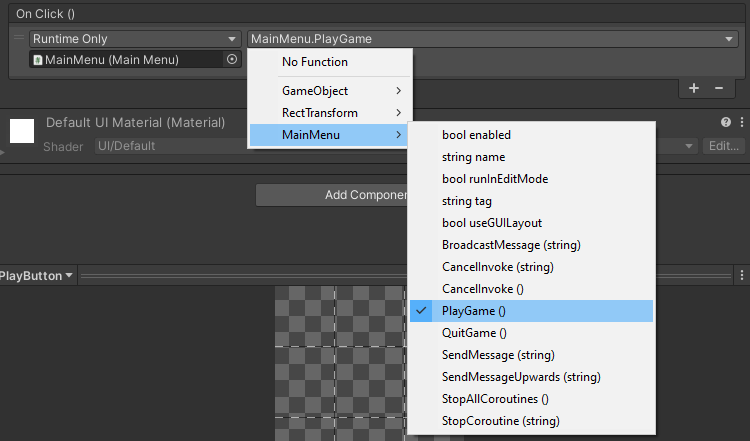
\includegraphics[width=0.6\textwidth]{chapters/03/images/PlayButton.png}
    \caption{Abbildung der Properties des Play Buttons.}
    \label{htl05}
\end{figure}

\section{Pausemenü und Game Over Screen}


Die Pause-Funktion ist ein wichtiger Teil eines Spiels, da sie den Spielern die Möglichkeit bietet, das Spiel zu pausieren, Einstellungen anzupassen oder sogar das Spiel zu verlassen, ohne den Fortschritt zu verlieren. Ebenso bedeutend ist der Game Over Screen, der dem Spieler nach einem Scheitern die Möglichkeit gibt, das Spiel neu zu starten oder komplett zu beenden.

\begin{figure}[H]
    \centering
    \begin{minipage}{0.4\textwidth}
        \centering
        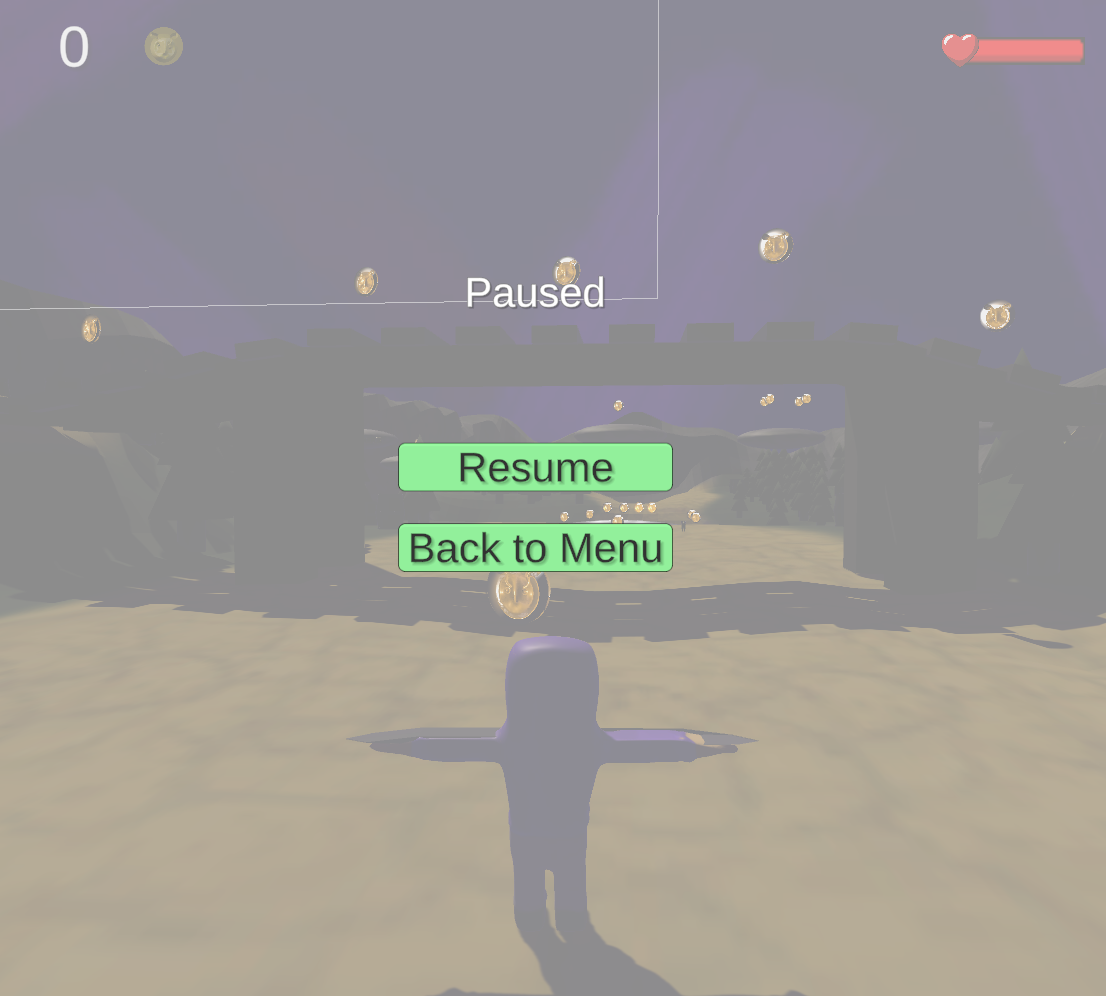
\includegraphics[width=\linewidth]{chapters/03/images/GamePaused.png}
        \caption{Das Game Paused UI des Prototypen.}
        \label{UI01}
    \end{minipage}
    \hspace{1cm}
    \begin{minipage}{0.4\textwidth}
        \centering
        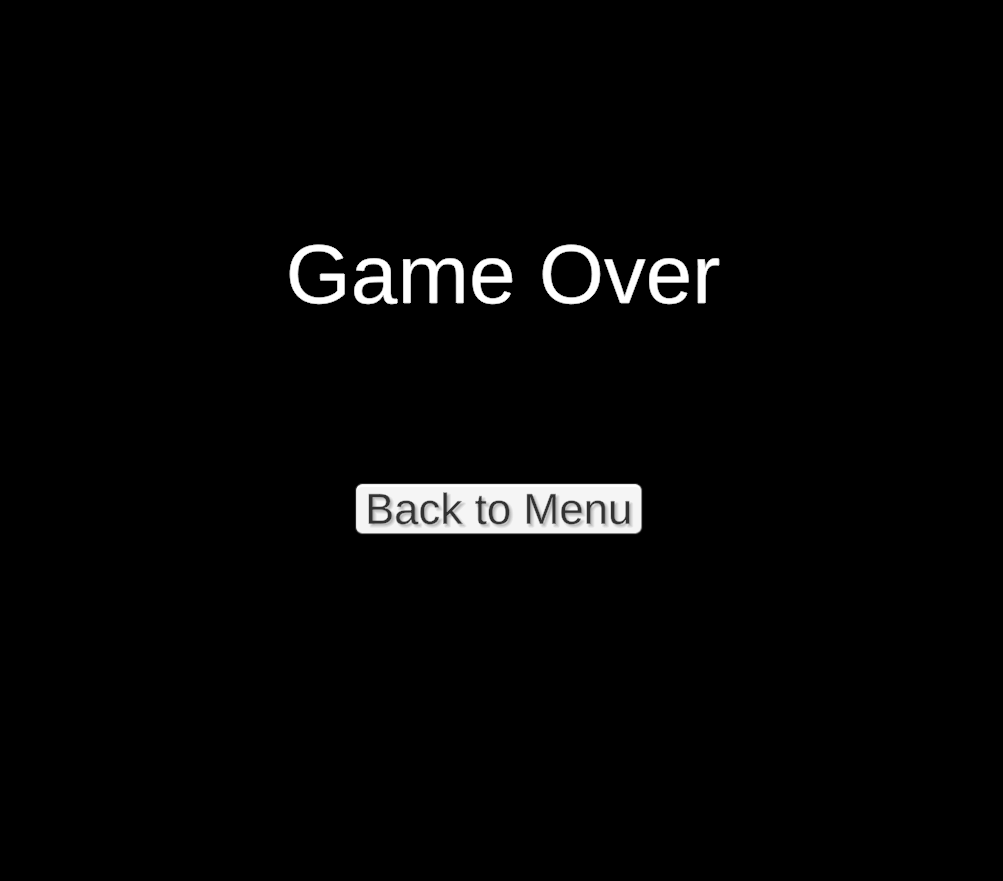
\includegraphics[width=\linewidth]{chapters/03/images/GameOver.png}
        \caption{Der Game Over Screen des Prototypen.}
        \label{UI02}
    \end{minipage}
\end{figure}



\section{Game UI und Spielmechanik-Anzeigen}

\begin{figure}[H]
    \centering
    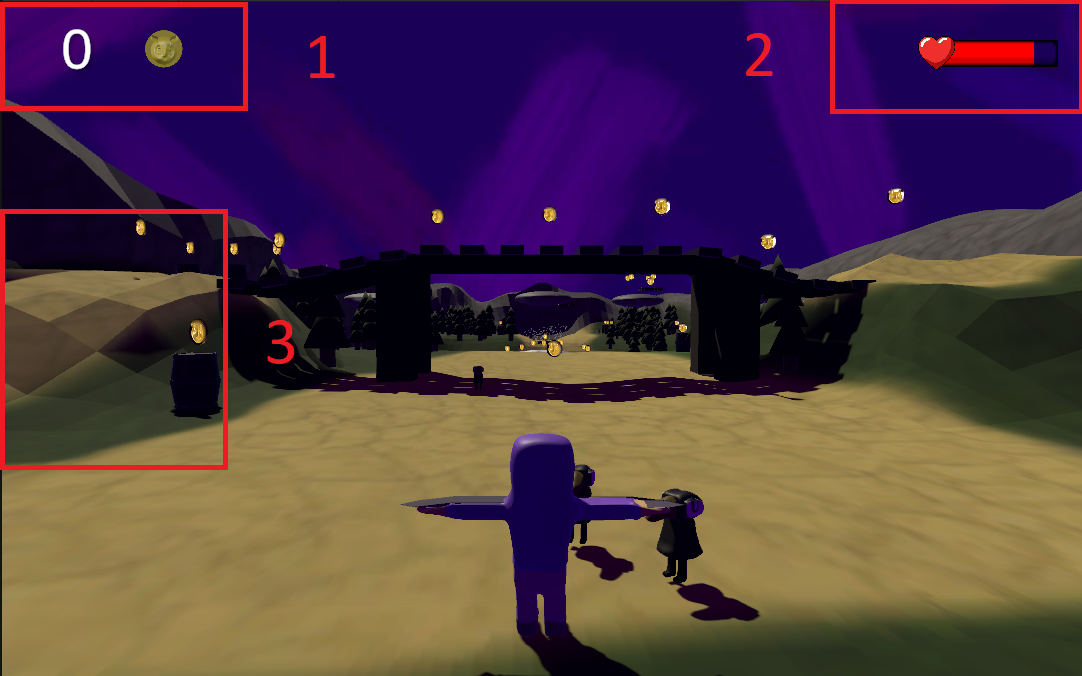
\includegraphics[width=0.8\textwidth]{chapters/03/images/GameUI.png}
    \caption{Das UI während des Spiels.}
    \label{htl03}
\end{figure}

\subsection{Eulenmünzen (1)}
Sammelobjekte, oder auch Collectibles gennant, gibt es in vielen Computerspielen. Jedoch bieten sie die unterschiedlichsten Funktionen. In PacMan ist das Sammeln von den Punkten teil des Spielziels. Verglichen zu Donkey Kong, wo das Sammeln von den Collectibles nicht verpflichtend ist. Aber es ist Teil von 101\% Vervollständigung des Spiels.
%https://donkeykong.fandom.com/wiki/Donkey_Kong_64#Gameplay

Als Sammelobjekt gibt es in dem Prototypen so gennante \glqq Eulenmünzen\grqq. Diese dienen ähnlich wie bei Donkey Kong als nicht verpflichtende Nebenaufgabe. Die Münzen schweben überall verstreut über die Welt des Prototypen. 

\subsection{Lebensanzeige (2)}

Eine Lebensanzeige in einem Computerspiel ist ein dezenter Hinweis darauf, dass der Spielcharakter sterblich ist. Schaden kann von Gegnern oder Fallen genommen werden.

In dem Prototypen wird die Lebensanzeige als roter Balken neben einem Herz dargestellt. Dieses Symbol befindet sich in der rechten oberen Ecke des Bildschirms. Lebensenergie wird abgezogen wenn die Spielfigur von einem Gegner getroffen wird oder in das \bettergls{void}{1} fällt.

\subsection{Steuerung (3)}
Die Idee war es die Steuerung auf dem User Interface darzustellen. Das ist ein einfacher Weg, das Spielkonzept dem Spieler näherzubringen. Ein gutes Beispiel dafür ist die Startwelt von Super Mario Odyssey. Dieses Spiel war auch eine große Inspiration für den Prototypen. 

%todo: level2 ui übergabe von wert... 67

\section{UI des zweiten Levels}

\begin{figure}[h]
    \centering
    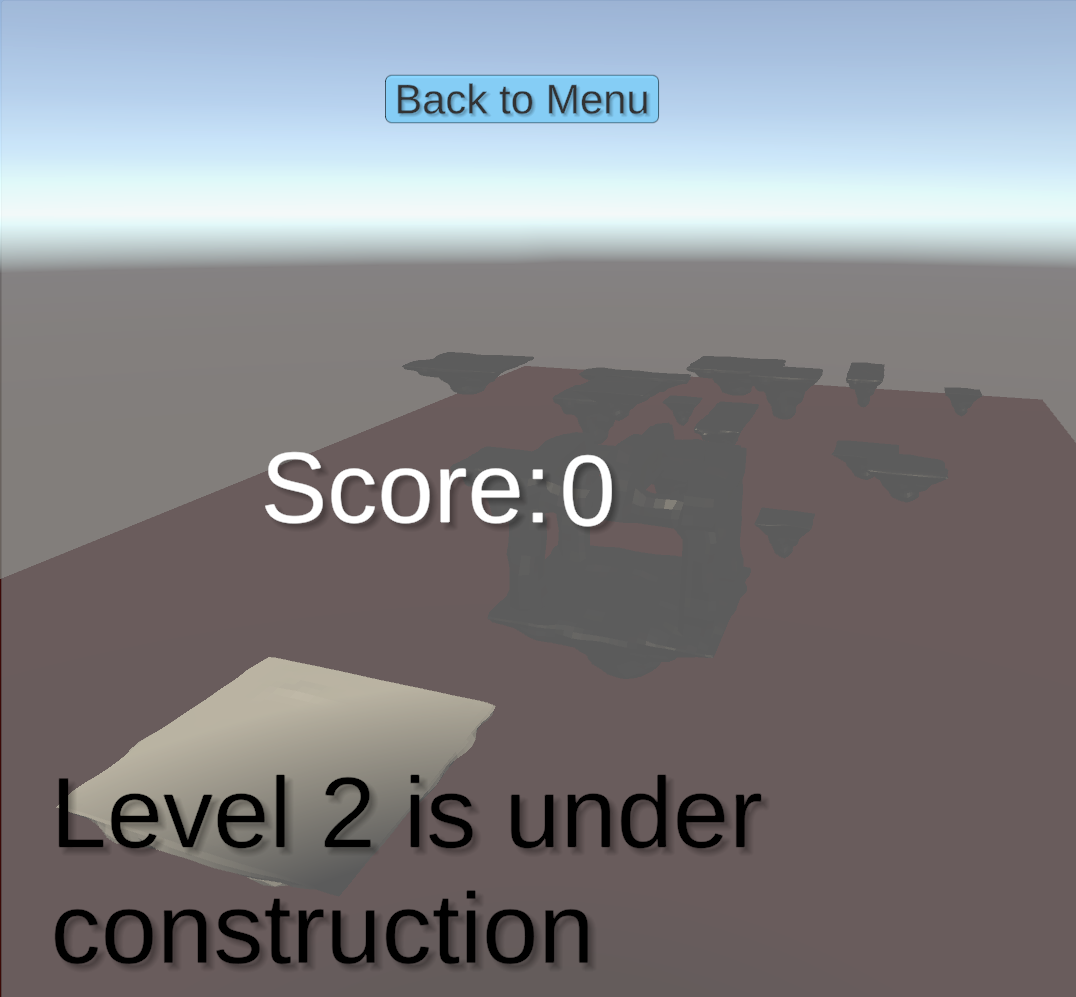
\includegraphics[width=0.6\textwidth]{chapters/04/images/V3/Level2Game.png}
    \caption{Der Endbildschirm des Prototypen.}
    \label{fig:UI20}
\end{figure}
\pagebreak
\chapter{Entwicklung des Prototyps}

In diesem Kapitel werden alle Schritte, die in die Kreation des Spiels hineingeflossen sind, beschrieben. Die Entwicklung des Prototypen fing mit der Idee des Themes an und durchlief mehere Phasen bis zur finalen Version des Spiels. Bei jeder dieser Phasen wurden viele Optimierungen gemacht und Fehler ausgebessert. 

\section{Einführung in die Ausgangsidee des Spiels}

Wegen des Vorwissens über Unity, welches in der 1 und 2.ten Klasse unterrichte wurde, war die Ausgangsidee für das Spiel eine einfache Wahl. Die fast einfachste und am weitesten verbreitete Kategorie von Spiel ist ein \bettergls{jumprun}{1}

\begin{quote}
  \emph{\glqq Ein Merkmal (von Jump'n'Run Spielen) sind die Plattformen. [...] Typisch beim Jump'n'Run ist das Verlieren\grqq}~\cite[Art of Gaming; 1:42-1:57]{ArtOfGaming}
\end{quote}

Ein Jump'n'Run würde einerseits kreative Freiheit über das Theme geben, aber auch die Möglichkeit bieten viele Aspekte der Spielentwicklung in dieser Diplomarbeit zu präsentieren.

\section{Beschreibung des gewählten Themes}

Da das Spiel nicht an der realen Welt entsprechen soll, kam die Überlegung eine Traumwelt zu bauen. In dieser gäbe es die Freiheit den Charakter, die Gegner und alle anderen Assets in verschiedenen Stilen zu designen. Damit wird auch für die Spieler des Prototypen klar, dass das gewählte Theme Fantasy ist. Zudem erleichtert diese Themenwahl dem Game-Designer die kreative Gestaltung.

\pagebreak

\section{Konzept und Anfangsschritte}
Das Konzept und die Anfangsschritte unterteilen sich in die folgenden Gebiete: 
\begin{itemize}
  \item Ideenfindung und Konzeptzeichnung für den ersten Prototypen (V1)
  \item Auswahl des Spielthemes und Design des Hauptcharakters
  \item Überlegung der grundlegenden Charaktersteuerung und Charakterfähigkeiten
\end{itemize}

Die ersten Schritte bei dem Entwickeln eines Videospiels beginnen immer mit einem Brain-Storming. Die ersten Ideen für diesen Prototypen waren das Theme, das Layout des ersten Levels und das ungefähre Design des Charakters.

\begin{figure}[h]
  \centering
  \begin{minipage}[b]{0.45\textwidth}
    \centering
    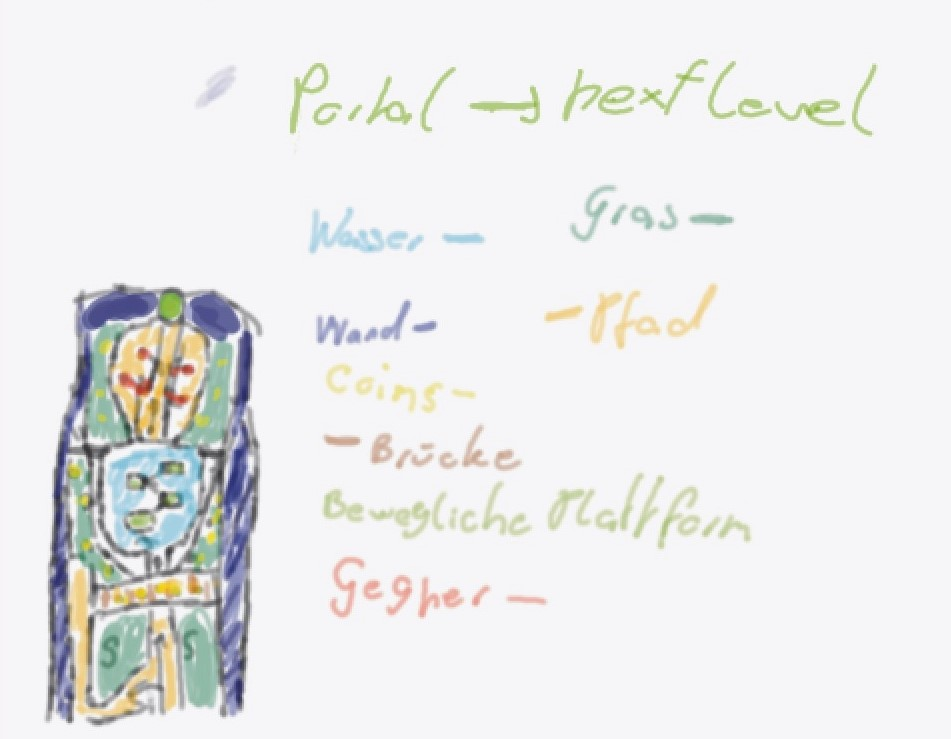
\includegraphics[width=\textwidth]{chapters/04/images/V1/drawing.jpg}
    \caption{Konzeptzeichnung und Ideenfindung.}
    \label{fig:PE01}
  \end{minipage}
  \hfill
  \begin{minipage}[b]{0.45\textwidth}
    \centering
    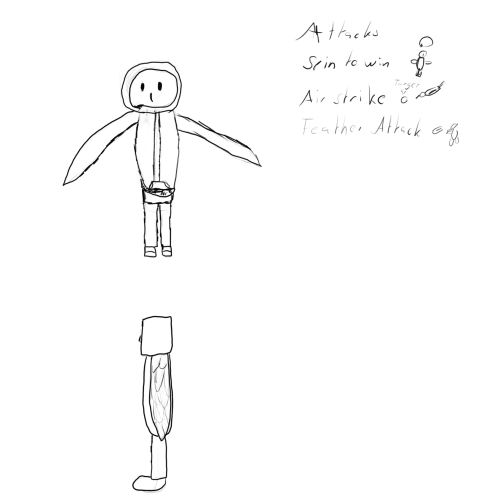
\includegraphics[width=\textwidth]{chapters/04/images/V1/CharScetch.png}
    \caption{Design des Hauptcharakters.}
    \label{fig:PE02}
  \end{minipage}
\end{figure}

In der Abbildung \ref{fig:PE01} sieht man die Konzeptzeichnung für das erste Level. In der Zeichnung ist eine von hohen Felsen abegrenzte Welt dargestellt. In der Mitte führt ein Pfad zu einem See. Über diesen schweben Plattformen. Über den Weg ist eine Holzbrücke auf der sich Münzen befinden. Die roten Punkte auf der anderen Seite des Wassers sind Gegner und am Ende des Pfades ist ein Portal, welches zum nächsten Level führt. In der rechten Abbildung \ref{fig:PE02} ist das erste Design des Hauptcharakters dargestellt. Die Überlegung war, eine kaputzentragende Eule mit einem Menschenkörper zu mischen. Die Zeichnung zeigt den Charakter von vorne und von der Seite. Der Text in der zweiten Abbildung ist eine Ideensammlung für die verschiedenen Attacken des Charakters. 
\pagebreak

\setauthorname{Lukas Schachinger \& Martin Usta}

\section{Version 1 des Prototypen}
In der Version 1 des Prototyps lag die Hauptkonztration in der schnellen Entwicklung eines Grundgerüsts des eigentlichen Prototypen. Dieser kann dann in den nächsten Versionen des Prototypen erweitert und verbessert werden. Ähnlich wie bei der agilen Projektentwicklung wurde die Entwicklung des Prototypen in verschiedene \glqq Sprints\grqq\space unterteilt. \\

Die zwei Hauptziele der Version 1 des Prototyen waren: 
\begin{itemize}
  \item Gestaltung des ersten Spiellevels im Rahmen des ersten Prototyps
  \item Programmierung von beweglichen Plattformen und Test von der Charaktersteuerung
\end{itemize}

\subsection{Prototyp V1 - Erstes Level:}

\begin{figure}[h]
  \centering
  \includegraphics*[width=0.6\textwidth]{chapters/04/images/V1/V1.png}
  \caption{Die erste Version des ersten Levels entwickelt in Unity.}
  \label{fig:PE03}
\end{figure}

Das erste Level des Prototypen wurde mit dem Unity Terrain Tool entworfen. Mit diesem Tool können Erhöhungen aus einer Platte erstellt werden. Genauso können Objekte wie Gräser und Bäume dynamisch auf den Grund des Levels plaziert und eingefärbt werden. \\\\
Dieses Tool ist zwar sehr mächtig, jedoch hat es auch seine Schwächen. Nach dem das Grundgerüst fertig war mussten noch Assets wie Bäume, Münzen und Gegner erstellt werden. Diese wurden in Blender modelliert und nach Unity exportiert. Beim Importieren war es wichtig, zu beachten, dass Unity und Blender ein Unterschiedliches Koordinatensystem verwendet. 

\pagebreak

\setauthorname{Lukas Schachinger}

\subsection{Programmierung der beweglichen Plattformen:}

Für die Programmierung der beweglichen Plattformen wurde ein leeres Unity Projekt angelegt. Dies bietet die Möglichkeit, ohne Auswirkungen auf den Prototypen zu Testen. Ein weiterer Vorteil ist, dass bei fatalen Fehlern einfach komplett neu begonnen werden kann. 

\begin{figure}[h]
  \centering
  \includegraphics*[width=0.6\textwidth]{chapters/04/images/V1/MovingPlatformV1.png}
  \caption{Die Entwicklung der beweglichen Plattform in einem leeren Projekt.}
  \label{fig:PE04}
\end{figure}

In der obigen Abbildung ist die Erstellung der beweglichen Plattformen dargestellt. Das weiße Rechteck ist die eigentliche Plattform auf der, der Charakter stehen kann. Die grüne Box außerhalb ist ein Box-\bettergls{collider}{1}. Dieser wurde für dieses Bild, für bessere Erkennbarkeit, vergrößert. Die drei blauen Punkte neben und über der Plattform sind die Wegpunkte für die Route der Plattform. Diese werden in dem \verb+WayPointFollower+ Skript angesprochen. \\

Bei dem Testen mit einer Spielfigur ist ein Problem aufgetreten ist. Die Plattform ist unter dem Charakter weggeflogen. Dabei hilft aber das \verb+StickyPlatform+ Skript. In diesem wird mit einem genialen Trick dieses Problem gelöst.\\

Das \verb+WayPointFollower+ Skript und auch das \verb+StickyPlatform+ Skript werden in dem \verb+Skripte+ Kapitel genauer beschrieben. 

\pagebreak


\subsection{Herausforderungen und Fortschritt:}
%\begin{itemize}
 % \item Bewältigung technischer Herausforderungen während der V1-Entwicklung
  %\item Erkennung von Leistungsproblemen aufgrund von Polygonanzahlen
 % \item Vorbereitung für die Optimierung in Version 2 des Prototyps (V2)
%\end{itemize}

Bei der ersten Version des Prototypen gab es noch viele Probleme. In den nächsten Punkten werden diese genauer Beschrieben. Welche Auswirkungen jeder dieser Fehler auf das Spiel hat und wie dieser behoben wurde.

\subsubsection{Unity Terrain Tools}
Bei der ersten Version war noch der Plan das erste Level mit den Unity Terrain Tools zu machen. Jedoch hat es sich schnell herausgestellt, dass dieses Tool nicht der richtige Ansatz für den Prototyen ist. Es gab Probleme bei dem Erstellen von dem Terrain und den schon erstellten Assets. Eine einfache Lösung dafür war, das Tool nichtmehr zu verwenden. Demnach der Umstieg auf Blender. Alle weiteren Versionen des Prototypen wurden mit Blender gemacht.

\subsubsection{Polygonanzahlen}
Assets wie die Brücke oder der Hauptcharakter wurden schon vorher in Blender erstellt. Es gab Unklarheiten bei der Auswirkung von hohen Polygonanzahlen. Diese beiden Assets wurden sehr detailliert modelliert. Das hatte die Auswirkung, dass bei dem Spielen des Prototypen die Perfomance gelitten hat. Lösung des Problemes war die neue Erstellung dieser Assets mit ungefähr 10.000 Polygonen anstatt 3 Millionen.

\subsubsection{Movement Skript}
Das Movement Skript der ersten Version hat ebenfalls gröbere Fehler enthalten. Der größte Fehler war die Verwendung der Funktion für die Bewegung der Spielfigur. Das Problem war, dass wenn der Player sich diagonal bewegte, wurde Bewegungsgeschwindigkeit von den zwei Richtungen addiert. Die Lösung des Problemes war, die Bewegungsrichtung zuerst herauszufinden und dann erst die Bewegungsgeschwindigkeit zu multiplizieren.

\pagebreak

\section{Version 2 des Prototyps}

Bei der zweiten Version des Prototypen musste das erste Level, der Charakter und andere Assets neu modelliert werden. Als neue addition kam das UI und weitere Assets dazu. Eine weiter Änderung war die farbliche Anpassung der Objekte an das Theme. 

\begin{figure}[h]
  \centering
  \begin{minipage}[b]{0.45\textwidth}
    \centering
    \includegraphics*[width=0.6\textwidth]{chapters/04/images/V2/char.png}
    \caption{Der neue Charakter für die V2 des Prototypen.}
    \label{fig:PE05}
  \end{minipage}
  \hfill
  \begin{minipage}[b]{0.45\textwidth}
    \centering
    \includegraphics*[width=0.6\textwidth]{chapters/04/images/V2/r4.png}
    \caption{Das Eulenmünzen Asset.}
    \label{fig:PE06}
  \end{minipage}
  \vfil
  \begin{minipage}[b]{1\textwidth}
    \centering
    \includegraphics*[width=1\textwidth]{chapters/04/images/V2/V2.jpg}
    \caption{Die zweite Version des ersten Levels.}
    \label{fig:PE07}
  \end{minipage}
\end{figure}

In den drei Abbildungen oberhalb ist der neue Charakter, die Eulenmünze und die zweite Version des ersten Levels dargestellt. Die Münze ist eines von vielen neu erstellten Assets. Unter anderem wurden noch Fässer, bewegliche Plattformen, Bäume und Steine modelliert.
\pagebreak

\subsection{Herausforderungen und Fortschritt:}

Bei der Erstellung der zweiten Version des Prototypen sind fast keine Probleme aufgetaucht. Die Entscheidung einen dritten Protoypen zu machen kam daher, weil die Entwicklung des Prototypen zu einem Stillstand gekommen ist. Eine gute Idee war der Neustart des Prototypen und daher der Anfang von der finalen Version. Ein weiterer Grund für den Neuanfang war, dass die zweite Version vom ersten Level nicht den selbst gesetzten Anforderungen entsprochen hat.  

\pagebreak

\section{Finaler Prototyp}

In der finalen Version des Prototypen lag das Ziel in der fertigstellung der Diplomarbeit reifen Endversion. Es wurden das erste Level und der Hauptcharakter erneut in Blender erstellt. Noch dazu wurden alle Skripte und das User Interface überarbeitet. 

\subsection{Level 1}

\begin{figure}[h]
  \centering
  \includegraphics*[width=0.8\textwidth]{chapters/04/images/V3/Level1.png}
  \caption{Die finale Version des ersten Levels mit allen Assets.}
  \label{fig:PE08}
\end{figure}

Die finalen Schritte bei dem ersten Level waren die Positionierung aller Assets, Münzen und Gegner. Die Erweiterung des User Interfaces. Zusätzlich die Implementation des Portales am Ende des Weges und des verbesserten AIs der Gegner.

\subsubsection{Gegner}


\begin{minipage}[t]{0.5\textwidth}
Diese Konzeptzeichnung der Gegner diente als Vorlage für die Enemy Game-Objekte. 
Sie sollen eine telepathische Krähe darstellen. In dem Prototypen suchen sie den Spieler und fügen ihm Schaden zu wenn sie nah genug herankommen.

\end{minipage}
\hfill
\begin{minipage}[t]{0.5\textwidth}
  \begin{figure}[H]
    \centering
    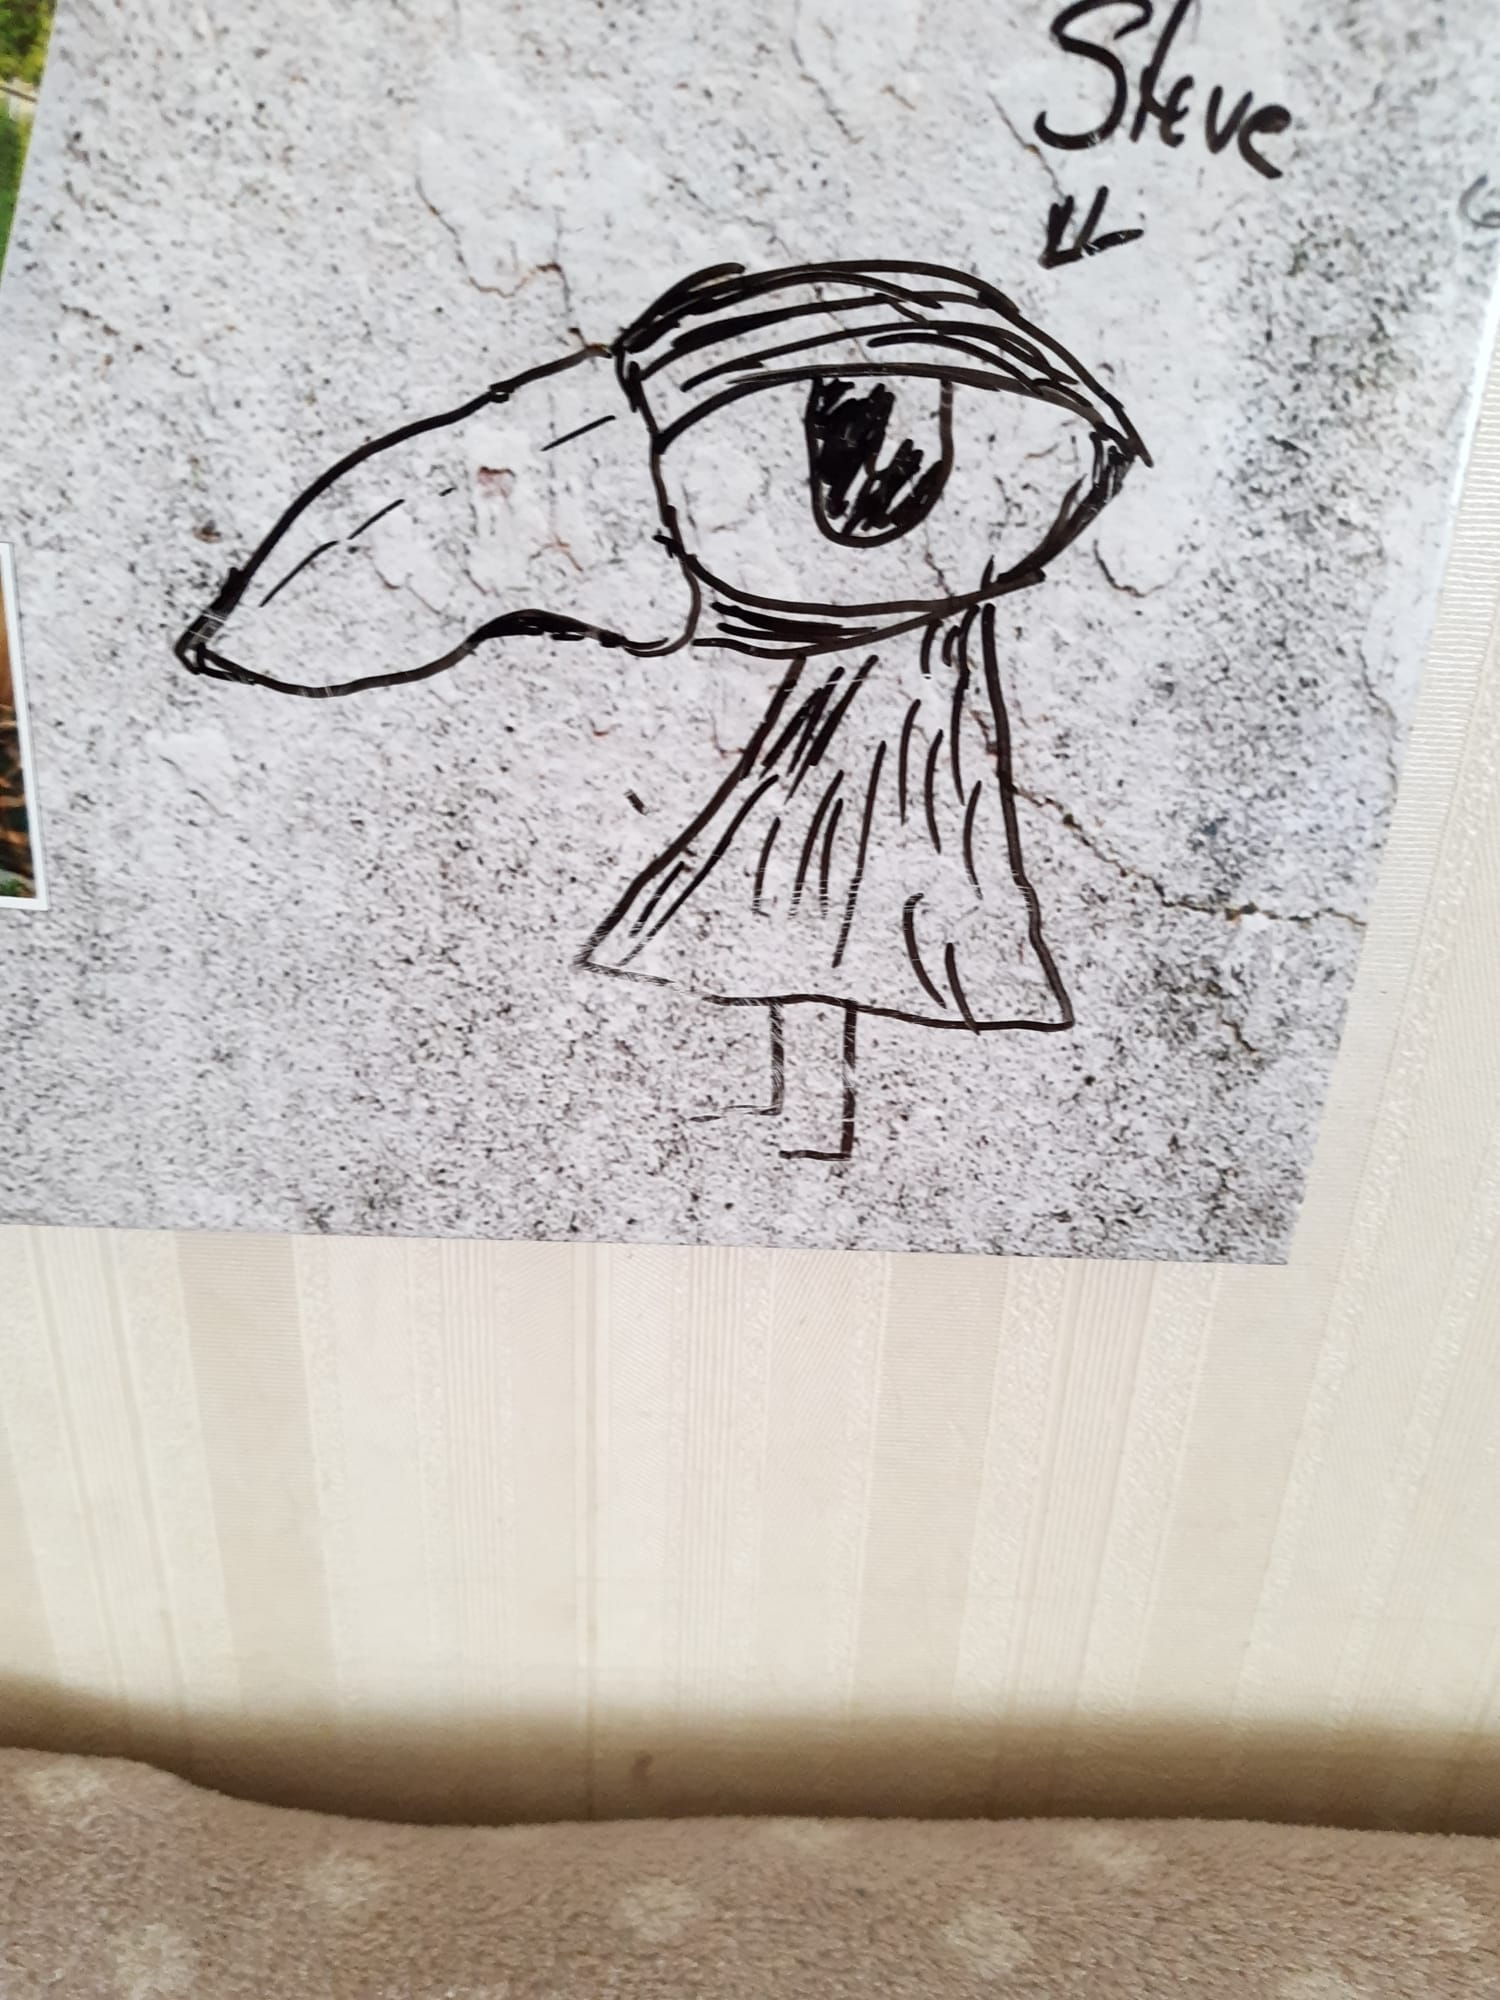
\includegraphics[width=0.8\textwidth]{chapters/04/images/V3/steve.jpg}
    \caption{Konzeptzeichnung des Gegners.}
  \end{figure}
\end{minipage}

\subsubsection{Das Portal}

\begin{minipage}[t]{0.4\textwidth}
  Das Portal war eine weitere Addition für den finalen Prototypen. Da das zweite Level schon begonnnen wurde, sollte es die Möglichkeit geben es vorzuführen. Das Portal besteht aus einer blauen, flachen Ebene mit wegschwebenden Partikeln. Das Skript ähnelt dem von der \verb+DeathZone+. Anstatt den Player zu dem Spawn zu teleportieren, wird die Scene gewechselt.

\end{minipage}
\hfill
\begin{minipage}[t]{0.6\textwidth}
  \begin{figure}[H]
    \centering
    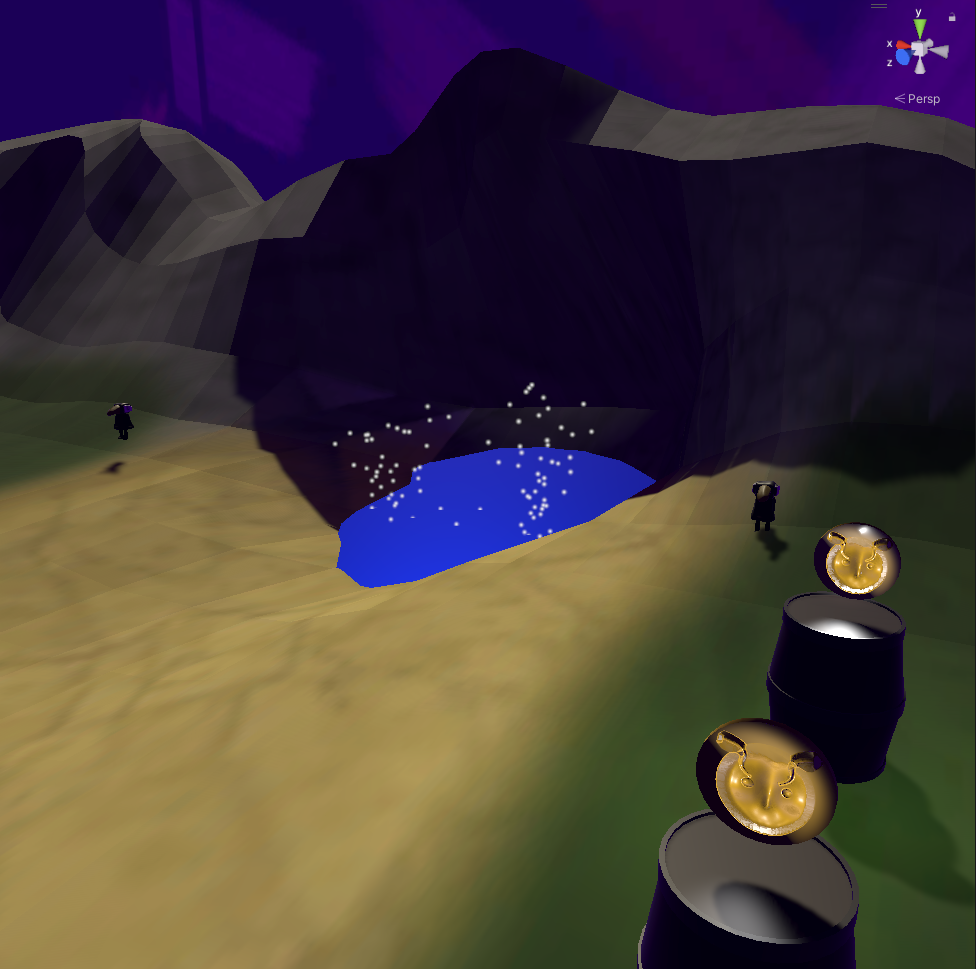
\includegraphics[width=0.8\textwidth]{chapters/04/images/V3/Portal.png}
    \caption{Das Portal zwischen dem ersten und zweiten Level.}
  \end{figure}
\end{minipage}


\pagebreak

\subsection{Level 2}
\begin{figure}[h]
  \centering
  \includegraphics*[width=0.6\textwidth]{chapters/04/images/V3/Level2.png}
  \caption{Das Grundgerüst des zweiten Levels.}
  \label{fig:PE09}
\end{figure}

Die Überlegung für das zweite Level war es, anschließend zu dem Portal im ersten Level, ein höhlen Level zu machen. In der Abbildung \ref{fig:PE09} sieht man den Ansatz des Leveldesigns. Der Boden soll Lava darstellen und das komplette Level soll sich innerhalb einer Höhle befinden. 
Das kann einfach erreicht werden indem ein das komplette Level in einem Quader platziert wird. Diesem müsste nur die Höhlenform ausgeschitten werden. Zum Zeitpunkt der Abgabe ist das Level noch unter \glqq Bauarbeiten\grqq \space und daher nur als Hintergrund des Endbildschirmes zu sehen. Siehe Abbildung \ref{fig:UI20}.

%In der finalen Version, wurde der Entschluss gefasst das die Map nochmal in Blender erstellt wird. Der Grund für diesen Schritt, dass in Blender die Tools ausgereifter für eine Level erstellung sind. Somit wirkt die Map schöner und perfomanter. Zudem gibt es schon Ansätze für das zweite Level. Aufgrund von zeitlichen Gründen haben wir es nicht geschafft das zweite Level fertig zustellen. In der letzten version wurde eine Animation für die Münzen erstellt. Die Münzen rotieren um ihre eigenen Achse herum sobald das Spiel startet. Das hat den zweck das Spiel lebhafter zu wirken. Zu dem wurde die Funtkion erstellt, das Münzen eingesammelt werden können. Die eingesammelten Münzen werden dann auf den oberen linken Eck des Bildschirms angezeigt. Weitere wurde das Letzte version des Spielbaren Charakters implmentiert. Aufgrund von zeitlichen gründen hat dieser keine Animation bekommen.  


\pagebreak



\pagebreak
\chapter{Scripte}

\section{Player Script}

\section{Enemy Script}

\section{Münzen Script}

\pagebreak
\setauthorname{Lukas Schachinger}

\chapter{Fazit}
Das letzte Kapitel dieser Diplomarbeit widmet sich der Frage: \glqq \textbf{Wie entwickelt man ein Computerspiel von Grund auf}\grqq. Während der Arbeit haben wir uns umfassend damit befasst, worauf es bei der Spielentwicklung ankommt. \\

Angefangen hat es mit der Überlegung des grundlegenden Konzeptes des Spiels. Zudem befassten wir uns mit dem Game Designs, der Storytelling-Elemente und der Spielmechaniken. Diese Teile sind das Grundgerüst jedes Spiels und legen den Grundstein für die gesamte Entwicklung.\\

Die technische Umsetzung ist der nächstwichtigste Punkt bei der Kreation eines Spieles. Zuerst muss man sich mit der Auswahl der richtigen Game Engine und Grafikdesigntools auseinandersetzen. Erst dann kann man sich mit der eigentlichen Entwicklung beschäftigen.\\

Wie in dem Kapitel \verb+Entwicklung des Prototyps+ beschrieben kann es passieren, dass mehere Versionen des Spieles erstellt werden muss. Dies ist ein großer Teil bei der Entwicklung eines Spieles. Diese Angehensweise ist hilfreich bei dem Testen oder der Verfeinerung der verschiedenen Aspekte des Spieles. In unserem Beispiel haben wir mehrere Versionen des ersten Levels erstellt um kleine Verbesserungen einzubauen oder bekannte Fehler auszubessern.\\

Zusammenfassend lässt sich sagen, dass die Spielentwicklung sowohl kreativ als auch technisch anspruchsvoll ist. Mit Hingabe und der Bereitschaft zum Lernen können Entwickler wie wir beeindruckende Spielerlebnisse erschaffen. Die sich stetig verändernde Branche eröffnet zudem Möglichkeiten, eigene Visionen zu verwirklichen und sich mit den neuesten Techniken zu beschäftigen.

%\addcontentsline{toc}{chapter}{Spielkonzept} 
%\addcontentsline{toc}{chapter}{Prototyp-Entwicklung}

%\addcontentsline{toc}{chapter}{Tests und Qualitätssicherung?}
%\addcontentsline{toc}{chapter}{Vermarktung und Veröffentlichung}
%\addcontentsline{toc}{chapter}{Zusammenfassung und Ausblick}
% todo: remove contents ^

\newpage
\appendix
\setauthorname{}

\newpage
\printnoidxglossaries

%\chapter*{Acknowledgements}
\addcontentsline{toc}{chapter}{Acknowledgements}

%\addcontentsline{toc}{chapter}{Listings}
%\lstlistoflistings

\addcontentsline{toc}{chapter}{List of Figures}
\listoffigures

\lstlistoflistings

\addcontentsline{toc}{chapter}{Bibliography}
\printbibliography

%
\chapter*{CV} \markboth{CV}{CV}
\addcontentsline{toc}{chapter}{CV}


\htlParagraph{Frieda Fröhlich}

\renewcommand{\arraystretch}{1.2}
\begin{tabularx}{1\textwidth}{@{} l X l @{}}

\emph{Geburtstag, Geburtsort:} & 01.01.1970, Braunau am Inn & 
\multirow{5}{2.5cm}{
    %\includegraphics[width=2.5cm]{./media/images/einstein.jpg}
} 
\\
\emph{Schulbildung:} & Volksschule \newline Hauptschule \newline HTL & \\
\emph{Praktika:} & Firmenname, Zeit, Tätigkeit & \\
\emph{Anschrift:} & Strasse Nummer\newline PLZ, Ort\newline Österreich & \\
\emph{E-Mail:} & frieda@froehlich.com & \\

\end{tabularx}
\\\\


\htlParagraph{Max Mustermann}

\begin{tabularx}{1\textwidth}{@{} l X l @{}}
\emph{Geburtstag, Geburtsort:} & 01.01.1970, Braunau am Inn & 
\multirow{5}{2.5cm}{
    %\includegraphics[width=2.5cm]{./media/images/einstein.jpg}
} 
\\
\emph{Schulbildung:} & Volksschule \newline Hauptschule \newline HTL & \\
\emph{Praktika:} & Firmenname, Zeit, Tätigkeit & \\
\emph{Anschrift:} & Strasse Nummer\newline PLZ, Ort\newline Österreich & \\
\emph{E-Mail:} & max@mustermann.com & \\

\end{tabularx}


\pagebreak
\htlParagraph{Max Mustermann}

\begin{tabularx}{1\textwidth}{@{} l X l @{}}
\emph{Geburtstag, Geburtsort:} & 01.01.1970, Braunau am Inn & 
\multirow{5}{2.5cm}{
    %\includegraphics[width=2.5cm]{./media/images/einstein.jpg}
} 
\\
\emph{Schulbildung:} & Volksschule \newline Hauptschule \newline HTL & \\
\emph{Praktika:} & Firmenname, Zeit, Tätigkeit & \\
\emph{Anschrift:} & Strasse Nummer\newline PLZ, Ort\newline Österreich & \\
\emph{E-Mail:} & max@mustermann.com & \\

\end{tabularx}
\chapter{Anhang}
\renewcommand{\arraystretch}{1}
\thispagestyle{empty}
\section{Begleitprotokolle}
\markboth{Begleitprotokolle}{Begleitprotokolle}
\newgeometry{bottom=10mm, left=20mm, right=30mm, top=30mm}

\pagebreak

\subsection{Begleitprotokoll Usta Martin}

\subsubsection{Stundenzahl nach Meilensteinen}

\begin{tabular}{|m{0.3\textwidth}|m{0.6\textwidth}|m{0.1\textwidth}|}
    \hline
    \cellcolor{gray!10} Datum & \cellcolor{gray!10} Meilenstein & \cellcolor{gray!10} Zeit in Stunden \\
    \hline
    9/2022 - 11/2022 & Analyse des Umfelds Projektplanung & 69 \\
    \hline
    11/2022 - 12/2022 & Erstellung des Grundgerüsts für den Prototyp & 69 \\
    \hline
    12/2022 - 02/2023 & Fertigstellung des UI & 69 \\
    \hline
    02/2023 - 05/2023 & Fertigstellung des Prototyps & 69 \\
    \hline
    05/2023 - 09/2023 & Diplomarbeit fertigstellen & 69 \\ 
    \hline
    \multicolumn{2}{|c|}{\cellcolor{gray!30}Gesamtdauer} & 69 \\
    \hline
\end{tabular}

\noindent

\vspace{40pt}

\subsubsection{Stundenerfassung}

\begin{tabular}{|m{0.3\textwidth}|m{0.6\textwidth}|m{0.1\textwidth}|}
    \hline
    \cellcolor{gray!10} Zeitraum & \cellcolor{gray!10} Tätigkeiten & \cellcolor{gray!10} Zeit in Stunden \\
    \hline
    9/2022 - 10/2022 & \hl{Beispiel: } Katalogisieren des Inventars & 69 \\
    \hline
    \multicolumn{2}{|c|}{\cellcolor{gray!30}Gesamtdauer} & 69 \\
    \hline
\end{tabular}

\pagebreak

\subsection{Begleitprotokoll Lukas Schachinger}

\subsubsection{Stundenzahl nach Meilensteinen}

\begin{tabular}{|m{0.3\textwidth}|m{0.6\textwidth}|m{0.1\textwidth}|}
    \hline
    \cellcolor{gray!10} Datum & \cellcolor{gray!10} Meilenstein & \cellcolor{gray!10} Zeit in Stunden \\
    \hline
    9/2022 - 11/2022 & Analyse des Umfelds/Projektplanung & 27 \\
    \hline
    11/2022 - 12/2022 & Erstellung des Grundgerüsts für den Prototyp & 37 \\
    \hline
    12/2022 - 02/2023 & Fertigstellung des UI & 17 \\
    \hline
    02/2023 - 05/2023 & Fertigstellung des Prototyps & 23 \\
    \hline
    05/2023 - 09/2023 & Diplomarbeit fertigstellen & 85 \\ 
    \hline
    \multicolumn{2}{|c|}{\cellcolor{gray!30}Gesamtdauer} & 189 \\
    \hline
\end{tabular}

\noindent

\vspace{40pt}

\subsubsection{Stundenerfassung}

\begin{tabular}{|m{0.206\textwidth}|m{0.7\textwidth}|m{0.094\textwidth}|}
    \hline
    \cellcolor{gray!10} Zeitraum & \cellcolor{gray!10} Tätigkeiten & \cellcolor{gray!10} Zeit in Stunden \\
    \hline
    9/2022 - 9/2022 & Ideensammlung für die Art des Spiels/das Theme/die Story & 8 \\
    \hline
    10/2022 - 11/2022 & Erstellung der Diplomarbeitsvorlage in LaTeX & 12 \\
    \hline
    11/2022 - 11/2022 & Erstellung des Pflichtenheftes & 7 \\
    \hline
    11/2022 - 12/2022 & Erstellung der Dokumentation & 7 \\
    \hline
    12/2022 - 12/2022 & Erstellung des Projektplanes & 5 \\
    \hline
    12/2022- 12/2022 & Recherche der Game Engines & 8 \\
    \hline
    10/2022 - 12/2022 & Entwicklung der ersten Version des Prototypen & 17 \\
    \hline
    12/2022 - 1/2023 & Recherche der wirtschaftlichen Begründung für die Entwicklung eines Spiels & 5 \\
    \hline
    1/2023 - 4/2023 & Entwicklung der zweiten Version des Prototypen & 24 \\
    \hline
    4/2023 - 9/2023 & Entwicklung der finalen Version des Prototypen & 37 \\
    \hline
    8/2023 - 9/2023 & Verfassen der Dokumentation & 32 \\
    \hline
    8/2023 - 9/2023 & Struktur der Dokumentation mit LaTeX anpassen & 8 \\
    \hline
    8/2023 - 9/2023 & Zusammenführung der beiden Dokumentationen des Diplomarbeit Teams & 10 \\
    \hline
    8/2023 - 9/2023 & Diplomarbeit überarbeiten und finalisieren & 9 \\
    \hline
    \multicolumn{2}{|c|}{\cellcolor{gray!30}Gesamtdauer} & 189 \\
    \hline
\end{tabular}


\pagebreak
\section{Betreuungsprotokolle} \markboth{Betreuungsprotokolle}{Betreuungsprotokolle}

% 111111111111111111111111111111111111111111111111111111111111111111111111111

\pagebreak

\noindent
\begin{tabular}{|m{0.2\textwidth}|m{0.6\textwidth}|m{0.2\textwidth}|}
\hline
\raisebox{-0.5\height}{
\includegraphics[width=1\linewidth]{media/images/htl-bildung-mit-zukunft.png}} 
&
\begin{center}
{\bfseries\sffamily\small HÖHERE TECHNISCHE BUNDES-LEHR- UND VERSUCHSANSTALT MÖDLING}\\[1ex]
{\small Höhere Lehranstalt für Elektronik und Technische Informatik\\
Kolleg für Informatik}
{\textcolor{gray}{bzw. Aufbaulehrgang für Informatik}}
\end{center} & 
\begin{center}
    {Reife- und Diplomprüfung}
\end{center} \\
\hline
\end{tabular}


\vspace*{20pt}
\subsection*{Betreuungsprotokoll zur Diplomarbeit \hfill lfd. Nr.: 1}
\vspace*{10pt}

\begin{tabular}{m{0.4\textwidth} m{0.4\textwidth}}
\textbf{Themenstellung:} & Unity Game Design und Development \\
\textbf{Kandidaten/Kandidatinnen:} & Schachinger Lukas, Usta Martin \\ \\
\textbf{Jahrgang:} & 2022/23 \\
\textbf{Betreuer/in:} & Hack Niklas \\
\textbf{Ort:} & Mödling \\
\textbf{Datum:} & 30.11.2022\\
\textbf{Zeit:} & 12:30 \\
\end{tabular}

\subsubsection*{Besprechungsinhalt:}
\begin{tabular}{|m{0.2\textwidth}|m{0.8\textwidth}|}
\hline
Name & Notiz \\
\hline
Usta, Schachinger & Anfang der Planung, Planung der Meilensteine, Einarbeitung des nächsten Meilensteins, Einrichten von DevOps Anfang der Umfeldanalyse \\
\hline
Usta & Aufgliederung der Meilensteine in Arbeitspackete,
Zuteilung der Arbeitspackete
Anfang der Umfeldanalyse von Designprogrammen,
2 von 3 wurden analysiert, Auswahlkriterien sind fertig\\
\hline
Schachinger & Aufgliederung der Meilensteine in Arbeitspackete, 
Zuteilung der Arbeitspakete
Anfang der Umfeldanalyse von Game Engines
1 von 3 wurden analysiert, Auswahlkriterien sind fertig\\
\hline
\end{tabular}

\subsubsection*{Aufgaben:}
\begin{tabular}{|m{0.2\textwidth}|m{0.6\textwidth}|m{0.2\textwidth}|}
\hline
Name & Notiz & zu erledigen bis \\
\hline
Usta & Fertigstellen der Umfeldanalysen 
Analyse von Designprogramm ZBrush & 12.12.2022 \\
\hline
Schachinger & Fertigstellen der Umfeldanalysen
Analyse von den Game Engines: Unreal, GoDot & 12.12.2022 \\
\hline
Usta & Grundgerüst Prototyp: 
Graphisches Leveldesign und erstellen der Low-Poly Assets
Implementierung der Charaktersteuerung & 18.12.2022 \\
\hline
Schachinger & Grundgerüst Prototyp: 
Implementierung der Bewegbaren Plattformen & 18.12.2022 \\
\hline
\end{tabular}

% 222222222222222222222222222222222222222222222222222222222222222222222222222

\pagebreak

\noindent
\begin{tabular}{|m{0.2\textwidth}|m{0.6\textwidth}|m{0.2\textwidth}|}
\hline
\raisebox{-0.5\height}{
\includegraphics[width=1\linewidth]{media/images/htl-bildung-mit-zukunft.png}} 
&
\begin{center}
{\bfseries\sffamily\small HÖHERE TECHNISCHE BUNDES-LEHR- UND VERSUCHSANSTALT MÖDLING}\\[1ex]
{\small Höhere Lehranstalt für Elektronik und Technische Informatik\\
Kolleg für Informatik}
{\textcolor{gray}{bzw. Aufbaulehrgang für Informatik}}
\end{center} & 
\begin{center}
    {Reife- und Diplomprüfung}
\end{center} \\
\hline
\end{tabular}


\vspace*{20pt}
\subsection*{Betreuungsprotokoll zur Diplomarbeit \hfill lfd. Nr.: 2}
\vspace*{10pt}

\begin{tabular}{m{0.4\textwidth} m{0.4\textwidth}}
\textbf{Themenstellung:} & Unity Game Design und Development \\
\textbf{Kandidaten/Kandidatinnen:} & Schachinger Lukas, Usta Martin \\ \\
\textbf{Jahrgang:} & 2022/23 \\
\textbf{Betreuer/in:} & Hack Niklas \\
\textbf{Ort:} & Mödling \\
\textbf{Datum:} & 19.12.2022 \\
\textbf{Zeit:} & 12:30 \\
\end{tabular}

\subsubsection*{Besprechungsinhalt:}
\begin{tabular}{|m{0.2\textwidth}|m{0.8\textwidth}|}
\hline
Name & Notiz \\
\hline
Usta & ZBrush noch nicht fertig analysiert \\
\hline
Usta & Leveldesign und Low-Poly fertig, Implementierung der Charaktersteuerung noch nicht fertig. \\
\hline
Schachinger & Umfeldanalyse für Unity und Unreal Engine fertig. Umfeldanalyse von GoDot noch nicht fertig. \\
\hline
Schachinger & Implementierung der bewegbaren Plattformen fertig. \\
\hline
\end{tabular}

\subsubsection*{Aufgaben:}
\begin{tabular}{|m{0.2\textwidth}|m{0.6\textwidth}|m{0.2\textwidth}|}
\hline
Name & Notiz & zu erledigen bis \\
\hline
Usta & ZBrush Umfeldanalyse fertigstellen & 28.02.2023 \\
\hline
Usta & Implementierung der Charaktersteuerung fertig & 28.02.2023 \\
\hline
Schachinger & GoDot Umfeldanalyse fertigstellen & 28.02.2023 \\
\hline
Schachinger, Usta & Planung des UI für eine optimale User Experience & 28.02.2023 \\
\hline
Schachinger & Aufbau und Erstellung einer Menu Führung & 28.02.2023 \\
\hline
Schachinger & Erstellung einer Statistikoberfläche & 28.02.2023 \\
\hline
\end{tabular}

% 333333333333333333333333333333333333333333333333333333333333333333333333333

\pagebreak

\noindent
\begin{tabular}{|m{0.2\textwidth}|m{0.6\textwidth}|m{0.2\textwidth}|}
\hline
\raisebox{-0.5\height}{
\includegraphics[width=1\linewidth]{media/images/htl-bildung-mit-zukunft.png}} 
&
\begin{center}
{\bfseries\sffamily\small HÖHERE TECHNISCHE BUNDES-LEHR- UND VERSUCHSANSTALT MÖDLING}\\[1ex]
{\small Höhere Lehranstalt für Elektronik und Technische Informatik\\
Kolleg für Informatik}
{\textcolor{gray}{bzw. Aufbaulehrgang für Informatik}}
\end{center} & 
\begin{center}
    {Reife- und Diplomprüfung}
\end{center} \\
\hline
\end{tabular}


\vspace*{20pt}
\subsection*{Betreuungsprotokoll zur Diplomarbeit \hfill lfd. Nr.: 3}
\vspace*{10pt}

\begin{tabular}{m{0.4\textwidth} m{0.4\textwidth}}
\textbf{Themenstellung:} & Unity Game Design und Development \\
\textbf{Kandidaten/Kandidatinnen:} & Schachinger Lukas, Usta Martin \\ \\
\textbf{Jahrgang:} & 2022/23 \\
\textbf{Betreuer/in:} & Hack Niklas \\
\textbf{Ort:} & Mödling \\
\textbf{Datum:} & 28.02.2023 \\
\textbf{Zeit:} & 12:30 \\
\end{tabular}

\subsubsection*{Besprechungsinhalt:}
\begin{tabular}{|m{0.2\textwidth}|m{0.8\textwidth}|}
\hline
Name & Notiz \\
\hline
Usta & ZBrush Umfeldanalyse muss noch überarbeitet werden. \\
\hline
Usta & Implementierung der Charaktersteuerung noch nicht fertiggestellt \\
\hline
Schachinger & GoDot Umfeldanalyse ist fertiggestellt. \\
\hline
Schachinger, Usta & Planung des UI für eine optimale User Experience. UI wurde neu erstellt, muss aber noch überarbeitet werden. \\
\hline
Schachinger & Aufbau und Erstellung einer Menu Führung noch nicht fertig, es fehlen Hauptmenü und Pausemenu.\\
\hline
Schachinger & Erstellung einer Statistikoberfläche fertiggestellt. \\
\hline
\end{tabular}

\subsubsection*{Aufgaben:}
\begin{tabular}{|m{0.2\textwidth}|m{0.6\textwidth}|m{0.2\textwidth}|}
\hline
Name & Notiz & zu erledigen bis \\
\hline
Usta & ZBrush Umfeldanalyse fertigstellen, anpassen auf das Layout & 20.03.2023 \\
\hline
Usta & Implementierung der Charaktersteuerung fertigstellen & 17.04.2023 \\
\hline
Schachinger & Planung des UI für eine optimale User Experience. UI überarbeiten und fertigstellen. & 20.03.2023 \\
\hline
Schachinger & Aufbau und Erstellung einer Menu Führung fertigstellen. & 17.04.2023 \\
\hline
Usta & Implementierung der High-Poly Assets & 31.05.2023 \\
\hline
Usta & Fertigstellung der Designaufgaben & 31.05.2023 \\
\hline
Schachinger & Fertigstellung der Programmieraufgaben & 31.05.2023 \\
\hline
\end{tabular}

% 444444444444444444444444444444444444444444444444444444444444444444444444444

\pagebreak

\noindent
\begin{tabular}{|m{0.2\textwidth}|m{0.6\textwidth}|m{0.2\textwidth}|}
\hline
\raisebox{-0.5\height}{
\includegraphics[width=1\linewidth]{media/images/htl-bildung-mit-zukunft.png}} 
&
\begin{center}
{\bfseries\sffamily\small HÖHERE TECHNISCHE BUNDES-LEHR- UND VERSUCHSANSTALT MÖDLING}\\[1ex]
{\small Höhere Lehranstalt für Elektronik und Technische Informatik\\
Kolleg für Informatik}
{\textcolor{gray}{bzw. Aufbaulehrgang für Informatik}}
\end{center} & 
\begin{center}
    {Reife- und Diplomprüfung}
\end{center} \\
\hline
\end{tabular}


\vspace*{20pt}
\subsection*{Betreuungsprotokoll zur Diplomarbeit \hfill lfd. Nr.: 4}
\vspace*{10pt}

\begin{tabular}{m{0.4\textwidth} m{0.4\textwidth}}
\textbf{Themenstellung:} & Unity Game Design und Development \\
\textbf{Kandidaten/Kandidatinnen:} & Schachinger Lukas, Usta Martin \\ \\
\textbf{Jahrgang:} & 2022/23 \\
\textbf{Betreuer/in:} & Hack Niklas \\
\textbf{Ort:} & Mödling \\
\textbf{Datum:} & 20.03.2023 \\
\textbf{Zeit:} & 10:30 \\
\end{tabular}

\subsubsection*{Besprechungsinhalt:}
\begin{tabular}{|m{0.2\textwidth}|m{0.8\textwidth}|}
\hline
Name & Notiz \\
\hline
Usta & ZBrush Umfeldanalyse fertiggestellt und auf ein einheitliches Layout angepasst. \\
\hline
Schachinger & UI noch nicht fertiggestellt Überarbeitung des Overlays (Münzen und Herzen) \\
\hline
\end{tabular}

\subsubsection*{Aufgaben:}
\begin{tabular}{|m{0.2\textwidth}|m{0.6\textwidth}|m{0.2\textwidth}|}
\hline
Name & Notiz & zu erledigen bis \\
\hline
Usta & Implementierung der Charaktersteuerung fertigstellen & 17.04.2023 \\
\hline
Schachinger & Überarbeitung des Overlays (Münzen und Herzen) & 17.04.2023 \\
\hline
Schachinger & Aufbau und Erstellung einer Menu Führung fertigstellen. & 17.04.2023 \\
\hline
Usta & Implementierung der High-Poly Assets & 31.05.2023 \\
\hline
Usta & Fertigstellung der Designaufgaben & 31.05.2023 \\
\hline
Schachinger & Fertigstellung der Designaufgaben & 31.05.2023 \\
\hline
\end{tabular}

% 555555555555555555555555555555555555555555555555555555555555555555555555555

\pagebreak

\noindent
\begin{tabular}{|m{0.2\textwidth}|m{0.6\textwidth}|m{0.2\textwidth}|}
\hline
\raisebox{-0.5\height}{
\includegraphics[width=1\linewidth]{media/images/htl-bildung-mit-zukunft.png}} 
&
\begin{center}
{\bfseries\sffamily\small HÖHERE TECHNISCHE BUNDES-LEHR- UND VERSUCHSANSTALT MÖDLING}\\[1ex]
{\small Höhere Lehranstalt für Elektronik und Technische Informatik\\
Kolleg für Informatik}
{\textcolor{gray}{bzw. Aufbaulehrgang für Informatik}}
\end{center} & 
\begin{center}
    {Reife- und Diplomprüfung}
\end{center} \\
\hline
\end{tabular}


\vspace*{20pt}
\subsection*{Betreuungsprotokoll zur Diplomarbeit \hfill lfd. Nr.: 5}
\vspace*{10pt}

\begin{tabular}{m{0.4\textwidth} m{0.4\textwidth}}
\textbf{Themenstellung:} & Unity Game Design und Development \\
\textbf{Kandidaten/Kandidatinnen:} & Schachinger Lukas, Usta Martin \\ \\
\textbf{Jahrgang:} & 2022/23 \\
\textbf{Betreuer/in:} & Hack Niklas \\
\textbf{Ort:} & Mödling \\
\textbf{Datum:} & 18.04.2023 \\
\textbf{Zeit:} & 10:00 \\
\end{tabular}

\subsubsection*{Besprechungsinhalt:}
\begin{tabular}{|m{0.2\textwidth}|m{0.8\textwidth}|}
\hline
Name & Notiz \\
\hline
Usta & Implementierung der Charaktersteuerung noch nicht fertiggestellt. \\
\hline
Schachinger & Überarbeitung des Overlays (Münzen und Herzen) fertiggestellt. \\
\hline
Schachinger & Pause und Quit Menu fertig, Spiel Hauptmenu noch nicht erstellt. \\
\hline
\end{tabular}

\subsubsection*{Aufgaben:}
\begin{tabular}{|m{0.2\textwidth}|m{0.6\textwidth}|m{0.2\textwidth}|}
\hline
Name & Notiz & zu erledigen bis \\
\hline
Schachinger & Spiel Hauptmenu erstellen. & 31.05.2023 \\
\hline
Usta & Charaktersteuerung muss überarbeitet werden. (Fähigkeiten und Text weiter verfassen) & 31.05.2023 \\
\hline
Usta & Implementierung der High-Poly Assets & 31.05.2023 \\
\hline
Usta & Fertigstellung der Designaufgaben & 31.05.2023 \\
\hline
Schachinger & Fertigstellung der Programmieraufgaben & 31.05.2023 \\
\hline
\end{tabular}

% 666666666666666666666666666666666666666666666666666666666666666666666666666

\pagebreak

\noindent
\begin{tabular}{|m{0.2\textwidth}|m{0.6\textwidth}|m{0.2\textwidth}|}
\hline
\raisebox{-0.5\height}{
\includegraphics[width=1\linewidth]{media/images/htl-bildung-mit-zukunft.png}} 
&
\begin{center}
{\bfseries\sffamily\small HÖHERE TECHNISCHE BUNDES-LEHR- UND VERSUCHSANSTALT MÖDLING}\\[1ex]
{\small Höhere Lehranstalt für Elektronik und Technische Informatik\\
Kolleg für Informatik}
{\textcolor{gray}{bzw. Aufbaulehrgang für Informatik}}
\end{center} & 
\begin{center}
    {Reife- und Diplomprüfung}
\end{center} \\
\hline
\end{tabular}


\vspace*{20pt}
\subsection*{Betreuungsprotokoll zur Diplomarbeit \hfill lfd. Nr.: 6}
\vspace*{10pt}

\begin{tabular}{m{0.4\textwidth} m{0.4\textwidth}}
\textbf{Themenstellung:} & Unity Game Design und Development \\
\textbf{Kandidaten/Kandidatinnen:} & Schachinger Lukas, Usta Martin \\ \\
\textbf{Jahrgang:} & 2022/23 \\
\textbf{Betreuer/in:} & Hack Niklas \\
\textbf{Ort:} & Mödling \\
\textbf{Datum:} & 31.05.2023 \\
\textbf{Zeit:} & 12:00 \\
\end{tabular}

\subsubsection*{Besprechungsinhalt:}
\begin{tabular}{|m{0.2\textwidth}|m{0.8\textwidth}|}
\hline
Name & Notiz \\
\hline
Usta & Charaktersteuerung muss noch überarbeitet werden. \\
\hline
Schachinger & Hauptmenu erstellt und implementiert. Settings müssen noch überarbeitet werden. \\
\hline
Usta & High Poly Assets erstellt muss noch implementiert werden. \\
\hline
Usta & Dokumentation über die Spiel Optimierung muss ausgebessert werden. \\
\hline
Schachinger & Programmieraufgaben sind noch nicht fertiggestellt. \\
\hline
Usta & Designaufgaben sind noch nicht fertiggestellt. \\
\hline
\end{tabular}

\subsubsection*{Aufgaben:}
\begin{tabular}{|m{0.2\textwidth}|m{0.6\textwidth}|m{0.2\textwidth}|}
\hline
Name & Notiz & zu erledigen bis \\
\hline
Schachinger & Settings im Pause Menu und im Haupt Menu überarbeiten. & 20.06.2023 \\
\hline
Usta & Charaktersteuerung muss weiter überarbeiten.  & 20.06.2023 \\
\hline
Usta & Implementierung der High-Poly Assets & 20.06.2023 \\
\hline
Usta & Fertigstellung der Designaufgaben & 20.06.2023 \\
\hline
Schachinger & Fertigstellung der Programmieraufgaben & 20.06.2023 \\
\hline
\end{tabular}

% 777777777777777777777777777777777777777777777777777777777777777777777777777

\pagebreak

\noindent
\begin{tabular}{|m{0.2\textwidth}|m{0.6\textwidth}|m{0.2\textwidth}|}
\hline
\raisebox{-0.5\height}{
\includegraphics[width=1\linewidth]{media/images/htl-bildung-mit-zukunft.png}} 
&
\begin{center}
{\bfseries\sffamily\small HÖHERE TECHNISCHE BUNDES-LEHR- UND VERSUCHSANSTALT MÖDLING}\\[1ex]
{\small Höhere Lehranstalt für Elektronik und Technische Informatik\\
Kolleg für Informatik}
{\textcolor{gray}{bzw. Aufbaulehrgang für Informatik}}
\end{center} & 
\begin{center}
    {Reife- und Diplomprüfung}
\end{center} \\
\hline
\end{tabular}


\vspace*{20pt}
\subsection*{Betreuungsprotokoll zur Diplomarbeit \hfill lfd. Nr.: 7}
\vspace*{10pt}

\begin{tabular}{m{0.4\textwidth} m{0.4\textwidth}}
\textbf{Themenstellung:} & Unity Game Design und Development \\
\textbf{Kandidaten/Kandidatinnen:} & Schachinger Lukas, Usta Martin \\ \\
\textbf{Jahrgang:} & 2022/23 \\
\textbf{Betreuer/in:} & Hack Niklas \\
\textbf{Ort:} & Mödling \\
\textbf{Datum:} & 20.06.2023 \\
\textbf{Zeit:} & 13:00 \\
\end{tabular}

\subsubsection*{Besprechungsinhalt:}
\begin{tabular}{|m{0.2\textwidth}|m{0.8\textwidth}|}
\hline
Name & Notiz \\
\hline
Schachinger & Menüführung muss noch finalisiert werden. \\
\hline
Schachinger & Finalisierung der Programmieraufgaben. \\
\hline
Usta & Charaktersteuerung muss noch finalisiert werden. \\
\hline
Usta & High-Poly Assets müssen noch fertiggestellt werden. \\
\hline
Usta & Finalisierung der Designaufgaben. \\
\hline
\end{tabular}

\subsubsection*{Aufgaben:}
\begin{tabular}{|m{0.2\textwidth}|m{0.6\textwidth}|m{0.2\textwidth}|}
\hline
Name & Notiz & zu erledigen bis \\
\hline
Schachinger & Fertigstellung der Menüführung. & 01.09.2023 \\
\hline
Schachinger & Finalisierung der Programmieraufgaben. & 01.09.2023 \\
\hline
Usta & Finalisierung der Charaktersteuerung.  & 01.09.2023 \\
\hline
Usta & Fertigstellung der High-Poly Assets. & 01.09.2023 \\
\hline
Usta & Finalisierung der Designaufgaben. & 01.09.2023 \\
\hline
\end{tabular}

\end{document}